\section{Nanoribbons}
\label{sec:nanoribbon}

In this section, we apply our code to the case of the honeycomb lattice of graphene and of the triangular lattice with the hoppings considered in the 3-band minimal model of \acs{TMD}s with intra-orbital on-site interactions.
We take boundary conditions corresponding to nanoribbons.
These structures are much longer on one direction than on the other, i.e. $l \gg w$, resembling a ribbon, hence their name (see Fig.(\ref{fig:bcRibbon}))\footnote{In Fig.(\ref{fig:bcRibbon}), this condition is, of course, not obeyed solely for the sake of giving a good visual representation of the boundary conditions, and the numbering system).}.
Along the $x$-direction, a ribbon is normally very long, which justifies the fact that we take \acp{PBC}.
In contrast, in the narrow $y$-direction we take \acp{OBC}.
The presence of low energy electronic states on the edges of these ribbons might lead to nontrivial magnetic behavior in \ac{TMD} nanostructures (as indeed they do in graphene nanostructures \cite{yazyev_emergence_2010}) and it is this possibility was unexplored numerically before this work \cite{feldner_dynamical_2011, golor_quantum_2013}, as was mentioned in chapter \ref{cap:int}.

\subsection{Graphene}
\label{sec:graphene}

We use three coordinates to label each site on the honeycomb lattice, by taking advantage of its bipartite nature.
Regarding the honeycomb lattice as two interpenetrating triangular sublattices $\mathcal{A}$ and $\mathcal{B}$, we take the axes $x$ and $y$ to be along the primitive vectors of each triangular sublattice.
To number the sites on the ribbon, we introduce an additional coordinate labeling the sublattice: $z = 0$, if the site is in sublattice $\mathcal{A}$, and $z = 1$ if the site is in sublattice $\mathcal{B}$.
We then adopt the numbering convention for the sites $i = 0,1, ..., 2 N_x N_y - 1$ of the lattice $\mathcal{L}$:
$
i (x, y, z) = N_x N_y z + N_x y + x,
$
 where $x = 0, ..., N_x - 1$, $y = 0, ..., N_y - 1$, and $z = 0, 1$ define each element $\bm r = (x, y, z) \in \mathcal{L}$.

The geometry of the system appears through the hopping matrix $\bm K$ in our code.
This numbering system makes it straightforward to find the neighbors of each site.
Let us begin by considering a site that is not on a zigzag edge.
There are two possible cases. For example, for 
$
z_i = 0, y_i \neq N_y - 1, x_i \neq 0 ,
$
 we have that the nearest neighbors of $i$ are $ j (i) = \{ j ( \bm r) \}$, with $\bm r$ in
\begin{equation*}
\bigg\{ \bm r_j \in \mathcal{L} \bigg| z_j = 1 \,\land\, \bigg[ \bigg( y_j = y_i  \,\land\, ( x_j = x_i \,\lor\, x_j = x_i - 1) \bigg) \,\lor\, \bigg( y_j = y_i + 1  \,\land\, x_j = x_i - 1  \bigg)  \bigg] \bigg\}
\end{equation*}

As opposed to the sites of a honeycomb lattice with \acp{PBC}, which have 3 neighbors, the sites of the zigzag edges have only 2 neighbors.
We summarize all possible cases in the following table.

\begin{table}[H]
\centering
	\caption{Nearest neighbors on the graphene nanoribbon.
	The neighbors in gray are only for sites that are not on the edges.
	$\%$ refers to the remainder of integer division.}
	\begin{tabular}{|c|c|c|c|} \hline
	\multicolumn{4}{|c|}{\textbf{\acp{OBC} \color{silver}{(\acp{PBC})} }}							\\ \hline
		Case 				& $z_j$	& $y_j$	& $x_j$ 	\\ \hline
		\multicolumn{1}{|c|}{\multirow{3}{*}{$z_i = 0$}}	 &	\multicolumn{1}{c|}{\multirow{3}{*}{1}} & \multicolumn{1}{c|}{\multirow{2}{*}{$y_i$}} & $x_i$   \\ \cline{4-4}
	   	\multicolumn{1}{|c|}{}	& \multicolumn{1}{c|}{\multirow{3}{*}{}} & \multicolumn{1}{c|}{\multirow{2}{*}{}}& \multicolumn{1}{c|}{\multirow{2}{*}{$N_x - 1 - (N_x - x_i) \% N_x$}} \\ \cline{3-3}
	   	\multicolumn{1}{|c|}{}	& \multicolumn{1}{c|}{} & \color{silver}{$y_i +1$} & \multicolumn{1}{c|}{\multirow{2}{*}{}} \\ \hline
		\multicolumn{1}{|c|}{\multirow{3}{*}{$z_i = 1$}}	 &	\multicolumn{1}{c|}{\multirow{3}{*}{0}} & \multicolumn{1}{c|}{\multirow{2}{*}{$y_i$}} & $x_i$   \\ \cline{4-4}
	   	\multicolumn{1}{|c|}{}	& \multicolumn{1}{c|}{\multirow{3}{*}{}} & \multicolumn{1}{c|}{\multirow{2}{*}{}}& \multicolumn{1}{c|}{\multirow{2}{*}{$(x_i + 1) \% N_x$}} \\ \cline{3-3}
	   	\multicolumn{1}{|c|}{}	& \multicolumn{1}{c|}{} & \color{silver}{$y_i -1$} & \multicolumn{1}{c|}{\multirow{2}{*}{}} \\ \hline
	\end{tabular}
	\label{tab:dummytable}
\end{table}

Recall the mean field result obtained for a graphene nanoribbon we presented in chapter \ref{cap:int}.
For each sublattice, ferromagnetic order is induced by the on-site interaction along each row of the ribbon, i.e. along the longitudinal direction $x$.
The average spin density has its maximum on the edge, decaying in the bulk.
It reaches another (smaller) maximum on the other side of the ribbon, i.e., in the row next to the other sublattice's edge (see Fig.(\ref{fig:nanoGraphVsTMD})).
This type of global antiferromagnetic ordering (considering the two sublattices) is confirmed by \ac{QMC} \cite{feldner_dynamical_2011, raczkowski_interplay_2017}.
Other recent auxiliary field \ac{QMC} studies point at the possibility of strain-tuning this type of edge-magnetism in zig-zag graphene nanoribbons \cite{yang_strain-tuning_2017}.
The authors start by introducing a reduction in the hopping along $x$ to model strain, i.e. changing the hopping between atoms connected by red bonds in Fig.(\ref{fig:bcRibbon}): $-t \mapsto -t + \Delta$.
Then, they identify phase transitions to edge-magnetized states for relatively small values of the hopping reduction ($\Delta = 0-0.5t$) and on-site interaction ($U = (1 - 4) t$).
To do so, they fit the susceptibility at the edge $\chi_e$ to the Curie-Weiss law:
\begin{equation}
\frac{1}{\chi_e} = \frac{T - T_c}{A} ,
\end{equation}
and identify the critical temperature.
By repeating this procedure for different simulations, one can find critical values of $U_c$ and $\Delta$ for the transition to occur, and find the critical temperatures of the transitions for different values of these parameters.

\begin{figure}[H]
\hspace{-0.8cm}
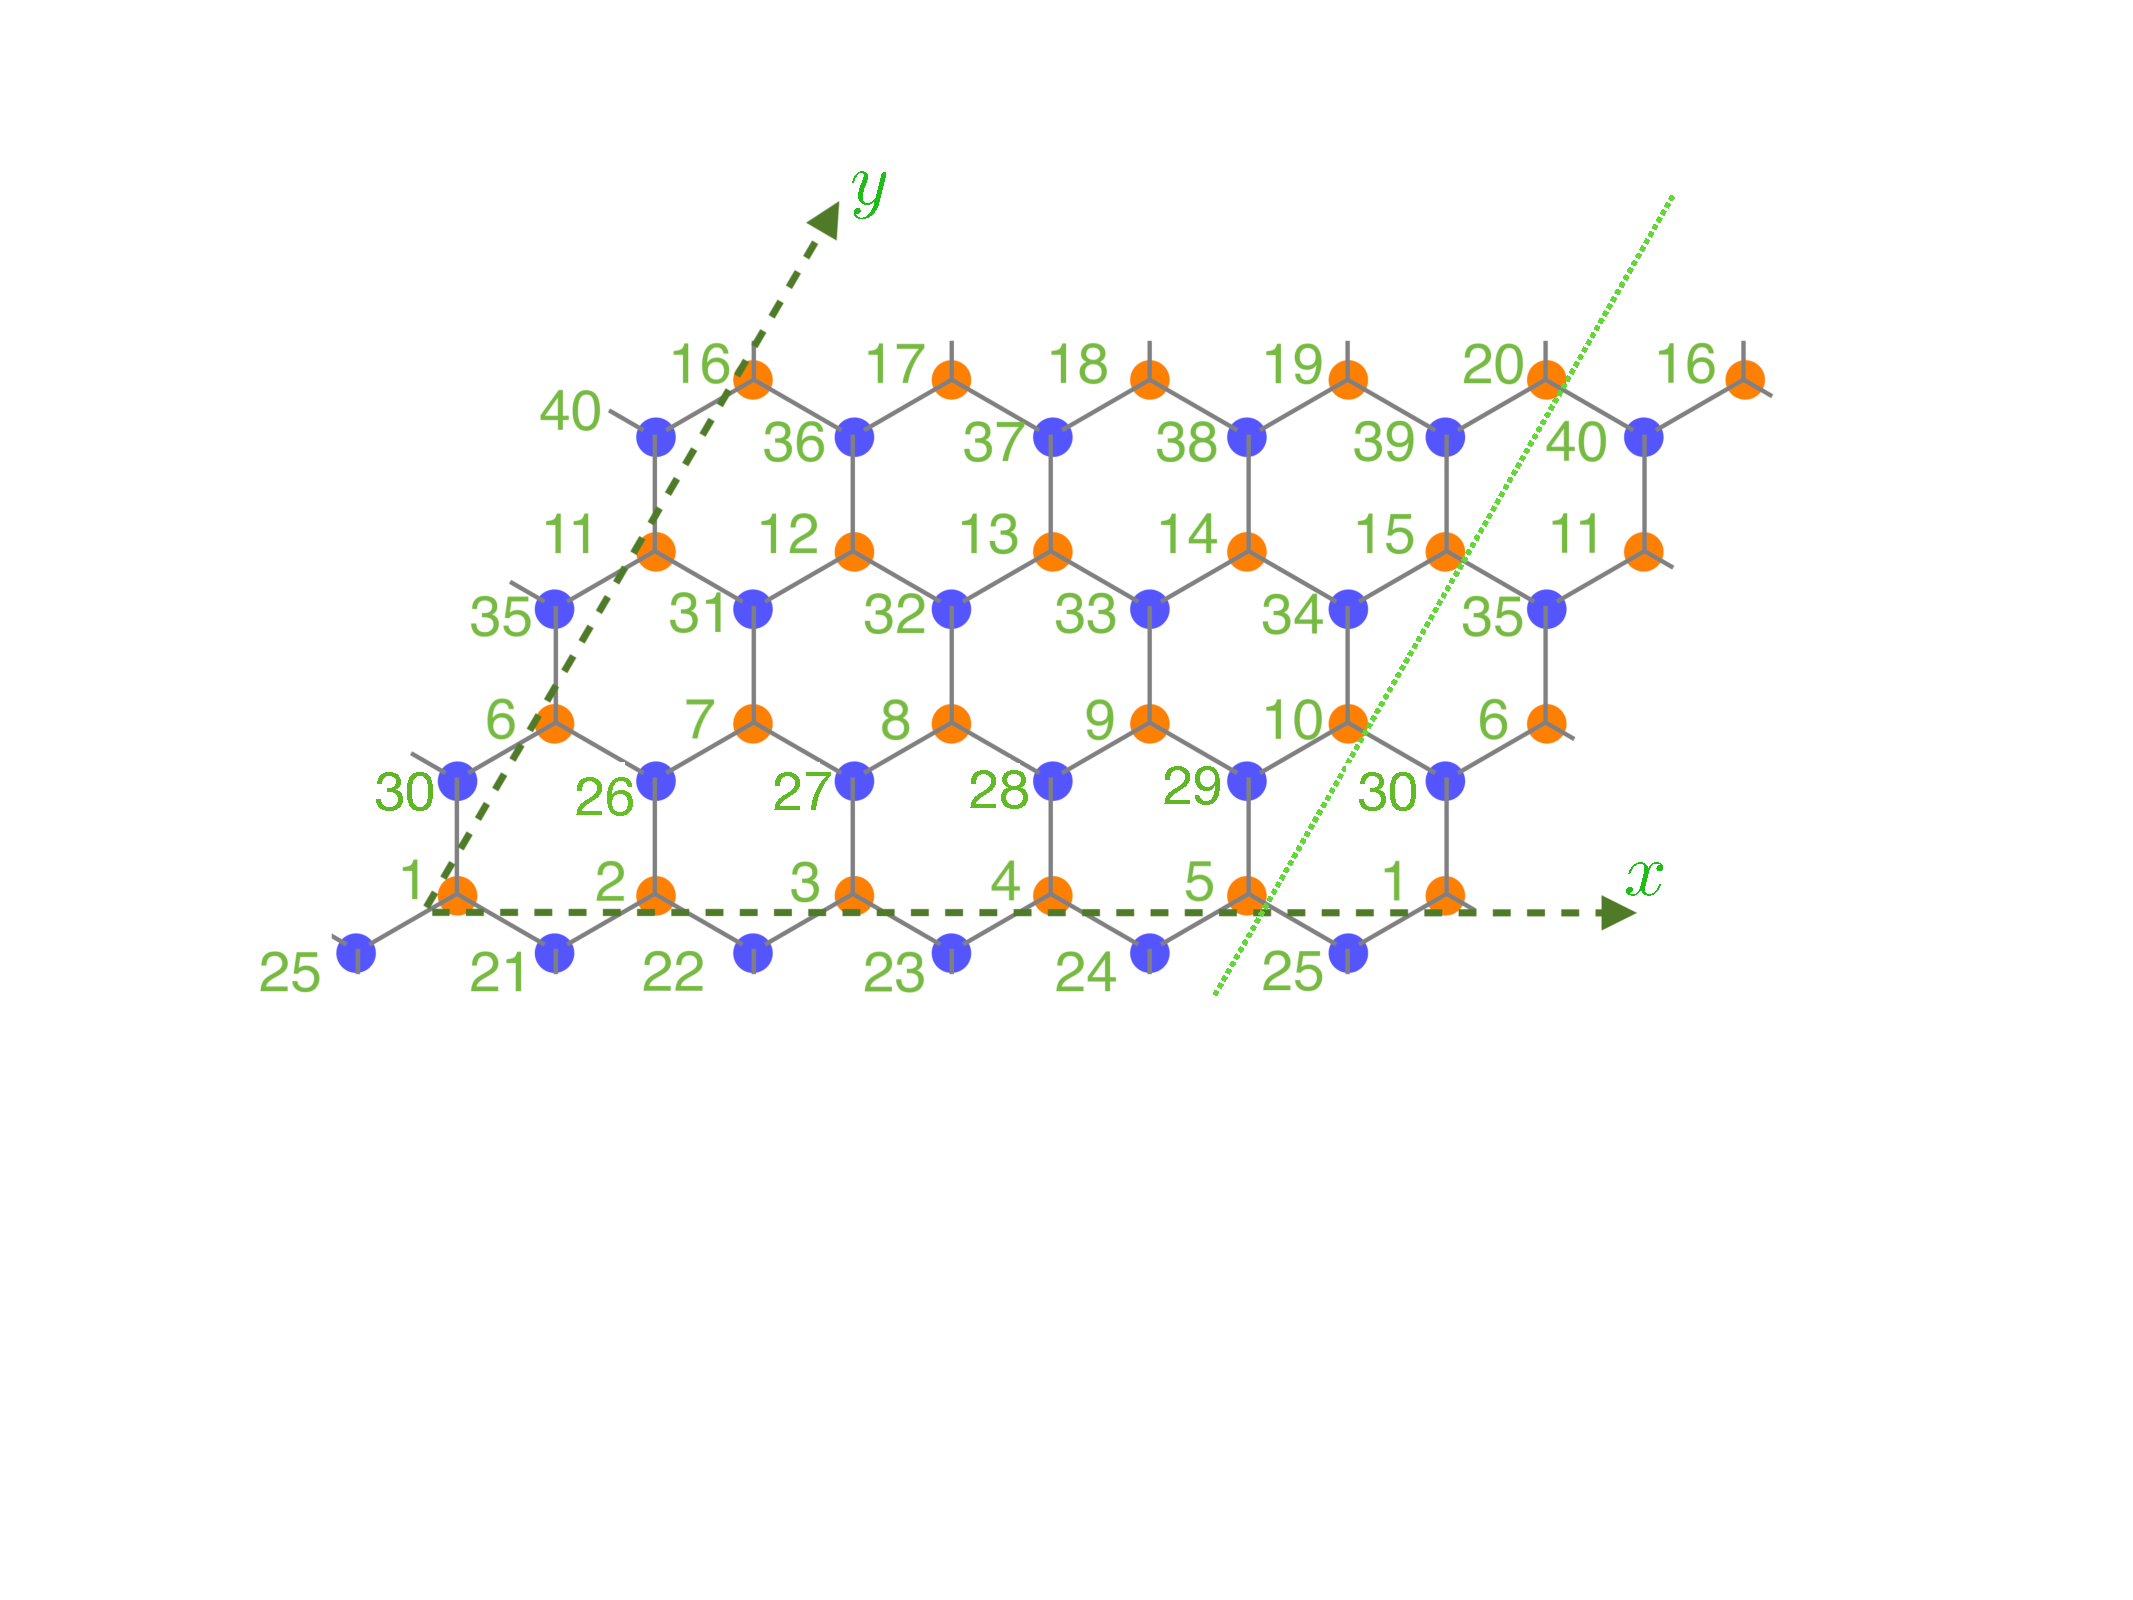
\includegraphics[trim={0 8cm 0 2.5cm},clip, scale = 0.27]{Applications/nanoribbon.pdf}
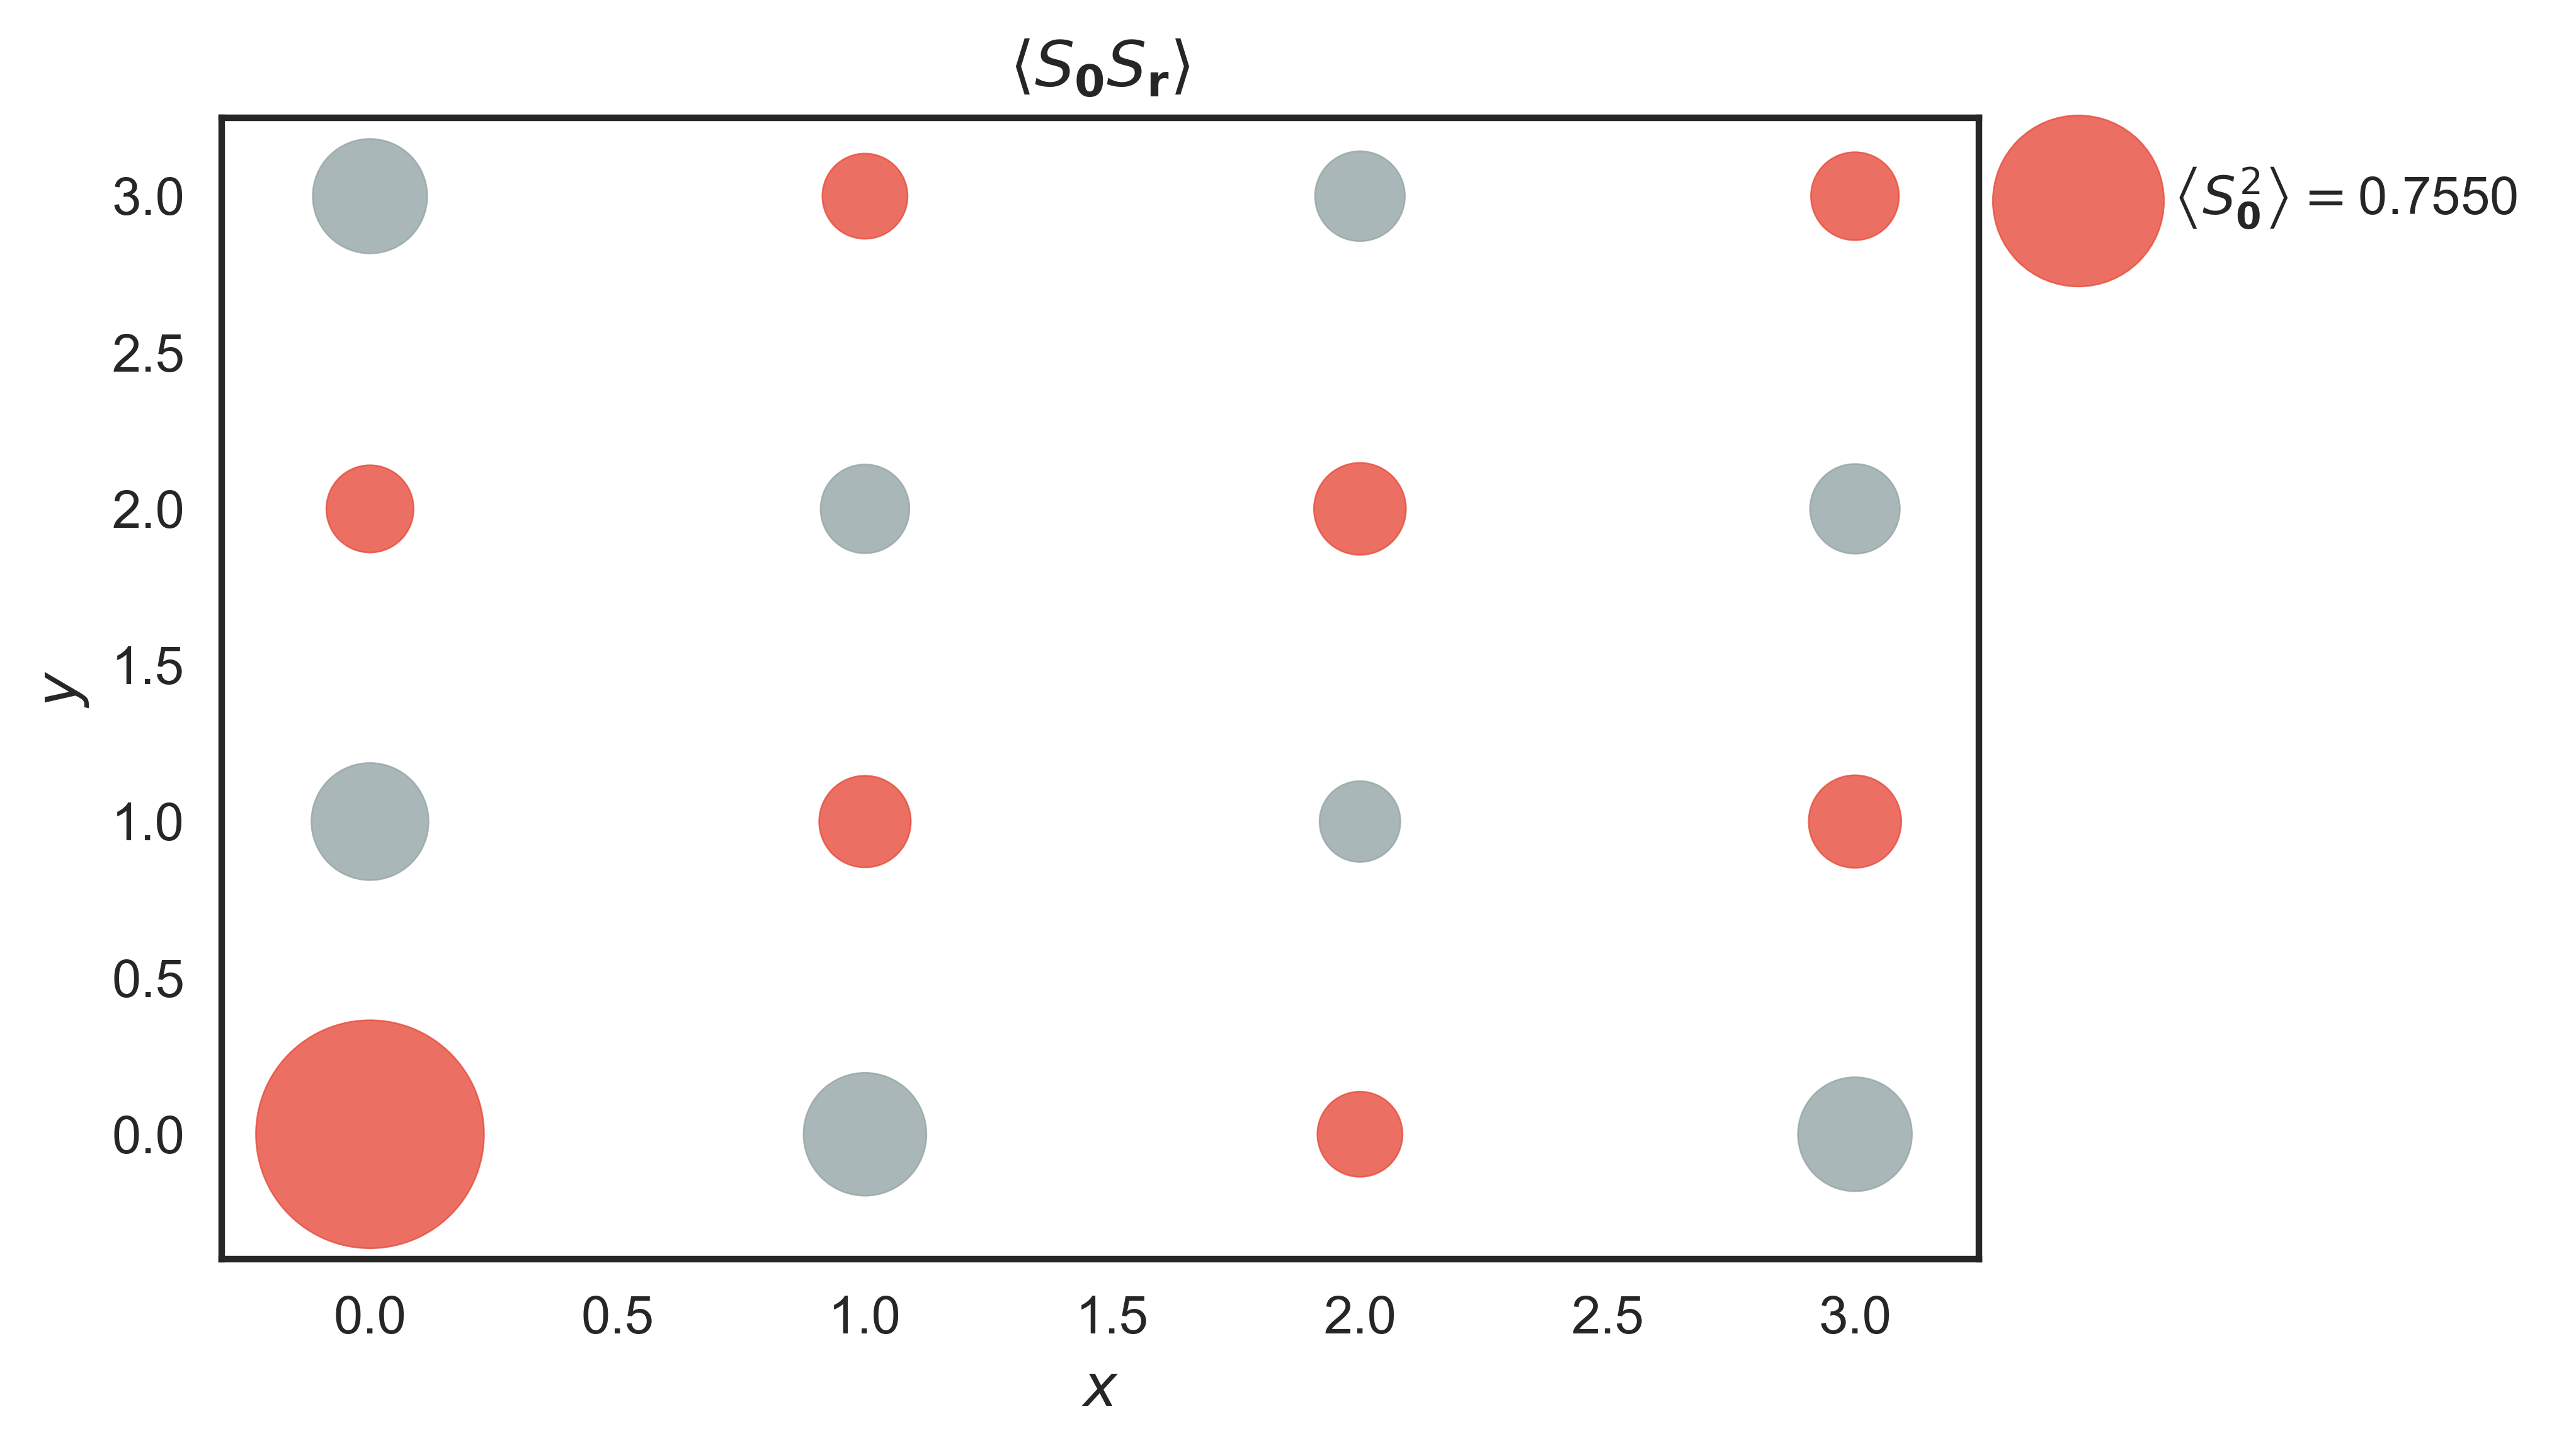
\includegraphics[scale = 0.49]{Applications/graphene-strain/CorrelationsDots.png}
	\caption[Boundary conditions on the nanoribbon. Spin-spin correlations of a strained zig-zag graphene nanoribbon.]{Left: Boundary conditions on the nanoribbon for $N_x = 5, \, N_y = 4$. The orange circles correspond to sublattice $\mathcal{A}$, and the blue circles correspond to sublattice $\mathcal{B}$.
	Spin-spin correlations of a strained zig-zag graphene nanoribbon, with reduced hopping along $x$: $t \mapsto t - \Delta$, for $\Delta = 0.3t$. The label $\bm 0$ refers to the lower left site.
}
	\label{fig:bcRibbon}
\end{figure}

Any kind of mean field treatment tends to overestimate long range order.
In this case, it predicts spin correlations to decay rapidly from the edge rows inward, and then to remain constant along the $x$ direction \cite{feldner_dynamical_2011}.
The \ac{QMC} result of Fig.(\ref{fig:bcRibbon}) shows us that it decays along the periodic $x$-direction, and then increases again, with the profile shown in Fig.(\ref{fig:longProf}).
This is a typical result for this type of nanostructure, and it generally indicates long range order.
For example, in \cite{feldner_dynamical_2011}, it is shown that by increasing the width of ribbon, the correlations decay less and less until they almost reach the type of behavior predicted by mean field.

A peak at $\bm q = \bm 0$ in the magnetic structure factor $S ( \bm q )$ suggests sublattice ferromagnetic ordering, and indeed, by studying the magnetic structure factor of each row separately, we see that it is enhanced at $\bm q = \bm 0$ on the edges compared to the bulk.
Moreover, we study the behavior of the function $M_{\text{row}} \equiv \frac{1}{N_x}\sqrt{ \sum_{(i, j) \in \text{row}} \left\langle S_i S_j \right\rangle}$, and we conclude that it is maximum in one of the edge rows, decreases as we penetrate the bulk, and then increases again, having a smaller local maximum on the other edge row.
This is an indication of edge-magnetism, qualitatively similar to what is obtained in mean field.
If we had more CPU time available, we could do larger scale simulations to see a more dramatic effect on \emph{both} edges relative to the bulk.

\begin{figure}[H]
\hspace{0.3cm}
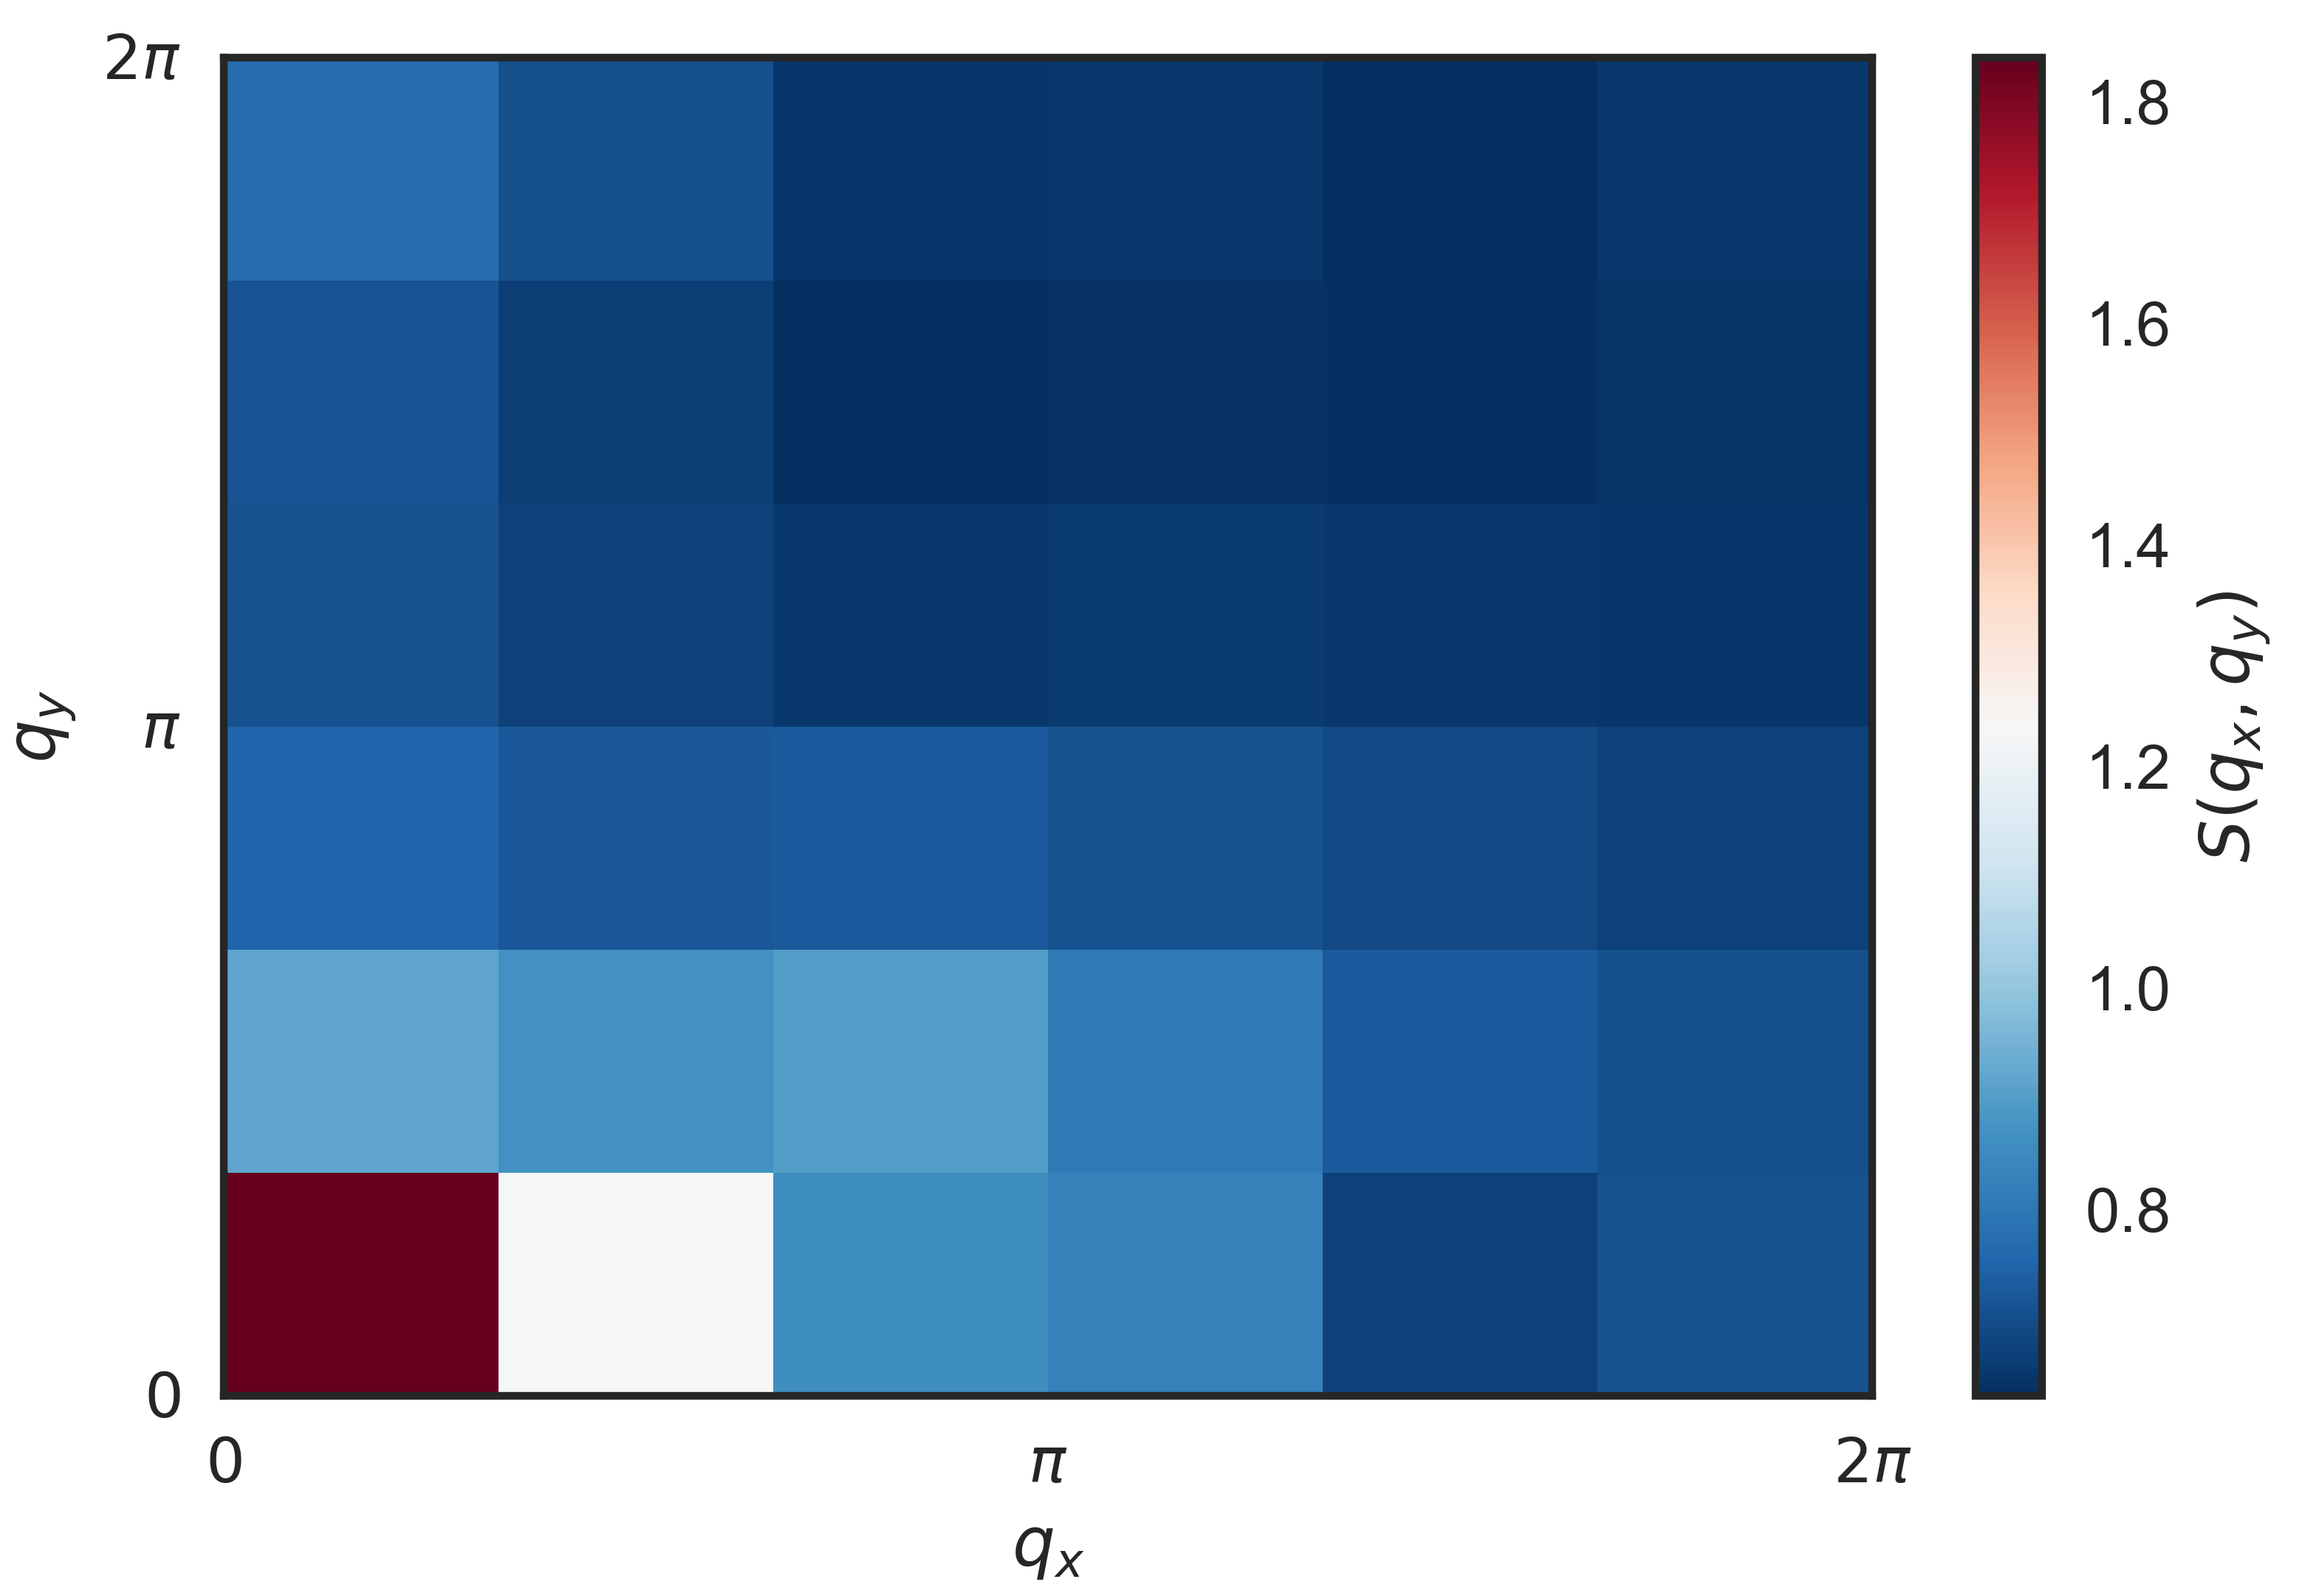
\includegraphics[scale = 0.55]{Applications/graphene-strain/S(q)pcolor.png}
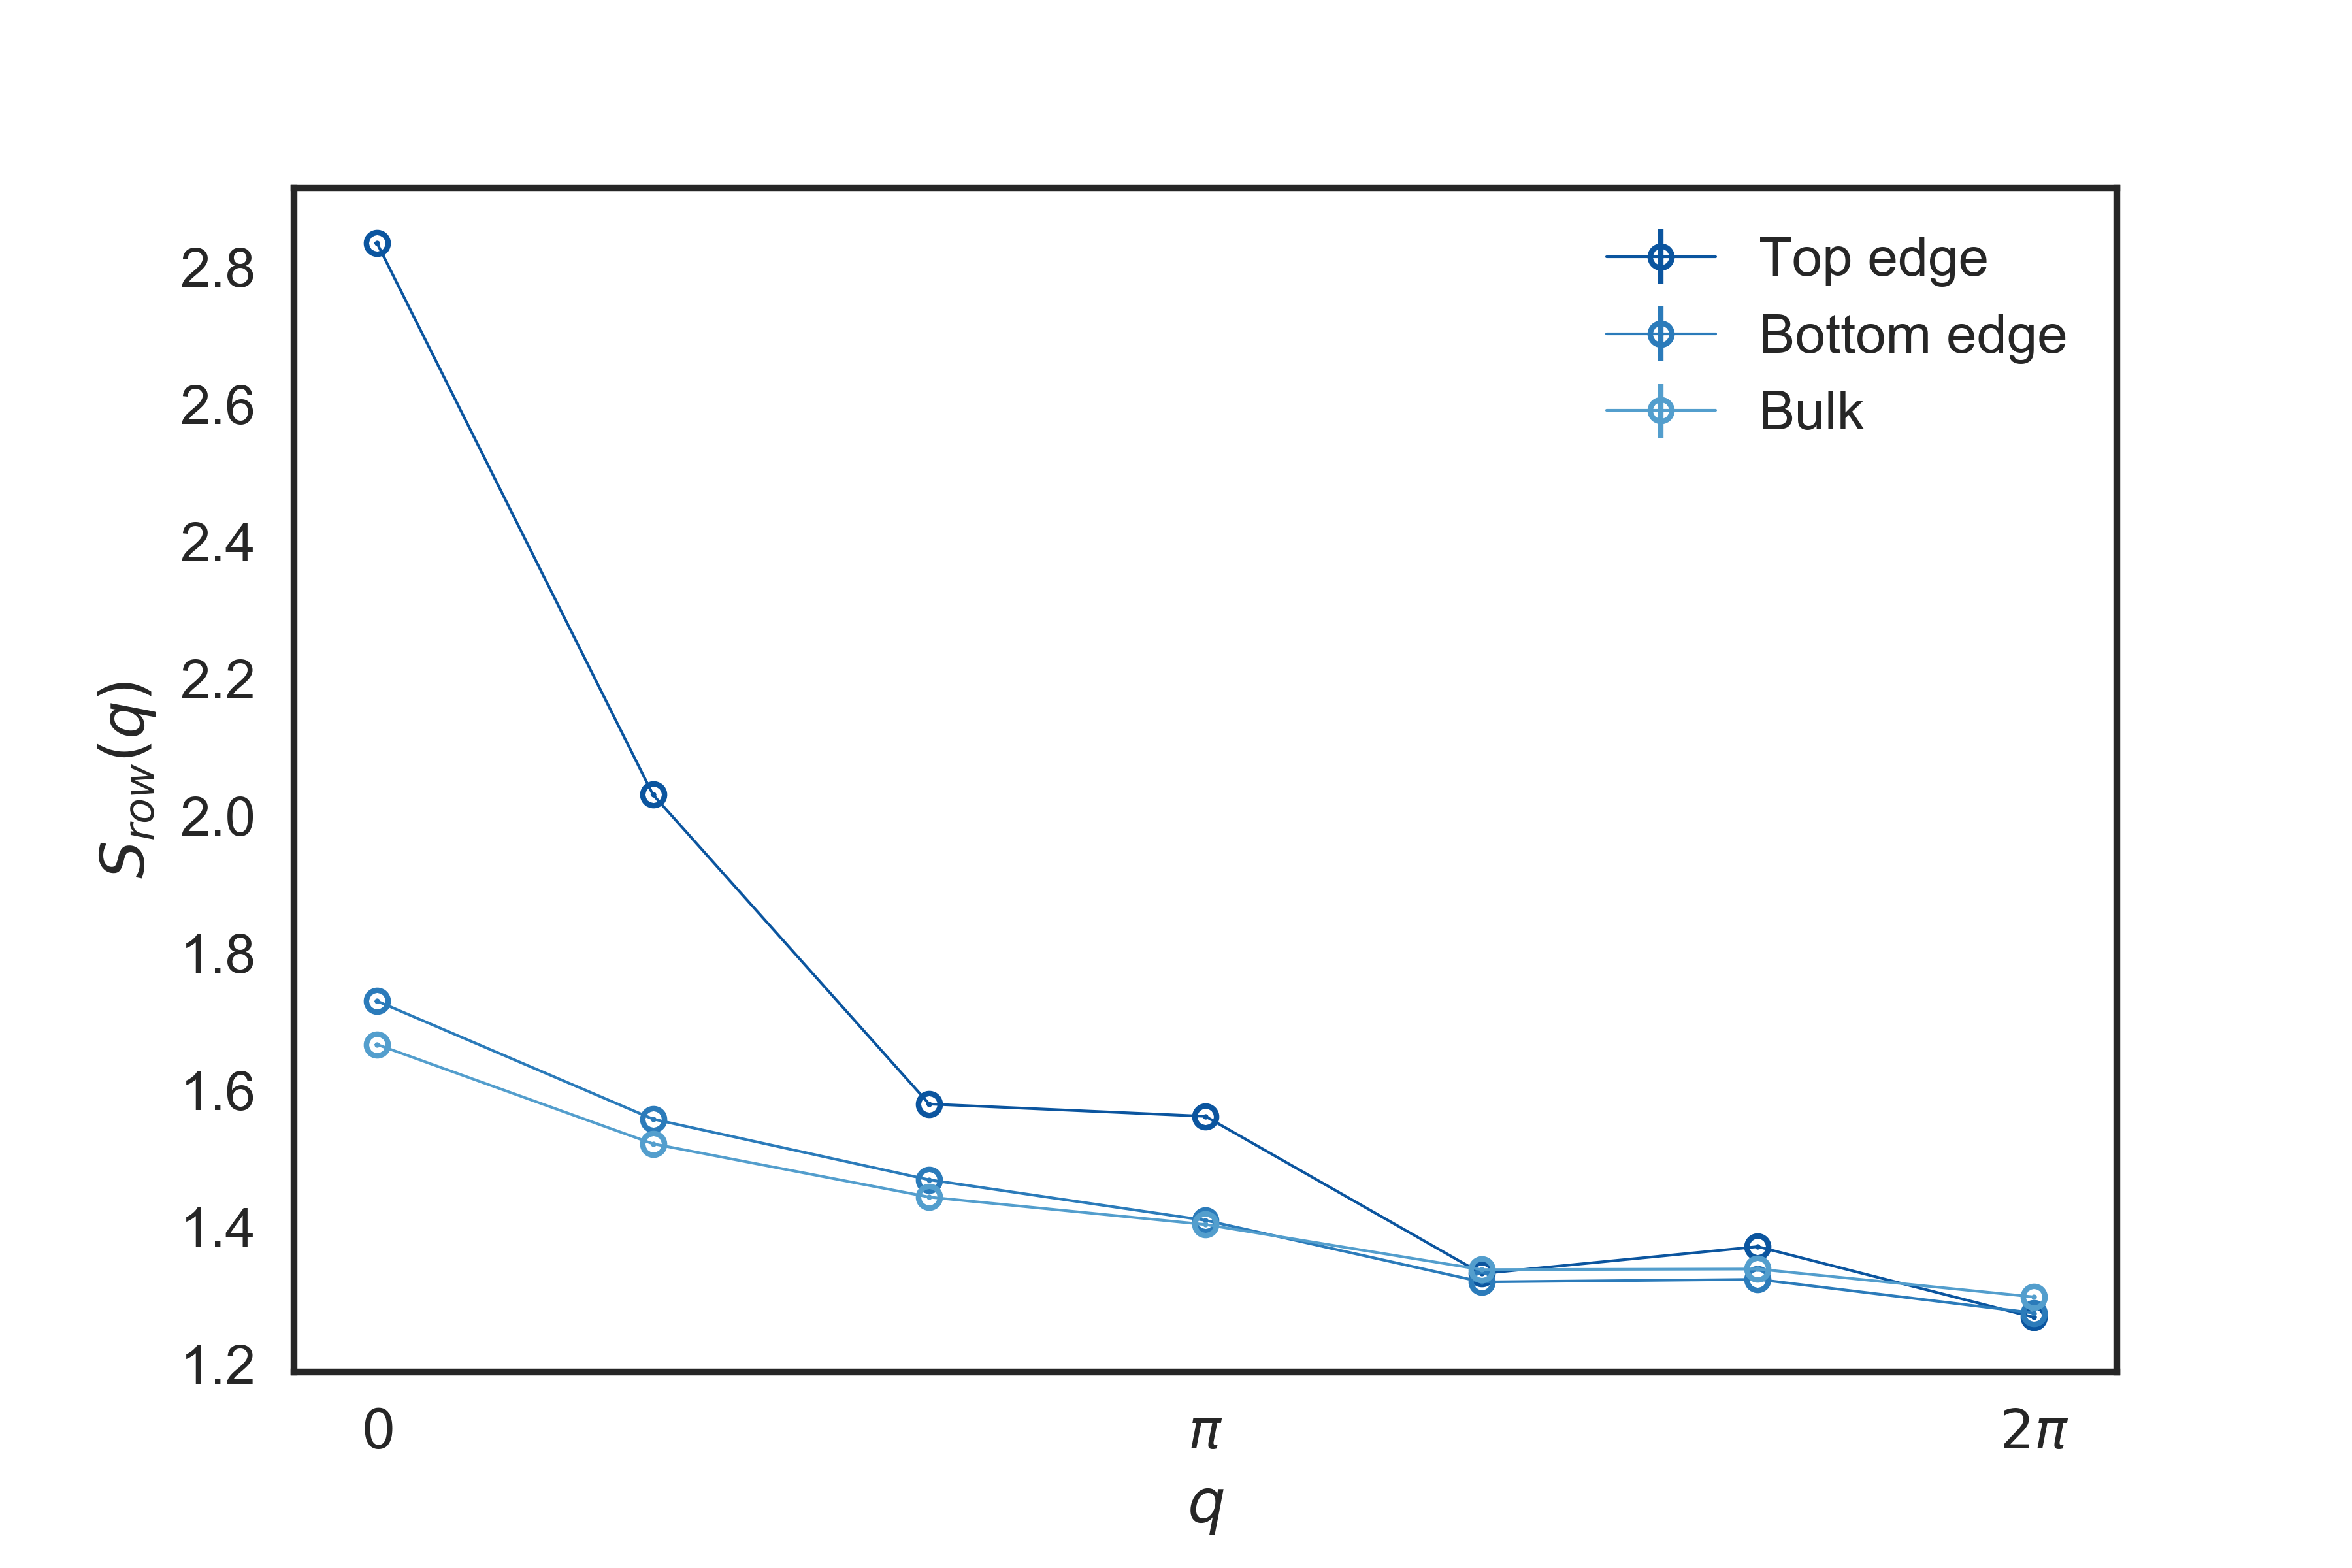
\includegraphics[scale = 0.55]{Applications/graphene-strain/edgeStFactor_Graphene.png}
	\caption[Magnetic structure factor $S(\bm q)$ for a strained graphene nanoribbon: bulk and edges.]{Magnetic structure factor $S(\bm q)$ for a strained graphene nanoribbon: total, i.e. bulk + edges (left) and edges compared with the innermost row of the bulk (right).}
	\label{fig:edgeStFactor}
\end{figure}
\begin{figure}[H]
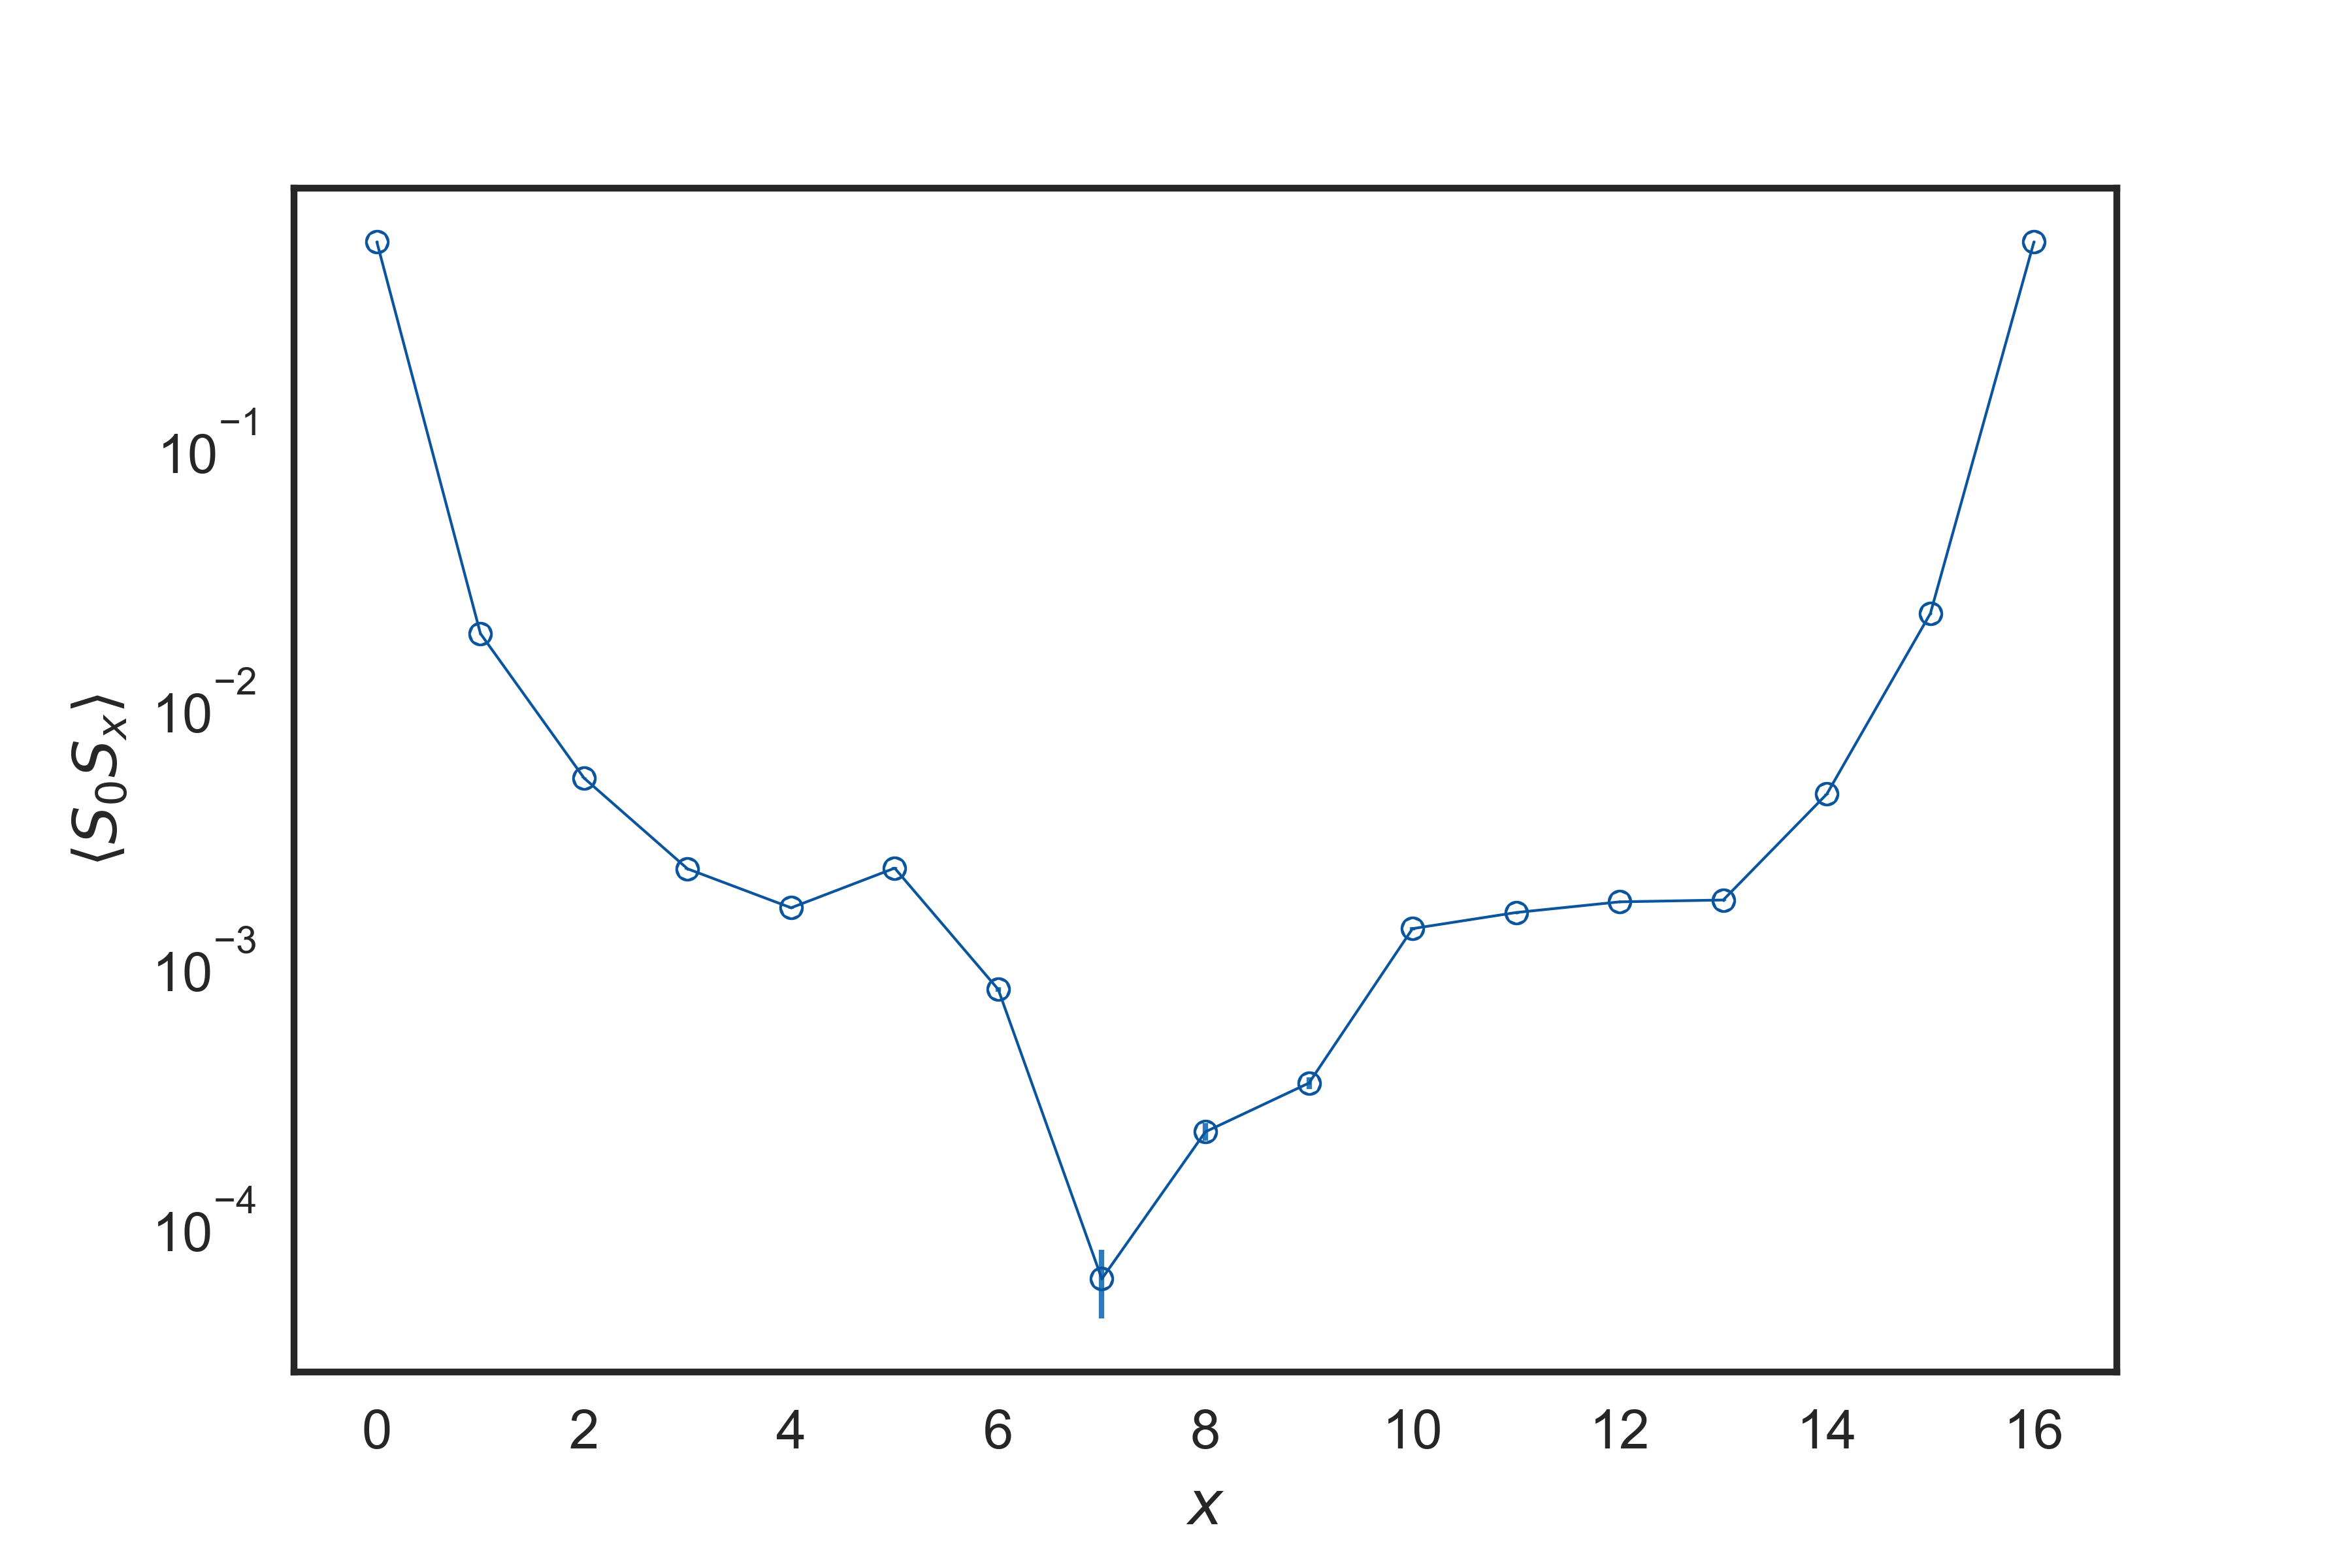
\includegraphics[scale = 0.55]{Applications/graphene-strain/LongitudinalProfile.png}
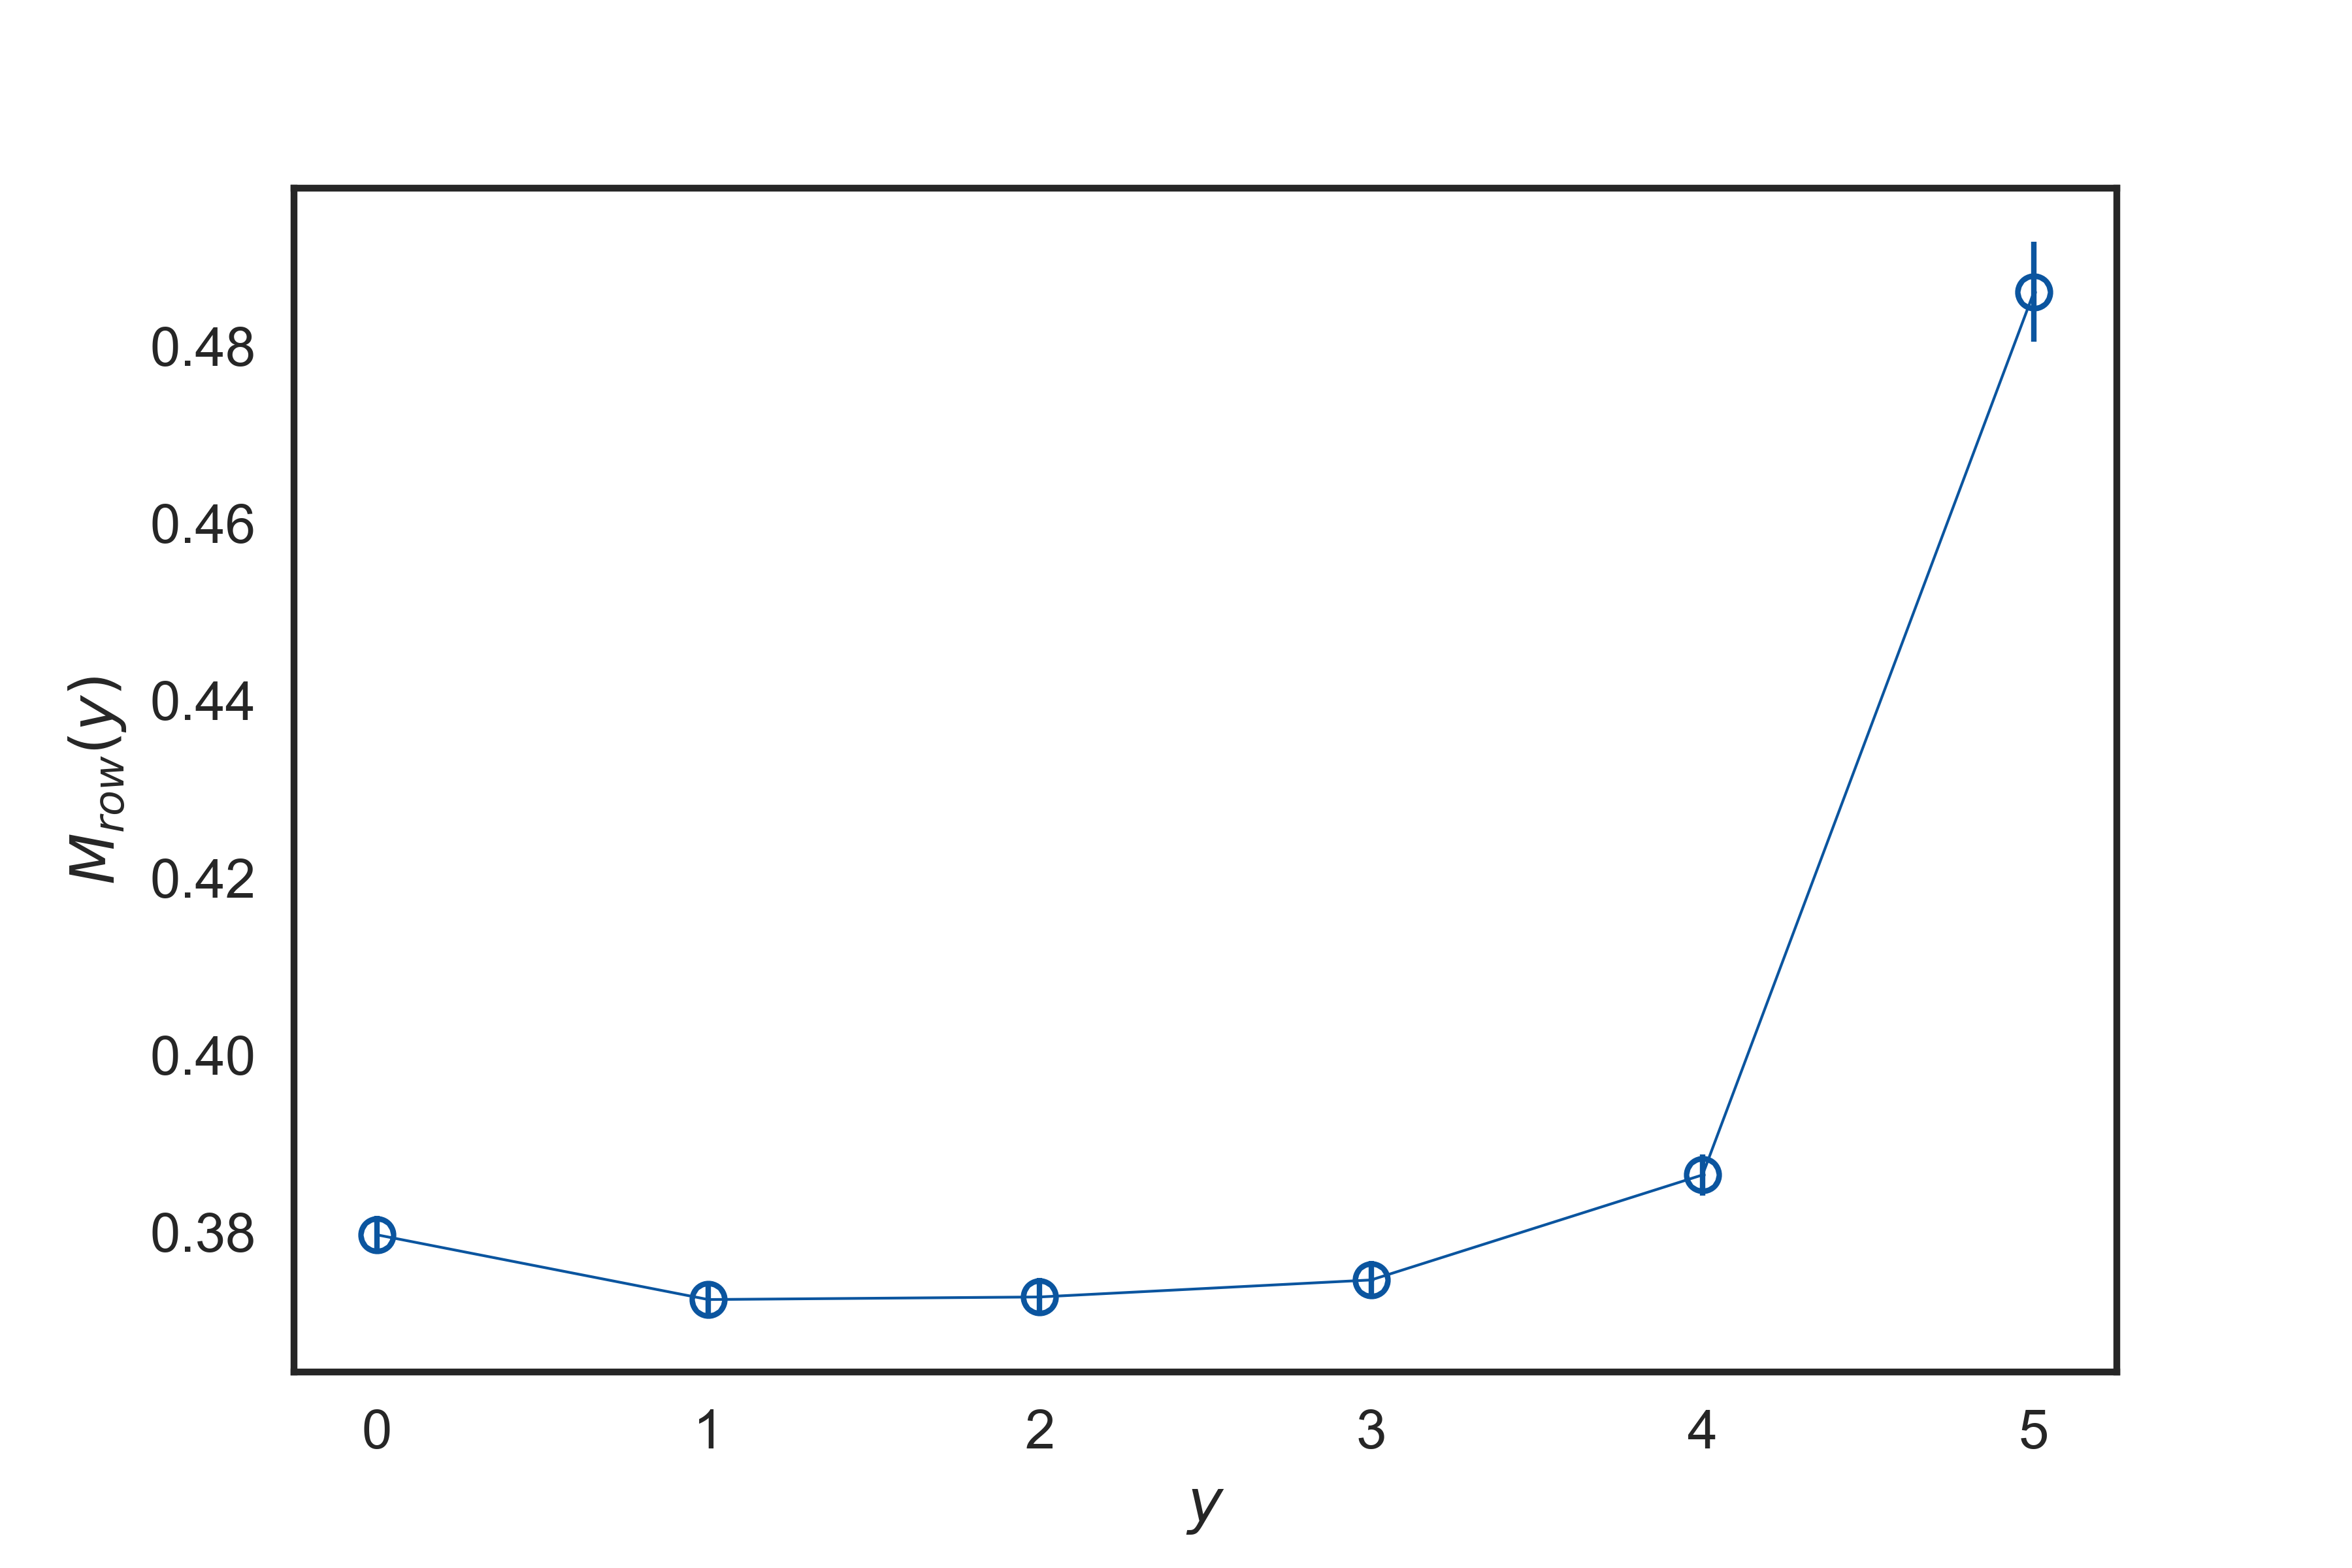
\includegraphics[scale = 0.55]{Applications/graphene-strain/order_parameter_Graphene.png}
	\caption[Spin-spin correlation function profile along the longitudinal direction $x$ of the ribbon. Magnetization parameter along each row, as a function of the transverse coordinate $y$.
	]{Left: Spin-spin correlation function profile along the longitudinal direction of the ribbon. Right: Magnetization parameter along each row, as a function of the transverse coordinate $y$, revealing the presence of magnetism localized at the edges.}
	\label{fig:longProf}
\end{figure}
We studied the phase transition to the ordered state we described in this section by carrying out many simulations at different temperatures.
By fitting the magnetic susceptibility at the edge $\chi_{edge} (\bm q = \bm 0)$ -which diverges at the transition - to the Curie-Weiss Law, we were able to find the critical temperature $(T_c = 0.017 \pm 0.003) t$, for the parameters $U = 3 t$, and $\Delta = 0.3 t$, a result which agrees with \cite{yang_strain-tuning_2017}.
Repeating this procedure for varying $U, \Delta$, we can obtain a complete phase diagram of the system.
\begin{figure}[H]
\hspace{0.2cm}
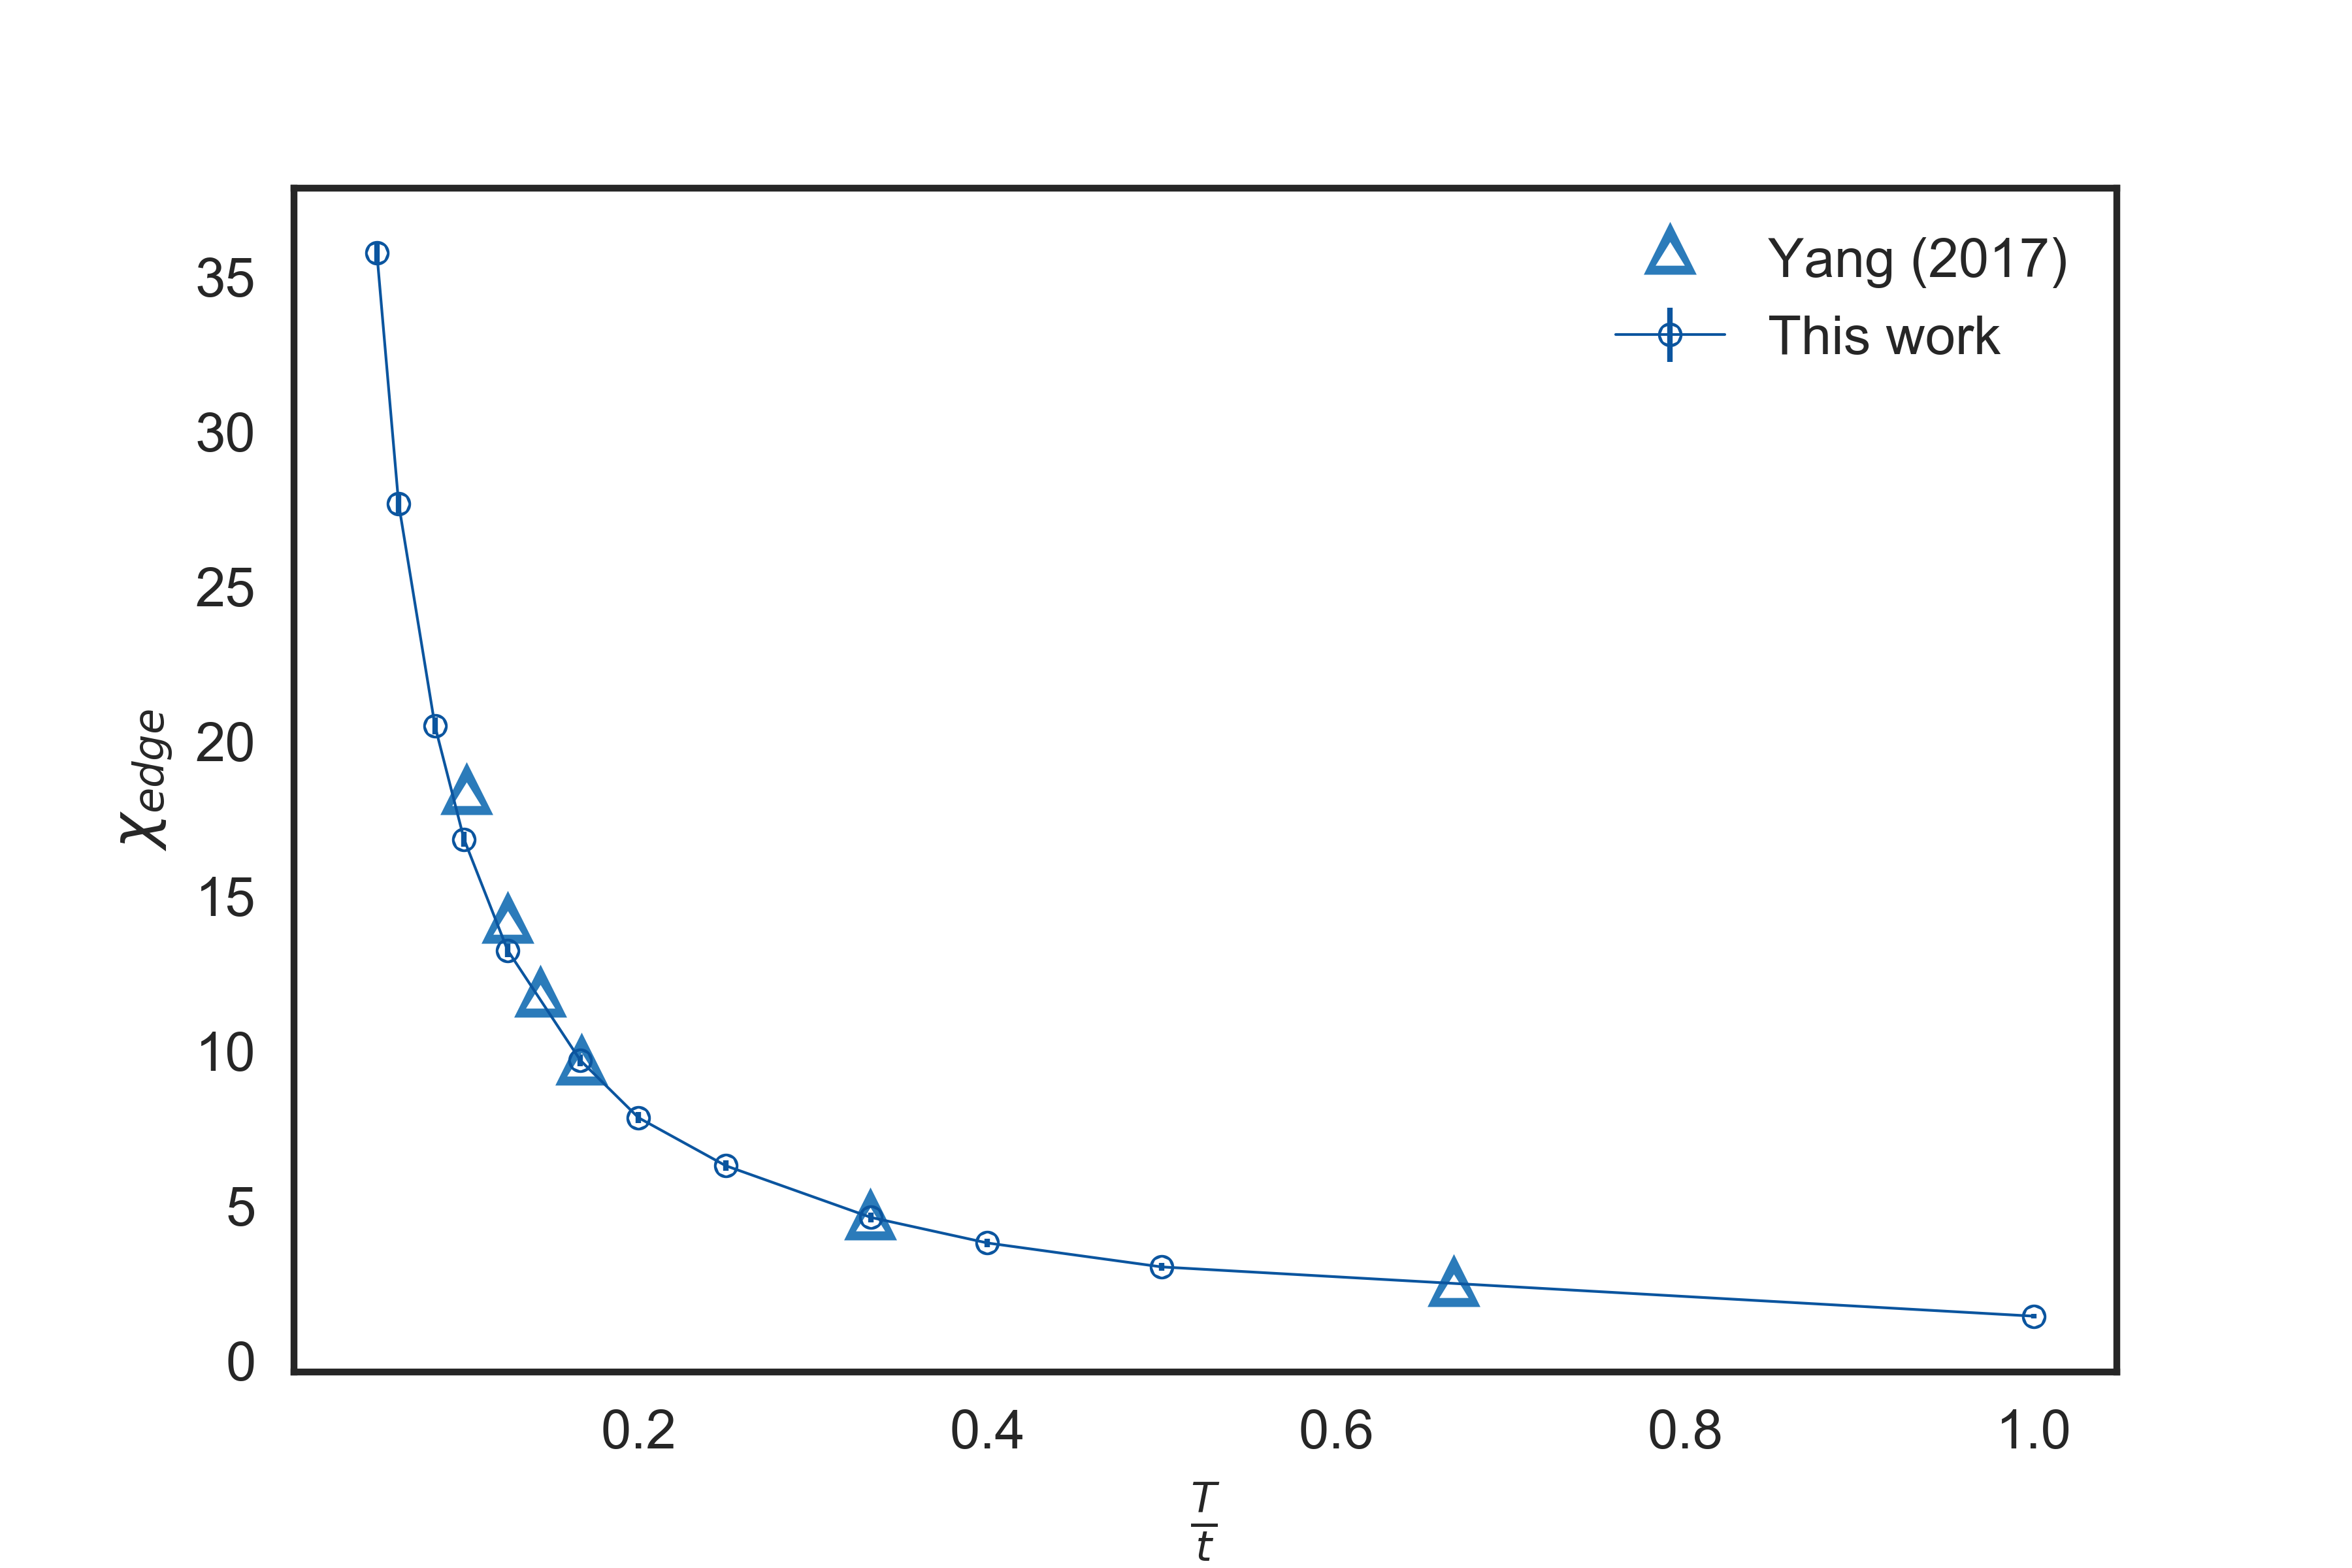
\includegraphics[scale = 0.55]{Applications/graphene-strain/chiTyang2017.png}
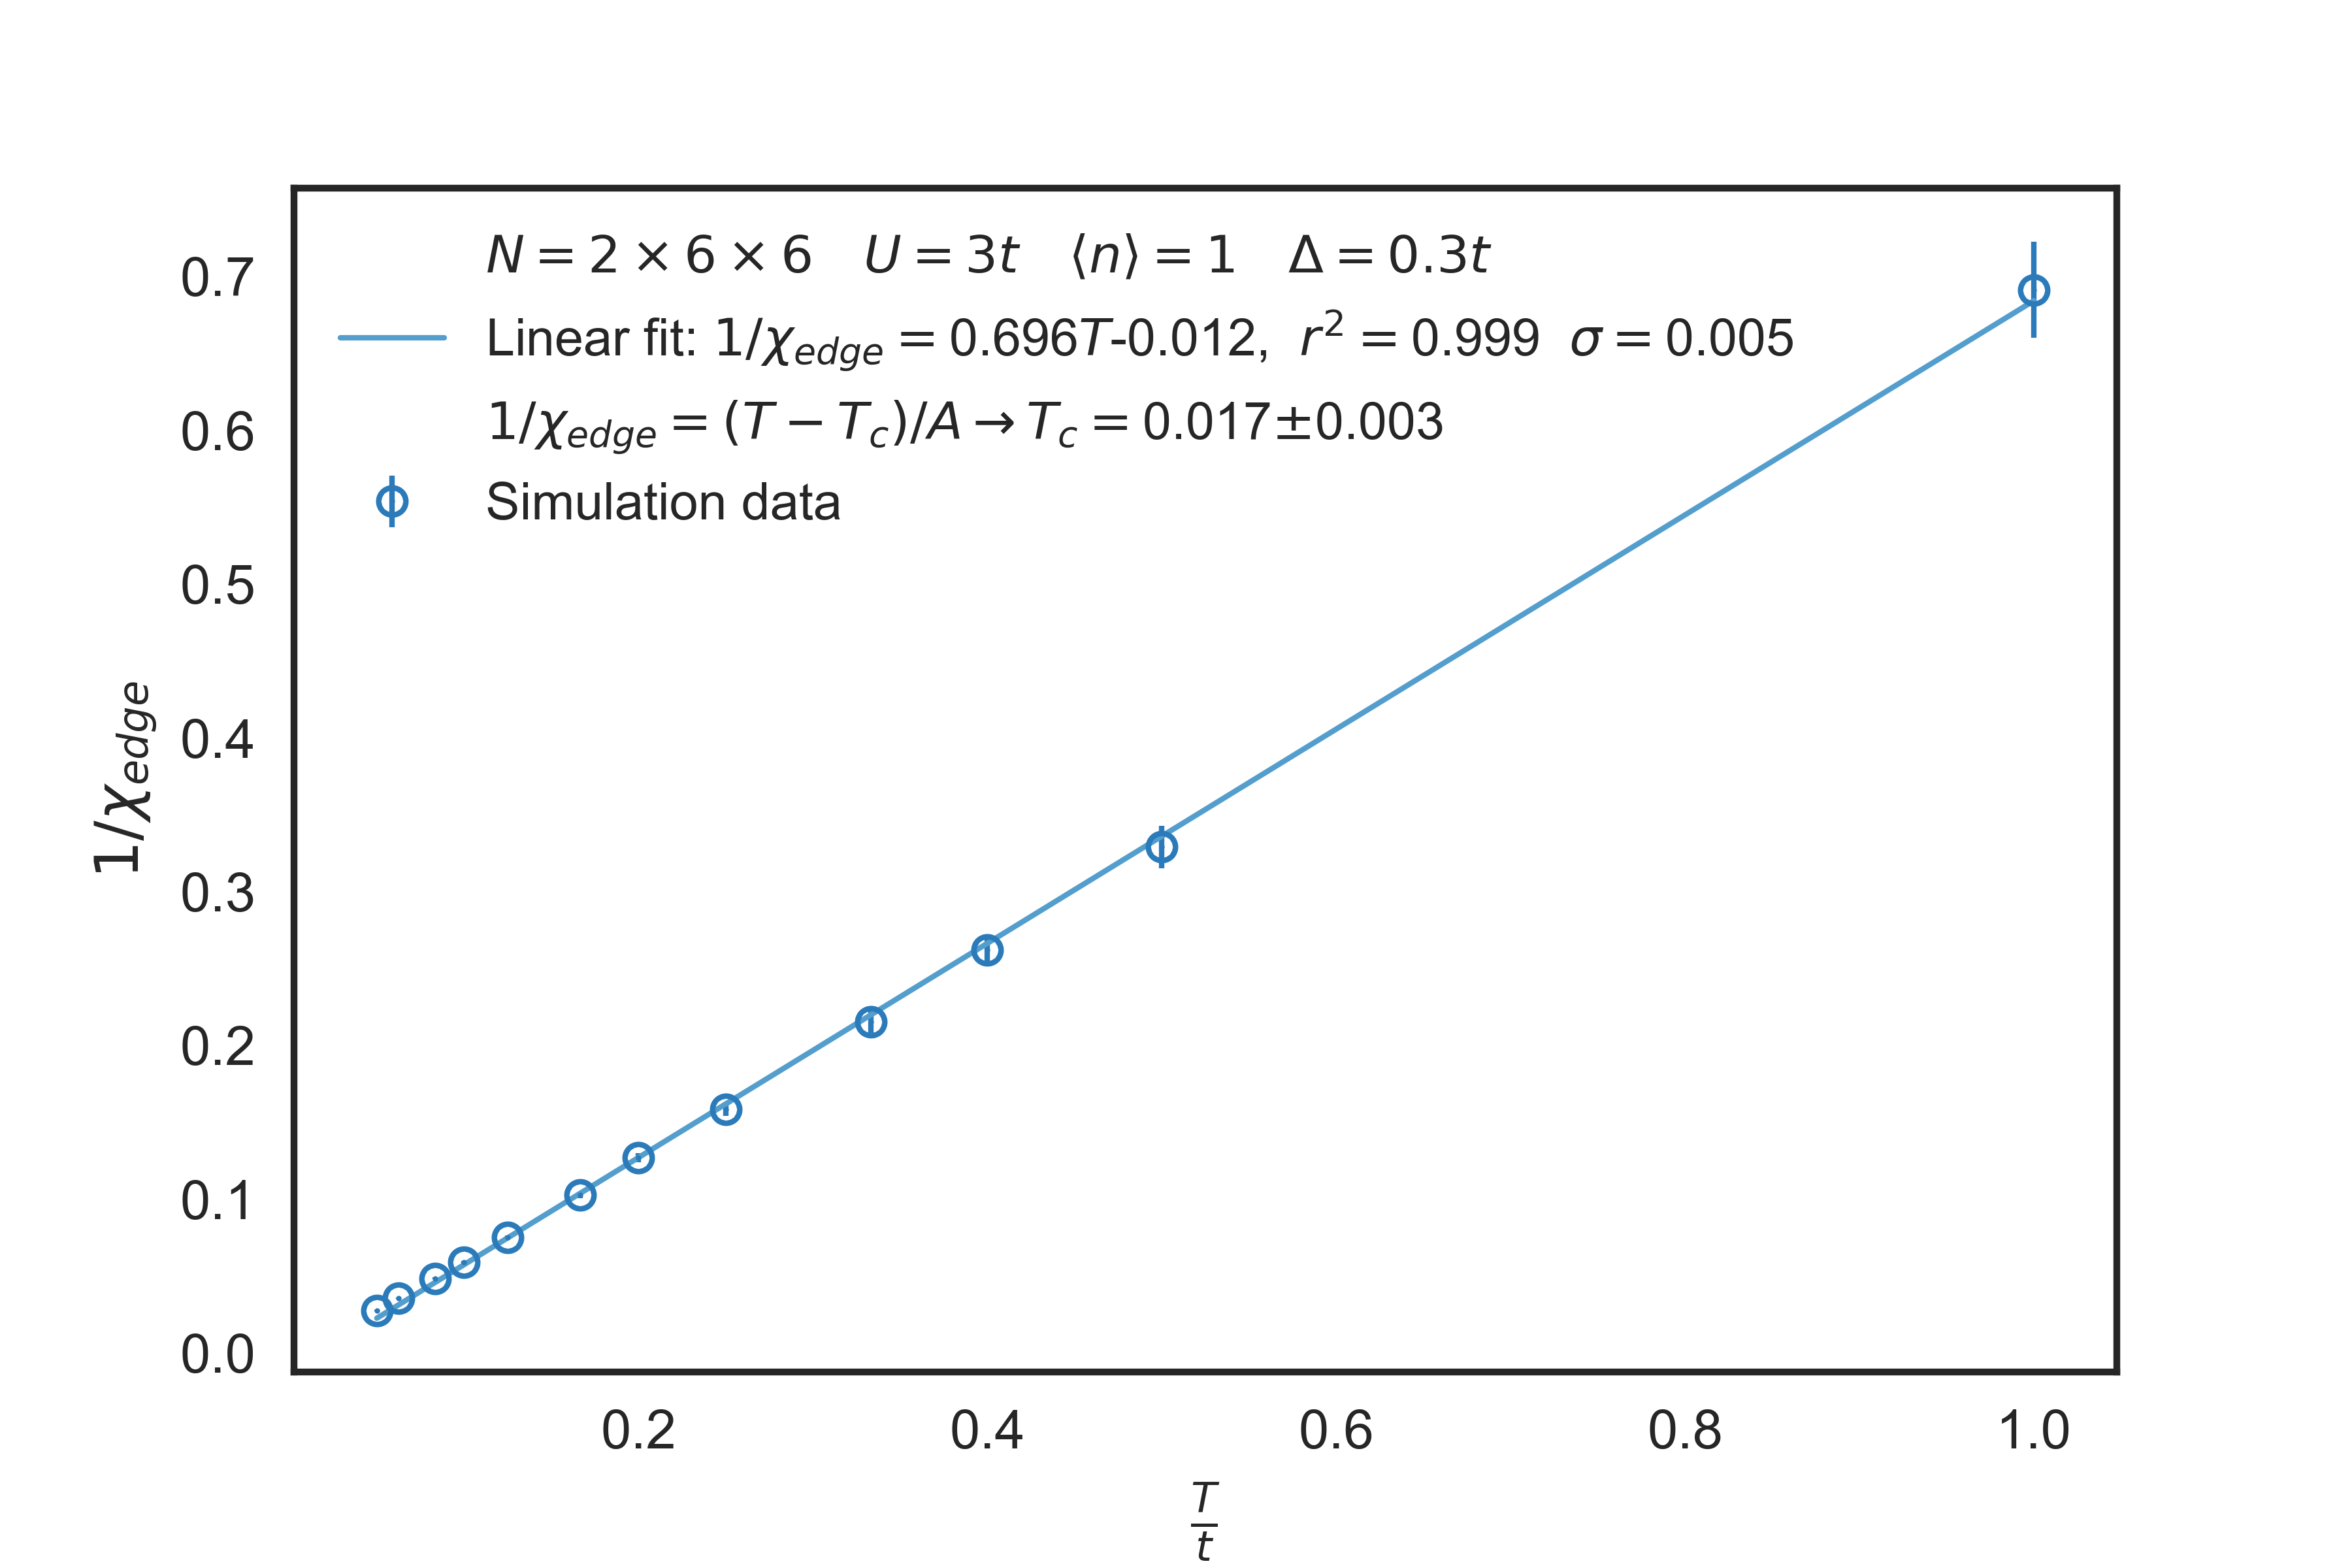
\includegraphics[scale = 0.55]{Applications/graphene-strain/fityang2017.png}
	\caption[Divergence of the edge susceptibility when approaching the critical temperature. Linear fit used to obtain the critical temperature of the transition to the edge-magnetized phase.]{Left: Divergence of the edge susceptibility when approaching the critical temperature. 
	Right: Linear fit used to obtain the critical temperature of the transition to the edge-magnetized phase.}
	\label{fig:chiFit}
\end{figure}

\subsection{\acp{TMD}}
\label{subsec:apTMD}

We start by approaching the \acs{TMDNR} problem at the mean field level.
Such a procedure is very useful to obtain a physical picture of the system's behavior.
In particular, at a given temperature, if there is a transition between a configuration with magnetic order, and a disordered one, there is a critical on-site interaction $U = U_c$ at which the transition occurs, and it can be estimated in mean field, and compared with the more precise, unbiased \acs{QMC} result (in both cases, we must sweep a certain range of interactions $U$ to look for ordering).
In the last sections we have demonstrated that we have the \say{tools} to carry out such a procedure.
Repeating the process for different temperatures, we can obtain a complete phase diagram.

In general, our mean field formulation would involve diagonalizing an $N \times N$ matrix at each step, where $N = N_{\text{orb}} N_x N_y$ is the size of the system times the number of orbitals.
However, since we consider \acs{PBC}s along the $x$-direction, we can partially diagonalize  the Hamiltonian analytically, reducing the size of the matrix to be diagonalized to $N_{\text{orb}} N_y \times N_{\text{orb}} N_y$, where $N_y$ is the width of the ribbon, i.e. the number of $\text{M}\text{X}_2$ formula units.
Consider the spinless 3-band tight binding model, with unit lattice constant:
\begin{equation}
\begin{split}
\mathcal{H}_0 &= \sum_{\substack{m, n \\ \alpha, \beta}} \bigg( c_{m,n, \alpha}^\dagger t_{\alpha\beta}^0 c_{m, n, \beta} + \delta_{0, N_x}  c_{m,n, \alpha}^\dagger t_{\alpha\beta}^1 c_{m+1, n, \beta} + \delta_{-\sqrt{3}/2, (N_y -1)\sqrt{3}/2}  c_{m,n, \alpha}^\dagger t_{\alpha\beta}^4 c_{m-1, n, \beta} \\
& + \delta_{0, N_m} \delta_{-1, (N_y -1)\sqrt{3}/2} c_{m+1/2,n-\sqrt{3}/2, \alpha}^\dagger t_{\alpha\beta}^2 c_{m, n, \beta} + \delta_{-1, (N_y -1)\sqrt{3}/2} c_{m-1/2,n-\sqrt{3}/2, \alpha}^\dagger t_{\alpha\beta}^3 c_{m, n, \beta} \\
& + \delta_{N_y\sqrt{3}/2, 0} c_{m+1/2,n+\sqrt{3}/2, \alpha}^\dagger t_{\alpha\beta}^6 c_{m, n, \beta} + \delta_{-1, N_x -1} \delta_{N_y\sqrt{3}/2, 0} c_{m-1/2,n+\sqrt{3}/2, \alpha}^\dagger t_{\alpha\beta}^5 c_{m, n, \beta} \bigg)
\end{split}
\end{equation}

Fourier transforming along $m$: $c_{m, n, \alpha} = \frac{1}{\sqrt{N_x}}\sum_{k} e^{-i k m } c_{k, n, \alpha} $, with $k = \frac{2\pi}{N_x} \{ -\frac{N_x}{2} + 1, -\frac{N_x}{2}, ..., \frac{N_x}{2} \}$:
\begin{equation}
\begin{split}
\mathcal{H}_0 &= \sum_{ \substack{k, y \\ \alpha, \beta} } \bigg( c_{k, y, \alpha}^\dagger (t_{\alpha \beta}^0  + e^{ik} t_{\alpha \beta}^1 + e^{-ik} t_{\alpha \beta}^4 )  c_{k, y, \beta} + \delta_{-1, N_y -1} c_{k, y - 1, \alpha}^\dagger ( e^{ik/2} t_{\alpha \beta}^2 + e^{-ik/2} t_{\alpha \beta}^3 ) c_{k, y, \beta} \\
& + \delta_{N_y, 0} c_{k, y, \alpha}^\dagger ( e^{ik/2} t_{\alpha \beta}^6 + e^{-ik/2} t_{\alpha \beta}^5 ) c_{k, y+1, \beta} \bigg) , \,\, \text{with} \, y \, \text{defined as in Fig.(4.1)}
\end{split}
\end{equation}
leading to a tridiagonal block $3 N_y \times 3 N_y$ hopping matrix $\bm H (k)$ with three different types of matrix elements: $\bm h_1 = \bm H_{y,y}$, $\bm h_2 = \bm H_{y,y-1}$, $\bm h_2^\dagger = \bm H_{y, y+1}$.
\begin{equation}
[ H_{(\alpha y) (\beta y')} (k) ] = 
\begin{pmatrix}
\bm h_1 & \bm h_2^\dagger & & & \\
\bm h_2 & \bm h_1 & \bm h_2^\dagger & & \\
& \bm h_2 & \bm h_1 & \ddots & \\
& & \ddots & \ddots & \bm h_2^\dagger \\
& & & \bm h_2 & \bm h_1
\end{pmatrix}, \, 
\bm h_1 = 
\begin{pmatrix}
\varepsilon_1 + 2 t_0 \cos k & 2 i t_1 \sin k & 2 t_2 \cos k \\
-2 i t_1 \sin k & \varepsilon_2 + 2 t_{11} \cos k & 2 i t_{12} \sin k \\
2 t_2 \cos k& -2 i t_{12} \sin k & \varepsilon_2 + 2 t_{22} \cos k \\
\end{pmatrix}
\end{equation}
\begin{equation*}
\bm h_2 =
\begin{pmatrix}
2 t_0 \cos ( k / 2 ) & i \sin ( k / 2 ) \bigg( t_1 - \sqrt{3} t_2 \bigg) & - \cos (k /2 ) \bigg( \sqrt{3} t_1 + t_2 \bigg) \\
-i \sin ( k / 2 ) \bigg(t_1 + \sqrt{3} t_2 \bigg) & \frac{1}{2} \cos (k / 2) \bigg( t_{11} + 3 t_{22} \bigg) & -i \sin (k / 2) \bigg( \frac{\sqrt{3}}{2} (t_{11} -  t_{22} ) + 2 t_{12} \bigg) \\
\cos ( k / 2) \bigg( \sqrt{3} t_1 - t_2 \bigg) & -i \sin (k / 2) \bigg( \frac{\sqrt{3}}{2} ( t_{11} - t_{22} ) - 2 t_{12} \bigg) & \frac{1}{2} \cos (k / 2) \bigg( 3 t_{11	} + t_{22} \bigg)
\end{pmatrix}
\end{equation*}
\begin{figure}[H]
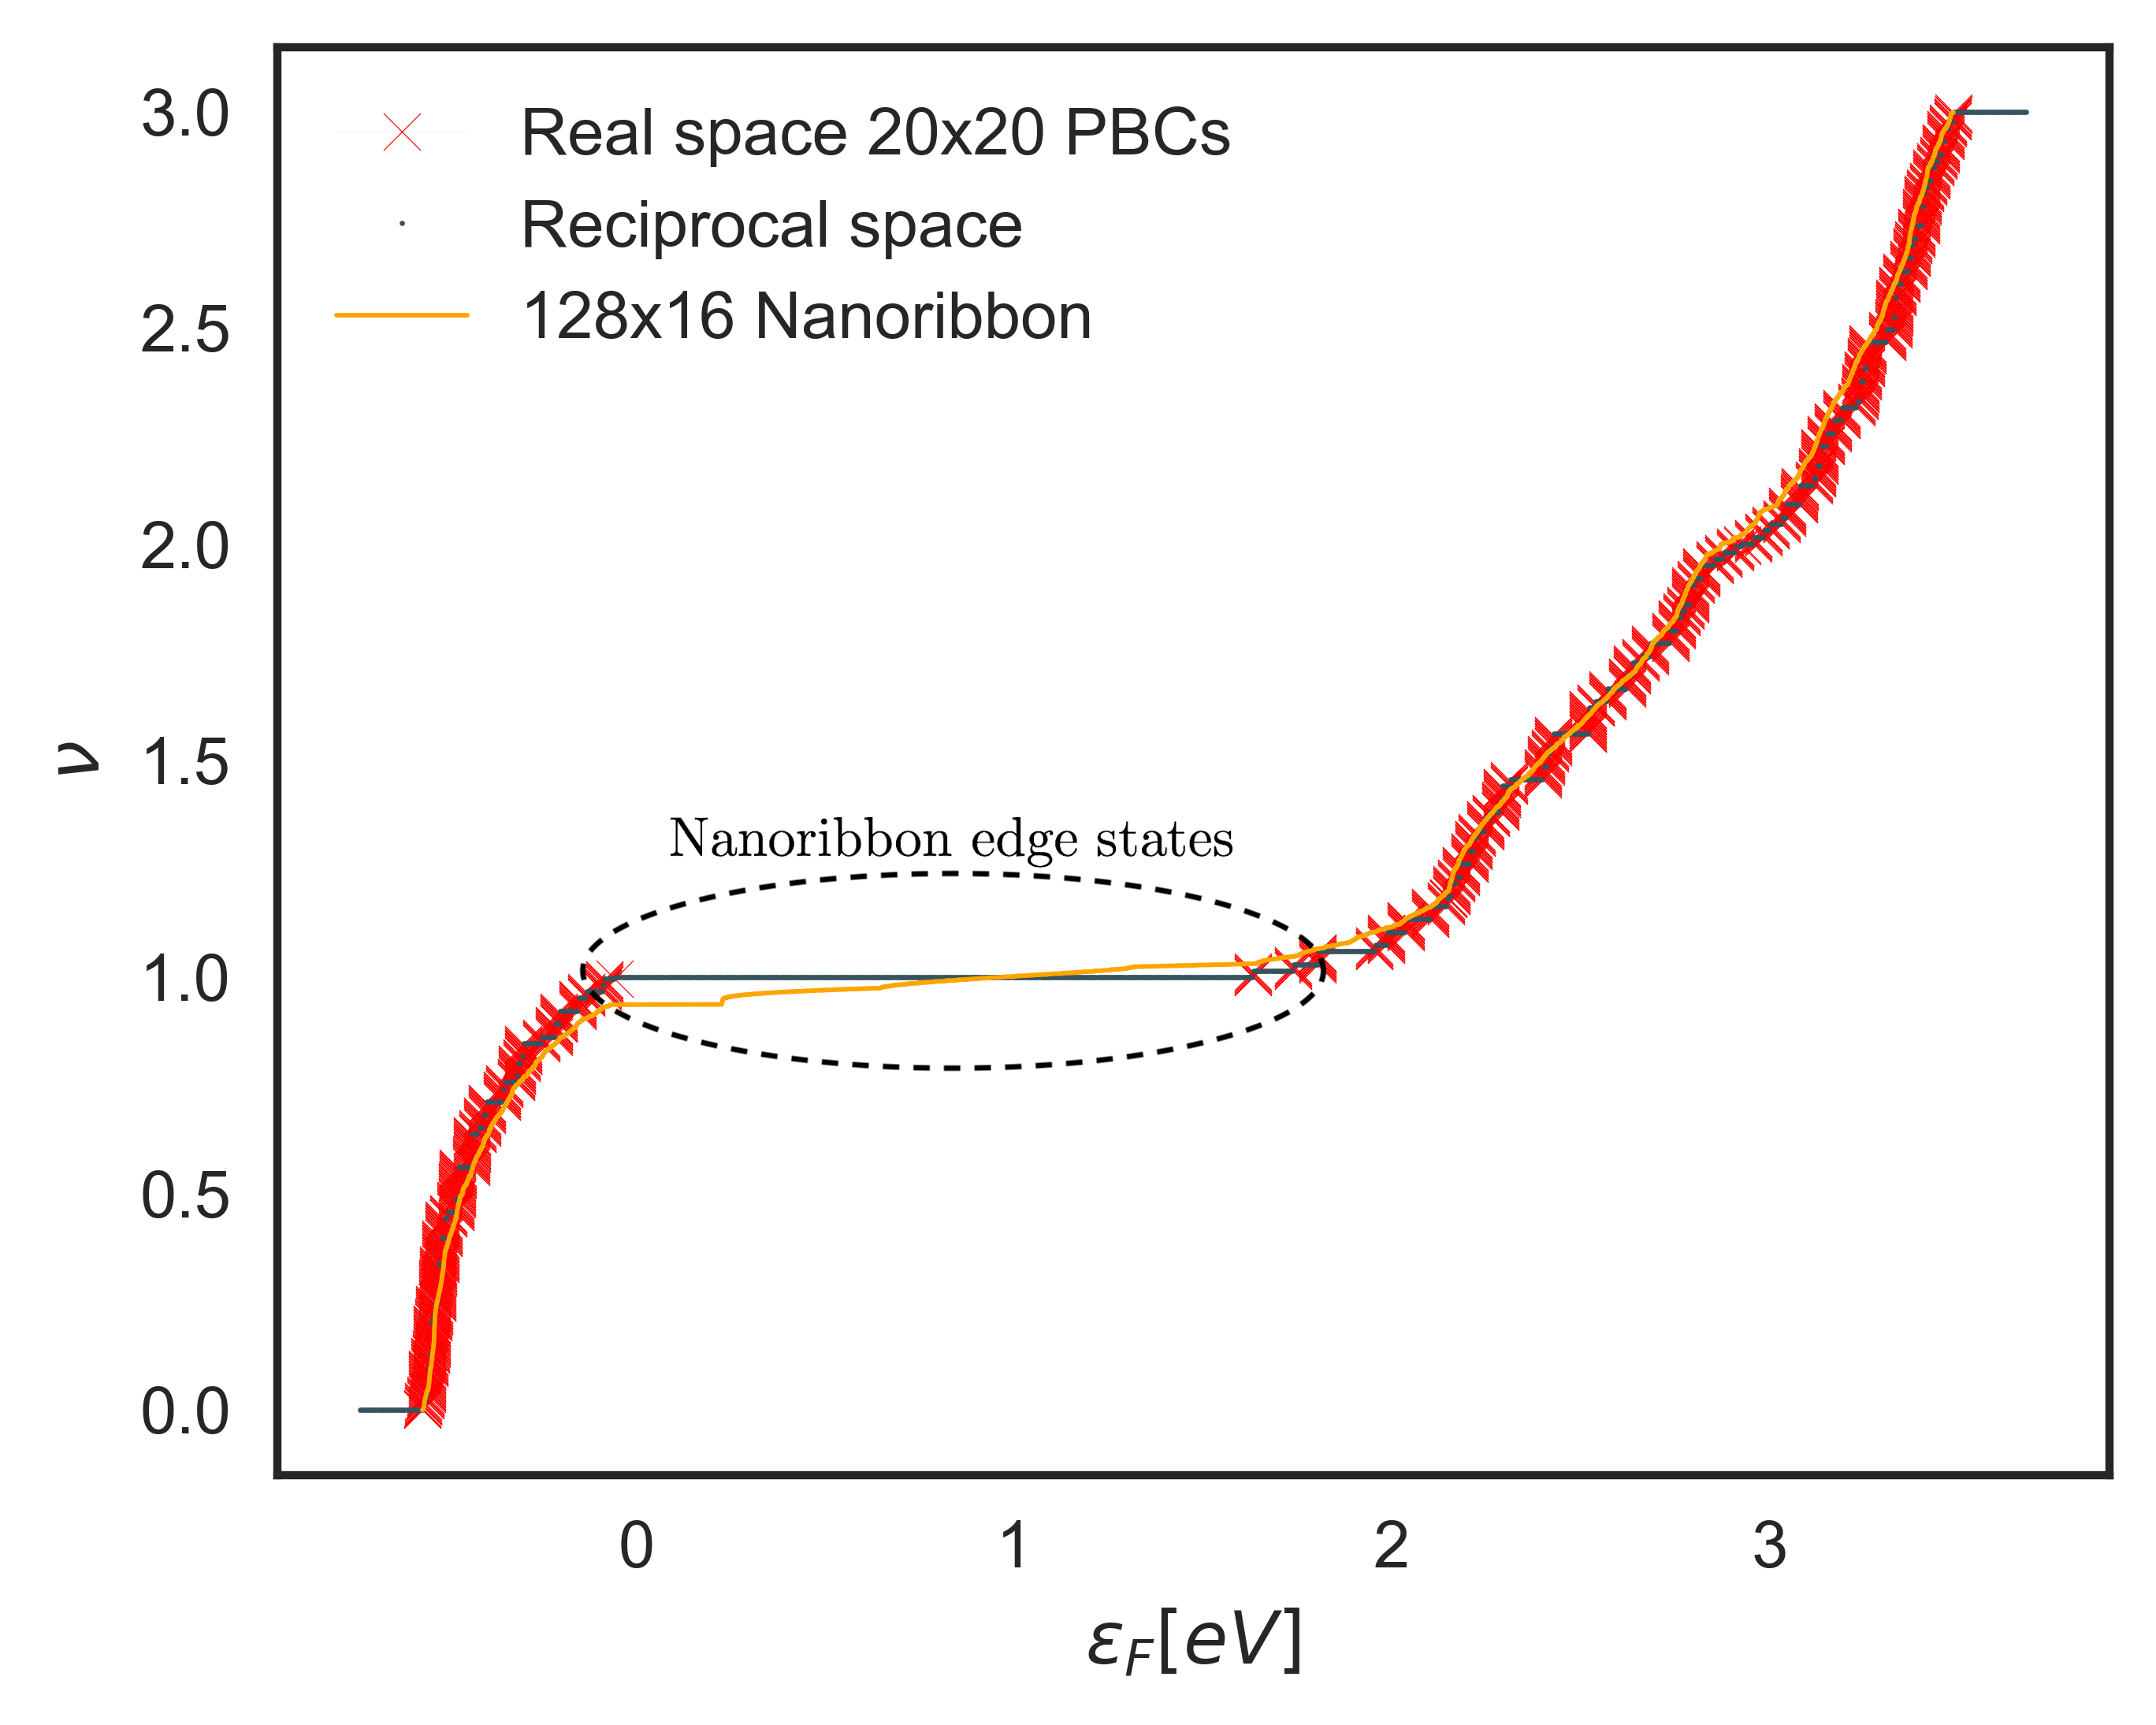
\includegraphics[scale=0.55]{Applications/fillingVsE.png}
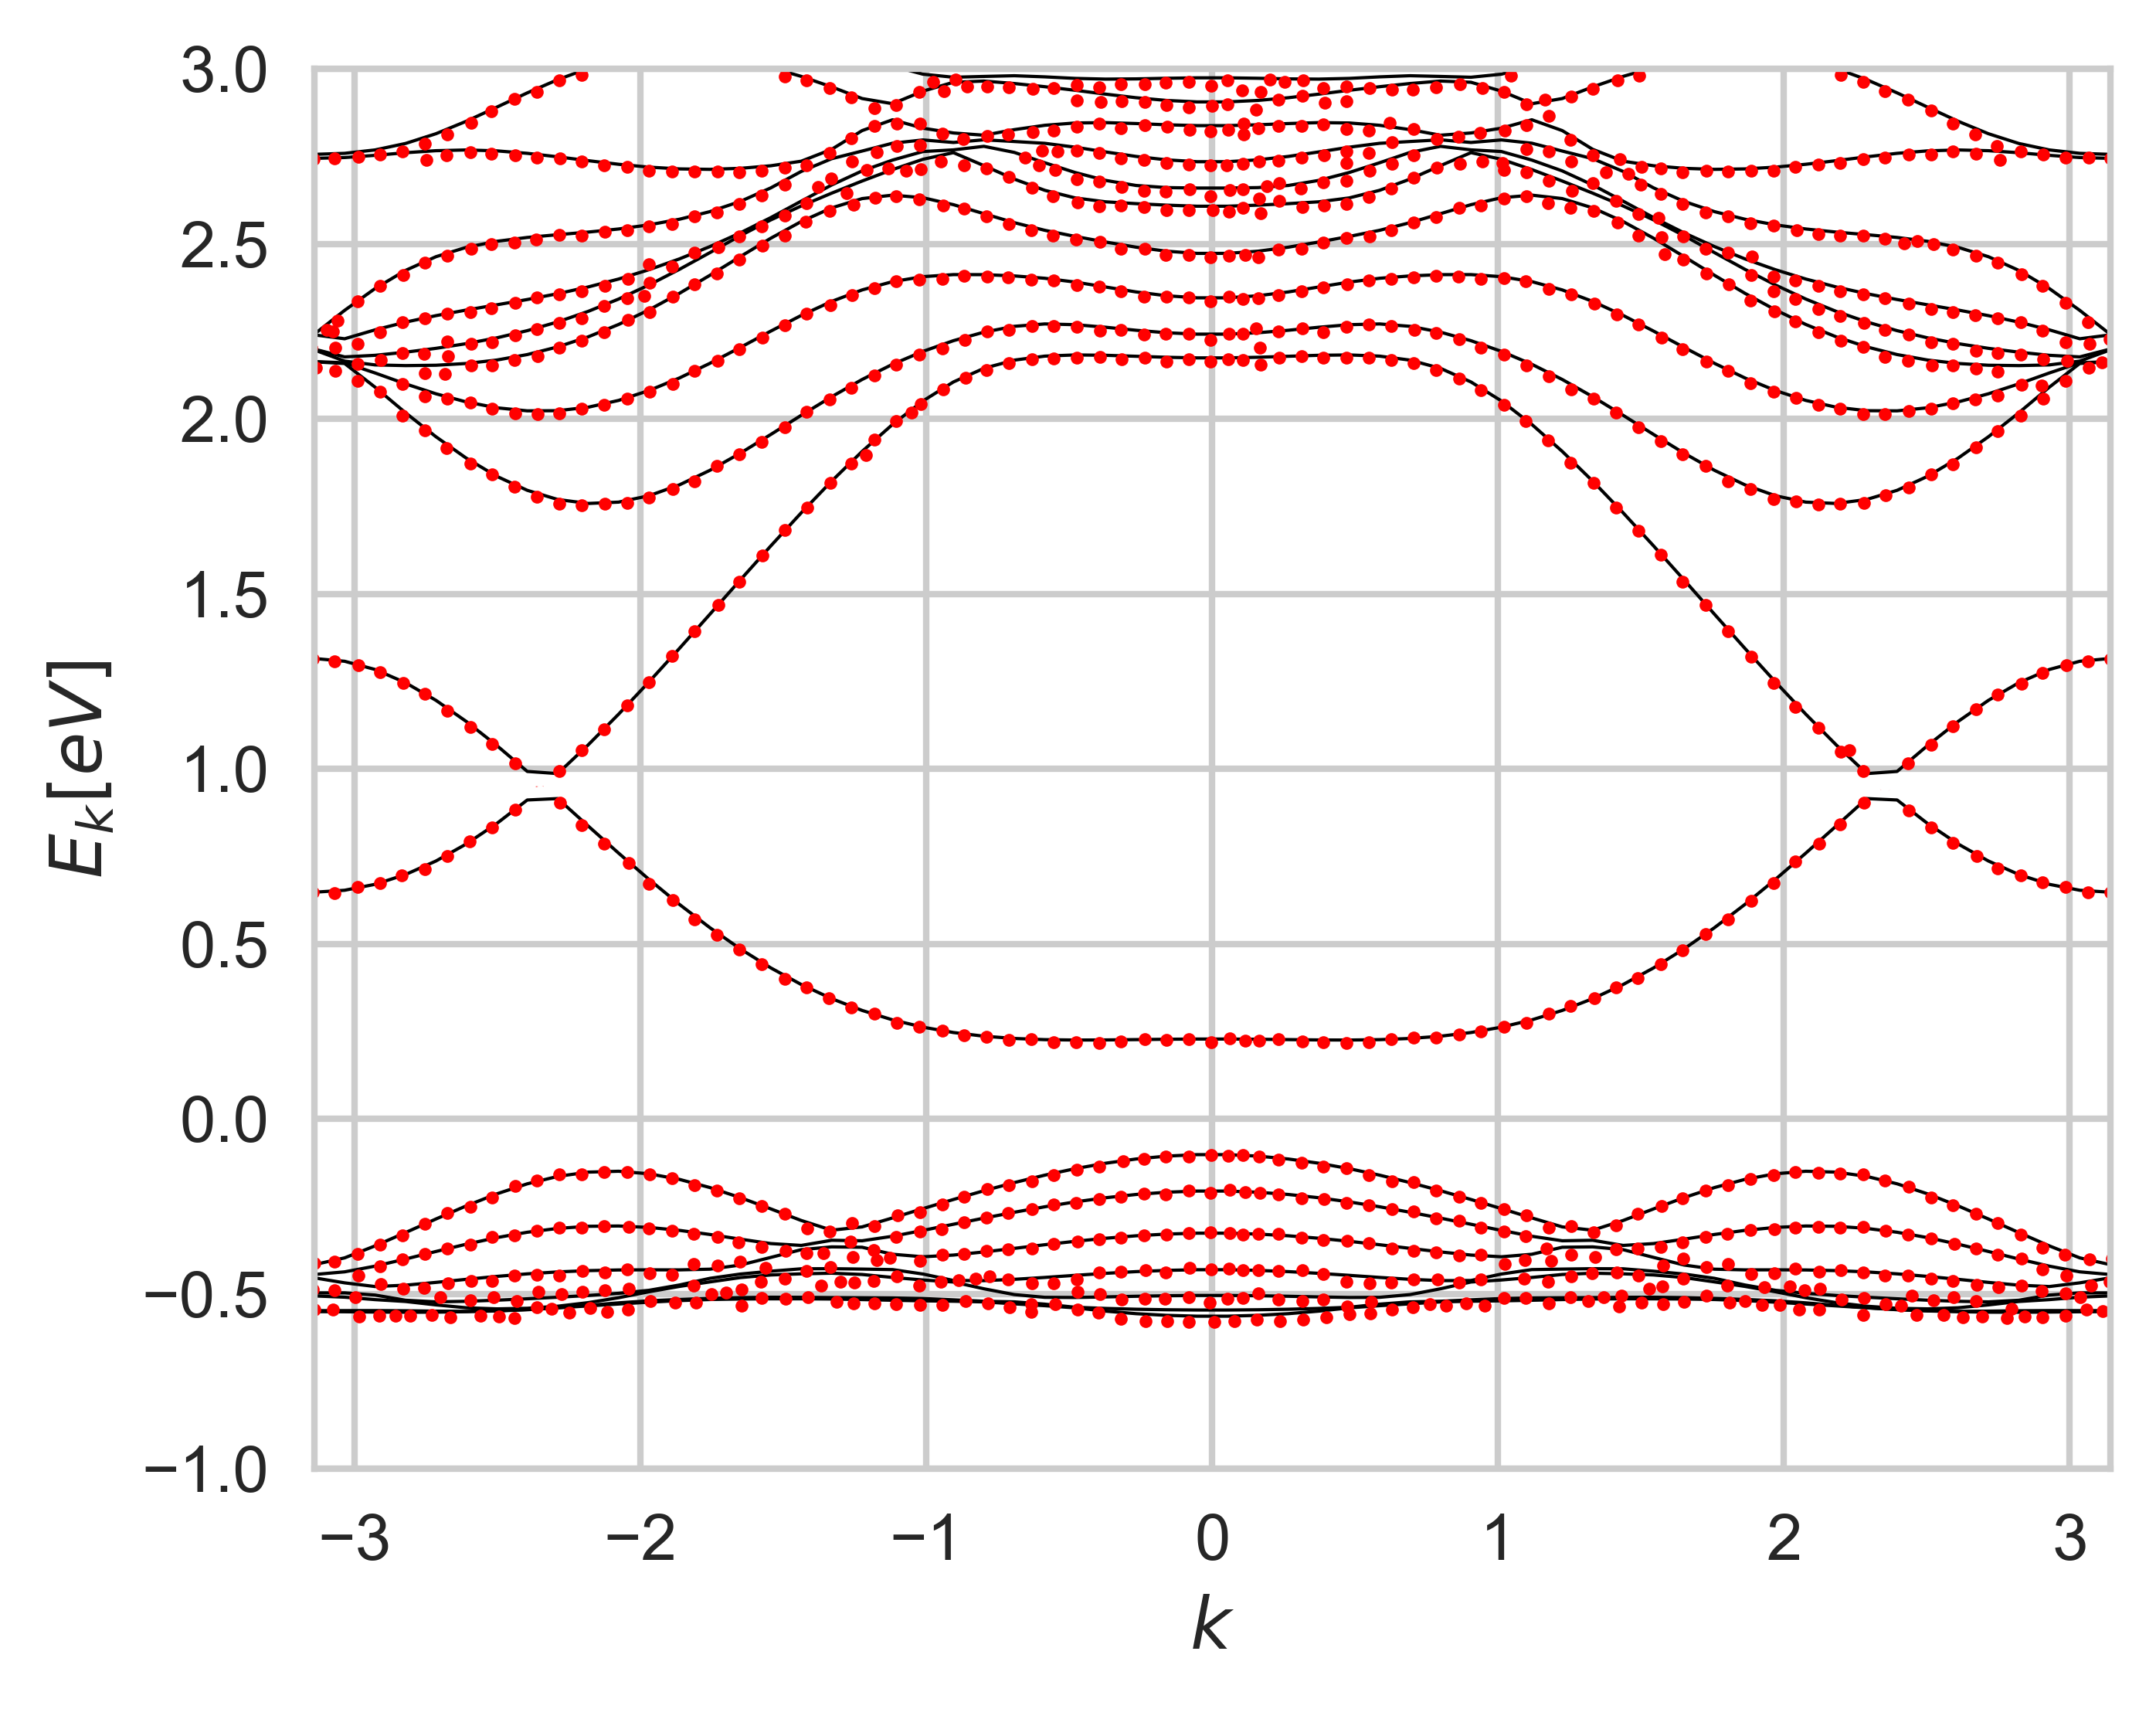
\includegraphics[scale=0.55]{Applications/BandStructureNanoribbonTMD.png}
	\caption[Filling $\nu$ as a function of the Fermi energy $\varepsilon_F$ for a \acs{TMD} monolayer and a nanoribbon. $\text{Mo}\text{S}_2$.  \acs{TMDNR} band structure obtained by the 3-band model.]{Left: Filling $\nu$ as a function of the Fermi energy $\varepsilon_F$ for a system with \acp{PBC}, as computed by diagonalizing the input matrix of our code, and by the hopping matrix in $\bm k$-space. Comparison between the fillings of a nanoribbon and a periodic system.
	For the nanoribbon, edge states appear on the gap of the periodic system.
	Right: 3-band model $\text{Mo}\text{S}_2$ zigzag edged nanoribbon energy bands (red dots and orange curve), for $N_y = 8$, using the GCA parameters. The first principles bands show the contribution from orbitals that are not considered in the 3-band model (blue:  $d_{z^2}$, $d_{xy}$, $d_{x^2-y^2}$, green: others). The 3-band model reproduces the bands that correspond to the orbitals taken into account reasonably (1 and 2 correspond to the edge states from the $d_{z^2}$, $d_{xy}$, $d_{x^2-y^2}$ orbitals of the $\text{Mo}$ atoms, while 3 and 4 correspond to the $d_{yz}$ orbital at the $\text{Mo}$-terminated edge, and $p_{y, z}$ orbitals from the $\text{S}$-terminated edge, and are not taken into account in the 3-band model).\cite{liu_three-band_2013}.}
	\label{fig:fillingVsE}
\end{figure}

By applying our mean field approach to solve the 3-band model with Hubbard-type interactions, we obtain solutions that are independent of $x$, which motivates us to reduce the number of MF parameters by choosing a translationally invariant ansatz.
This is equivalent to taking $\left\langle n_{x, y,\alpha, \sigma}\right\rangle = \left\langle n_{y,\alpha, \sigma}\right\rangle  \forall x$ ($6 N_y$ parameters).
By reducing the number of parameters, convergence is facilitated, which allows us to evaluate whether the solution of Fig.(\ref{fig:nanoGraphVsTMD}) is robust, i.e. whether it corresponds to a metastable or not.
The mean field form of the interaction term with the reduced number of parameters changes, implying that the self-consistent relation of Eq.(\ref{eq:selfConsistent}) from which the local densities are computed changes as well.
\begin{equation}
\mathcal{H}_{\text{MF}} = \mathcal{H}_0 + \mathcal{H}_1 + \mathcal{C} , \,\text{where} \,\, \mathcal{H}_1 = U \sum_{m, n, \alpha}  \sum_\sigma n_{\substack{m, \sigma \\ n, \alpha}} \big\langle n_{\substack{m, -\sigma \\ n, \alpha}} \big\rangle  , \,\, \mathcal{C} = -U  \sum_{m, n, \alpha} \big\langle n_{\substack{m, \uparrow \\ n, \alpha}} \big\rangle \big\langle n_{\substack{m, \downarrow \\ n, \alpha}} \big\rangle
\end{equation}
\begin{equation}
\begin{split}
\mathcal{H}_1 + \mathcal{C} &= \frac{U}{N_x^{\,2}} \sum_{\substack{n \alpha \\ k_1 k_2 \\ k_3 k_4}} \underbrace{\sum_m e^{i [ (k_1 + k_3) - (k_2 + k_4) ] m}}_{N_x \delta_{k_4, k_1 + k_3 - k_2}} \bigg( \sum_\sigma c_{\substack{k_1, \sigma \\ n, \alpha}}^\dagger c_{\substack{k_2, \sigma \\ n, \alpha}} \underbrace{\big\langle c_{\substack{k_3, -\sigma\\ n, \alpha}}^\dagger c_{\substack{k_4, -\sigma \\ n, \alpha}} \big\rangle}_{\delta_{k_3, k_4} \big\langle n_{\substack{k_3,-\sigma \\ n, \alpha}} \big\rangle} - \underbrace{\big\langle c_{\substack{k_1, \uparrow \\ n, \alpha}}^\dagger c_{\substack{k_2  \uparrow \\n, \alpha}} \big\rangle}_{\delta_{k_1, k_2} \big\langle n_{\substack{k_2,\uparrow \\ n, \alpha}} \big\rangle} \underbrace{\big\langle c_{\substack{k_3, \downarrow \\ n, \alpha}}^\dagger c_{\substack{k_4, \downarrow \\ n, \alpha}} \big\rangle}_{\delta_{k_3, k_4} \big\langle n_{\substack{k_3,\downarrow \\ n, \alpha}} \big\rangle}  \bigg) \\
&= \frac{U}{N_x} \sum_{\substack{n \alpha \\ k_2 k_3}} \bigg( \sum_\sigma n_{\substack{k_2, \sigma \\ n, \alpha}} \big\langle n_{\substack{k_3, -\sigma \\ n, \alpha}} \big\rangle - \big\langle n_{\substack{k_2, \uparrow \\ n, \alpha}} \big\rangle \big\langle n_{\substack{k_3, \downarrow \\ n, \alpha}} \big\rangle \bigg) \equiv
U \sum_{k, \mu} \bigg( \sum_\sigma n_{k,\mu, \sigma} \big\langle n_{\mu, -\sigma} \big\rangle - \big\langle n_{\mu, \uparrow} \big\rangle \big\langle n_{\mu, \downarrow} \big\rangle \bigg)
\end{split}
\end{equation}
where we collapsed the indexes $(n, \alpha)$ into a single index $\mu$.
The self consistent relation allowing us to compute the new MF parameters at each step emerges by diagonalizing $\mathcal{H}_1$ in the $\mu$-subspace:
\begin{equation}
\big\langle n_{\mu, \sigma} \big\rangle = \frac{1}{N_x}\sum_{q, \nu} | Q_{q \sigma \mu, \nu} |^2 \rho ( \varepsilon_{q \nu \sigma} ) , \, \text{where} \,\, d_{q, \sigma, \nu} = \sum_\nu Q_{q \sigma \mu, \nu}^\star c_{q ,\sigma, \mu} ,  \, \text{and} \,\, \mathcal{H}_{\text{MF}} = \sum_{q, \nu, \sigma} \varepsilon_{q, \nu, \sigma} d_{q, \nu, \sigma}^\dagger d_{q, \nu, \sigma} + \mathcal{C}
\end{equation}
\begin{figure}[H]
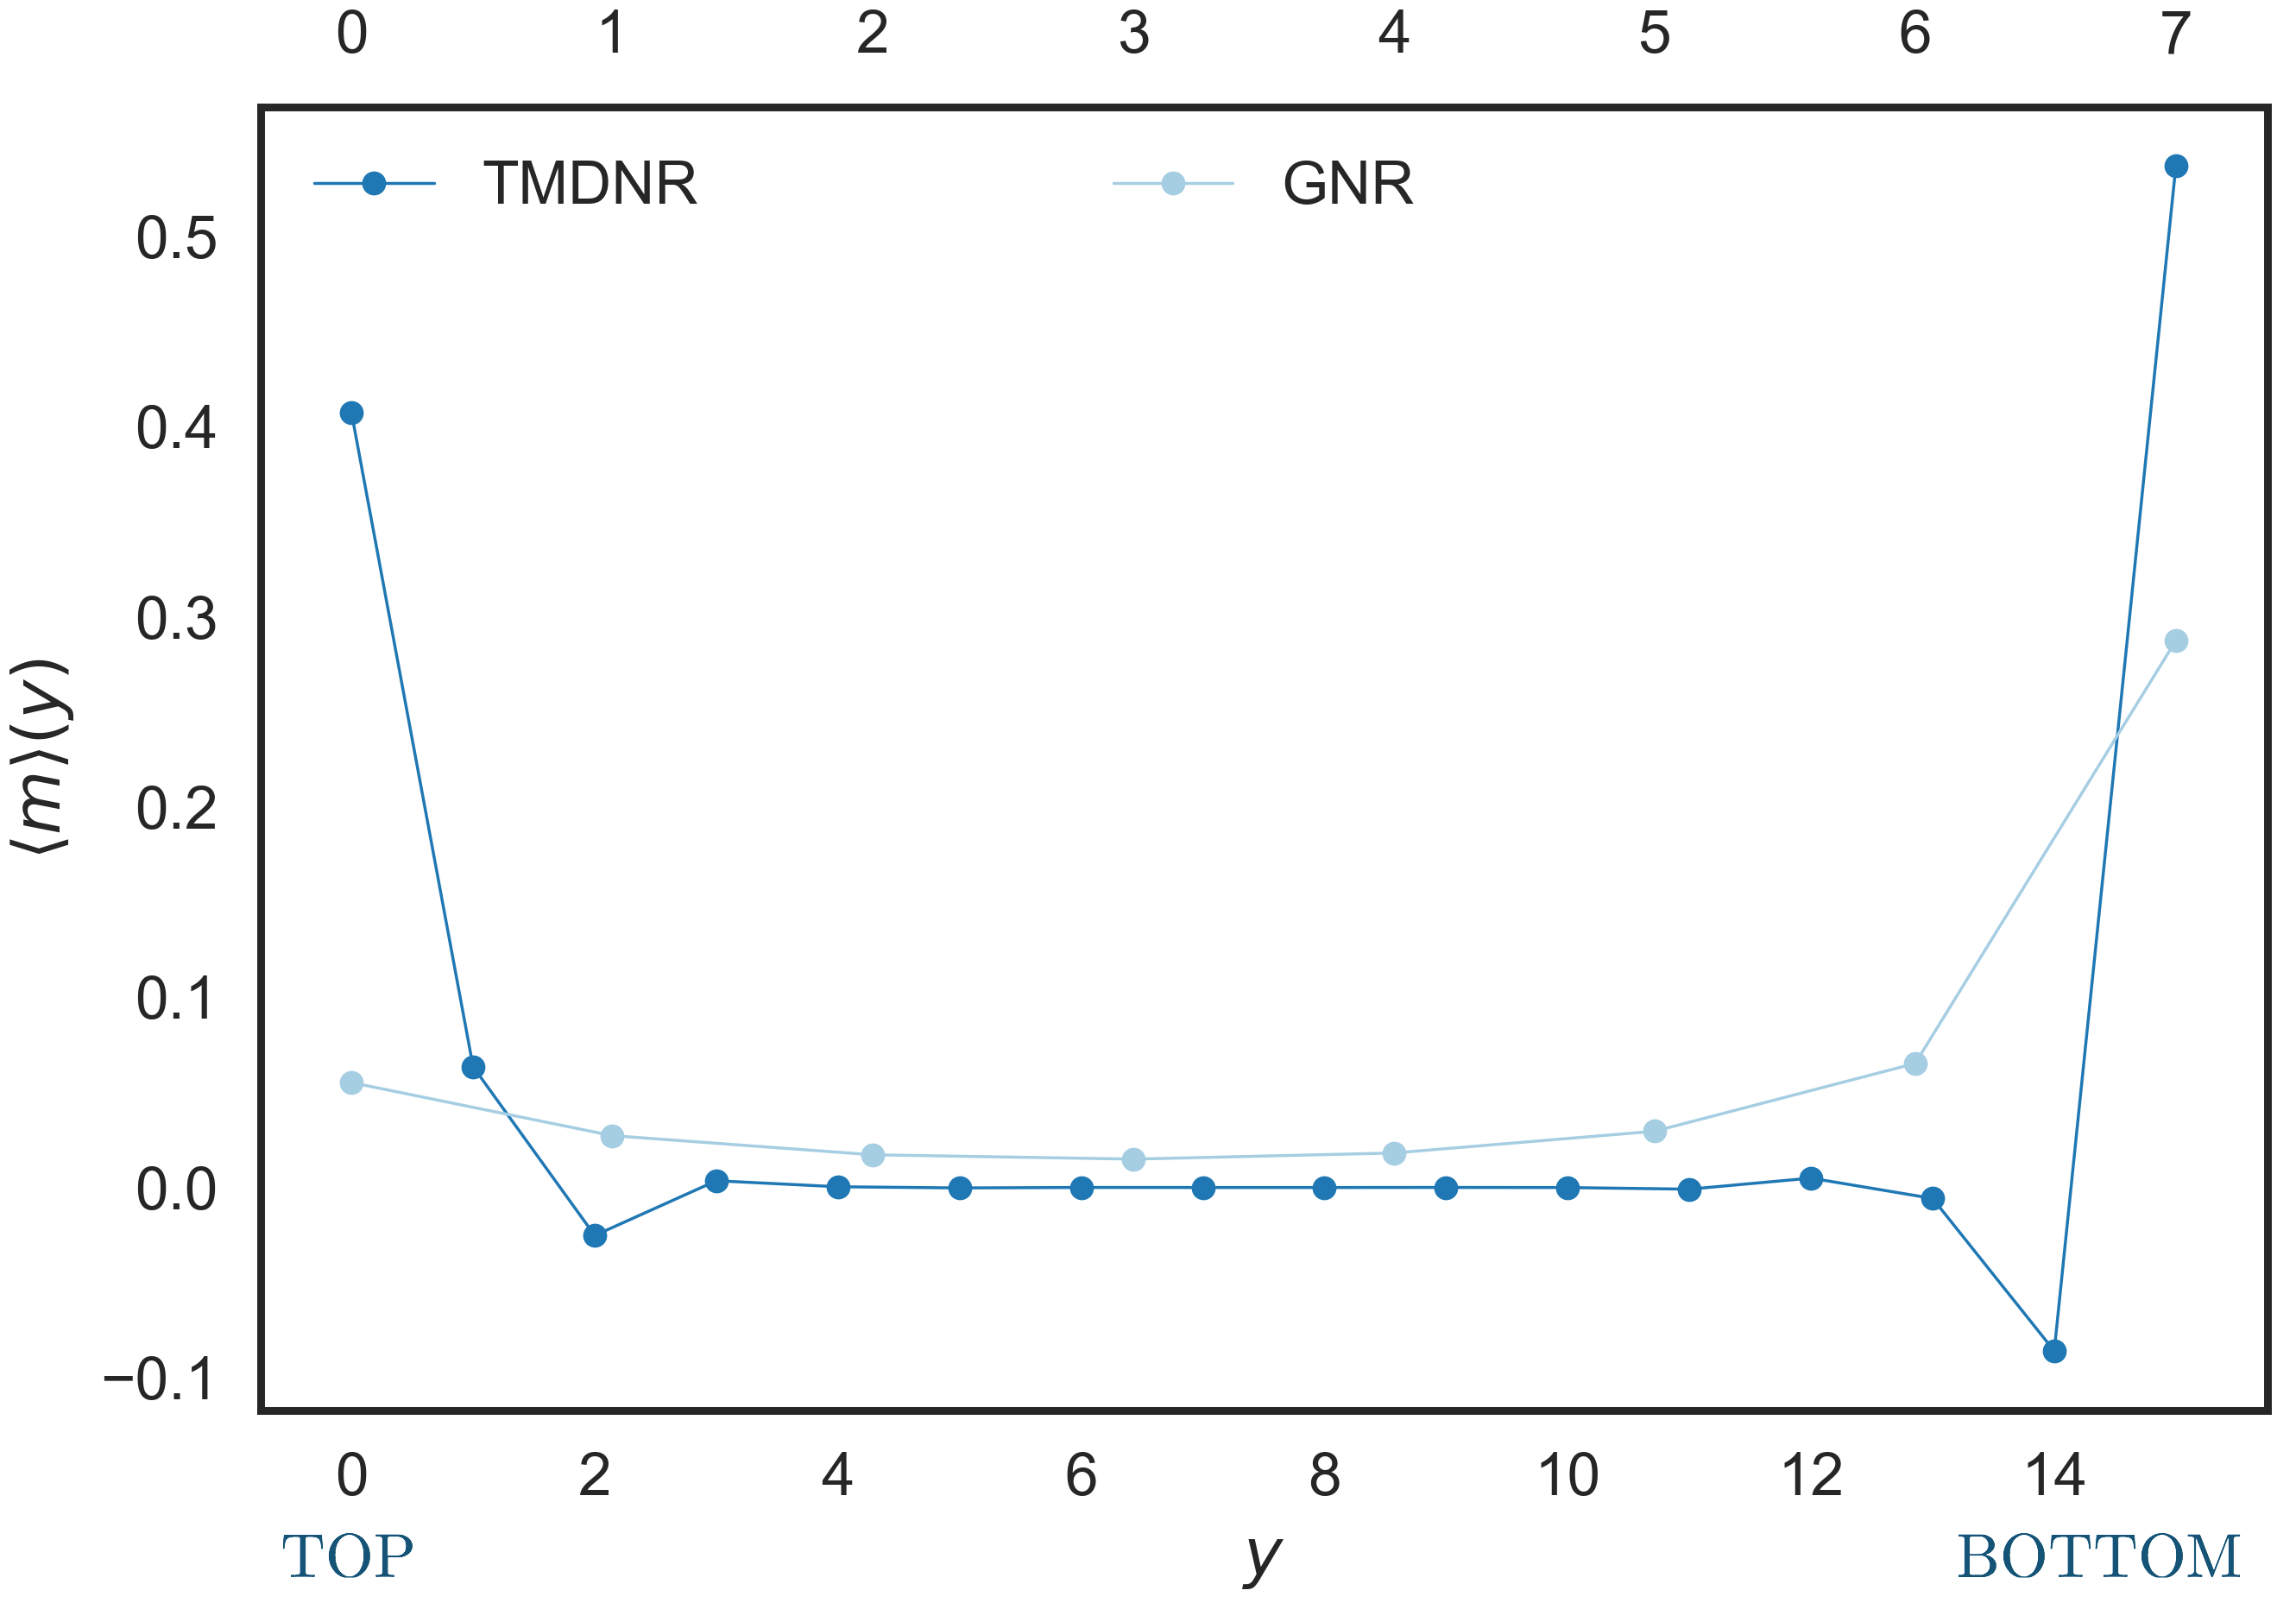
\includegraphics[scale=0.52]{Applications/magProf.png}
\hspace{0.9cm}
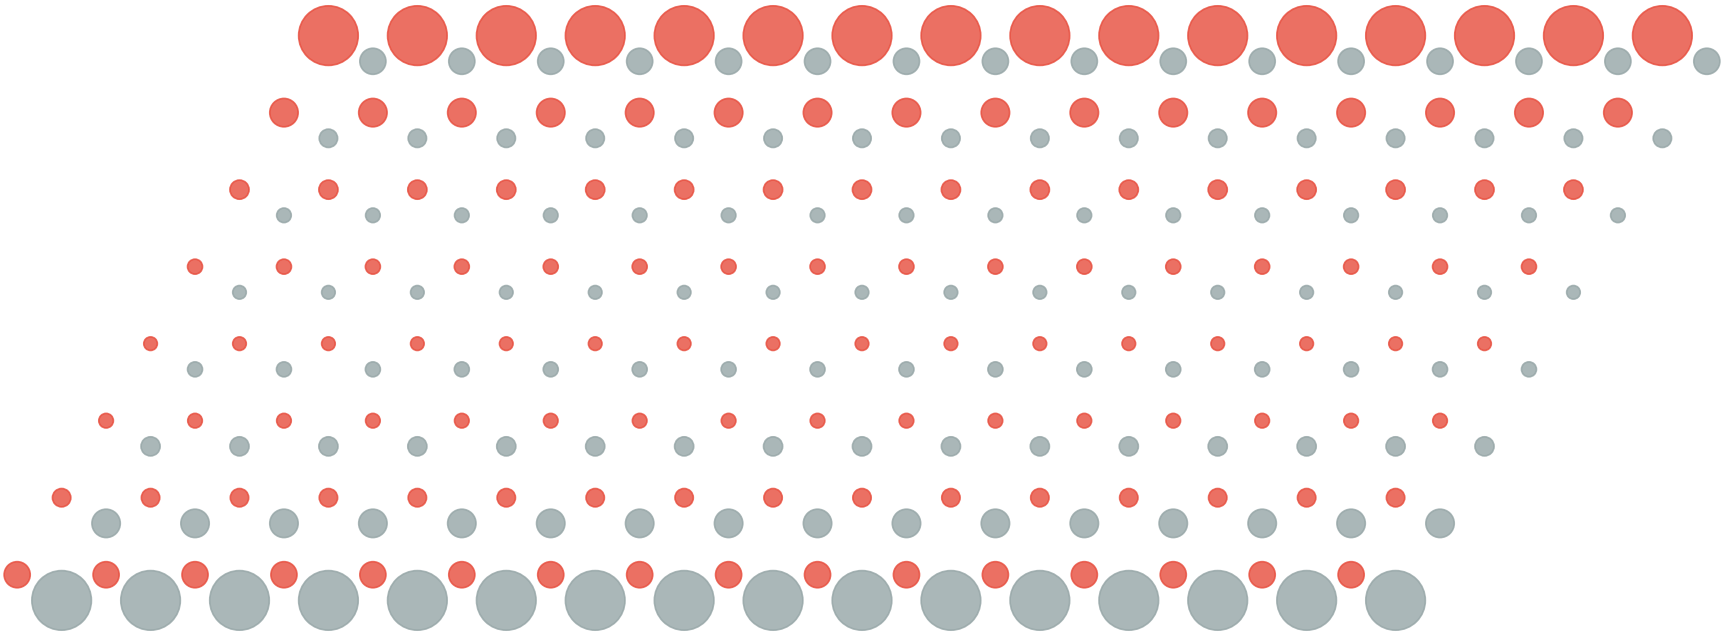
\includegraphics[scale=1.]{Applications/MFnanoribbon.png}
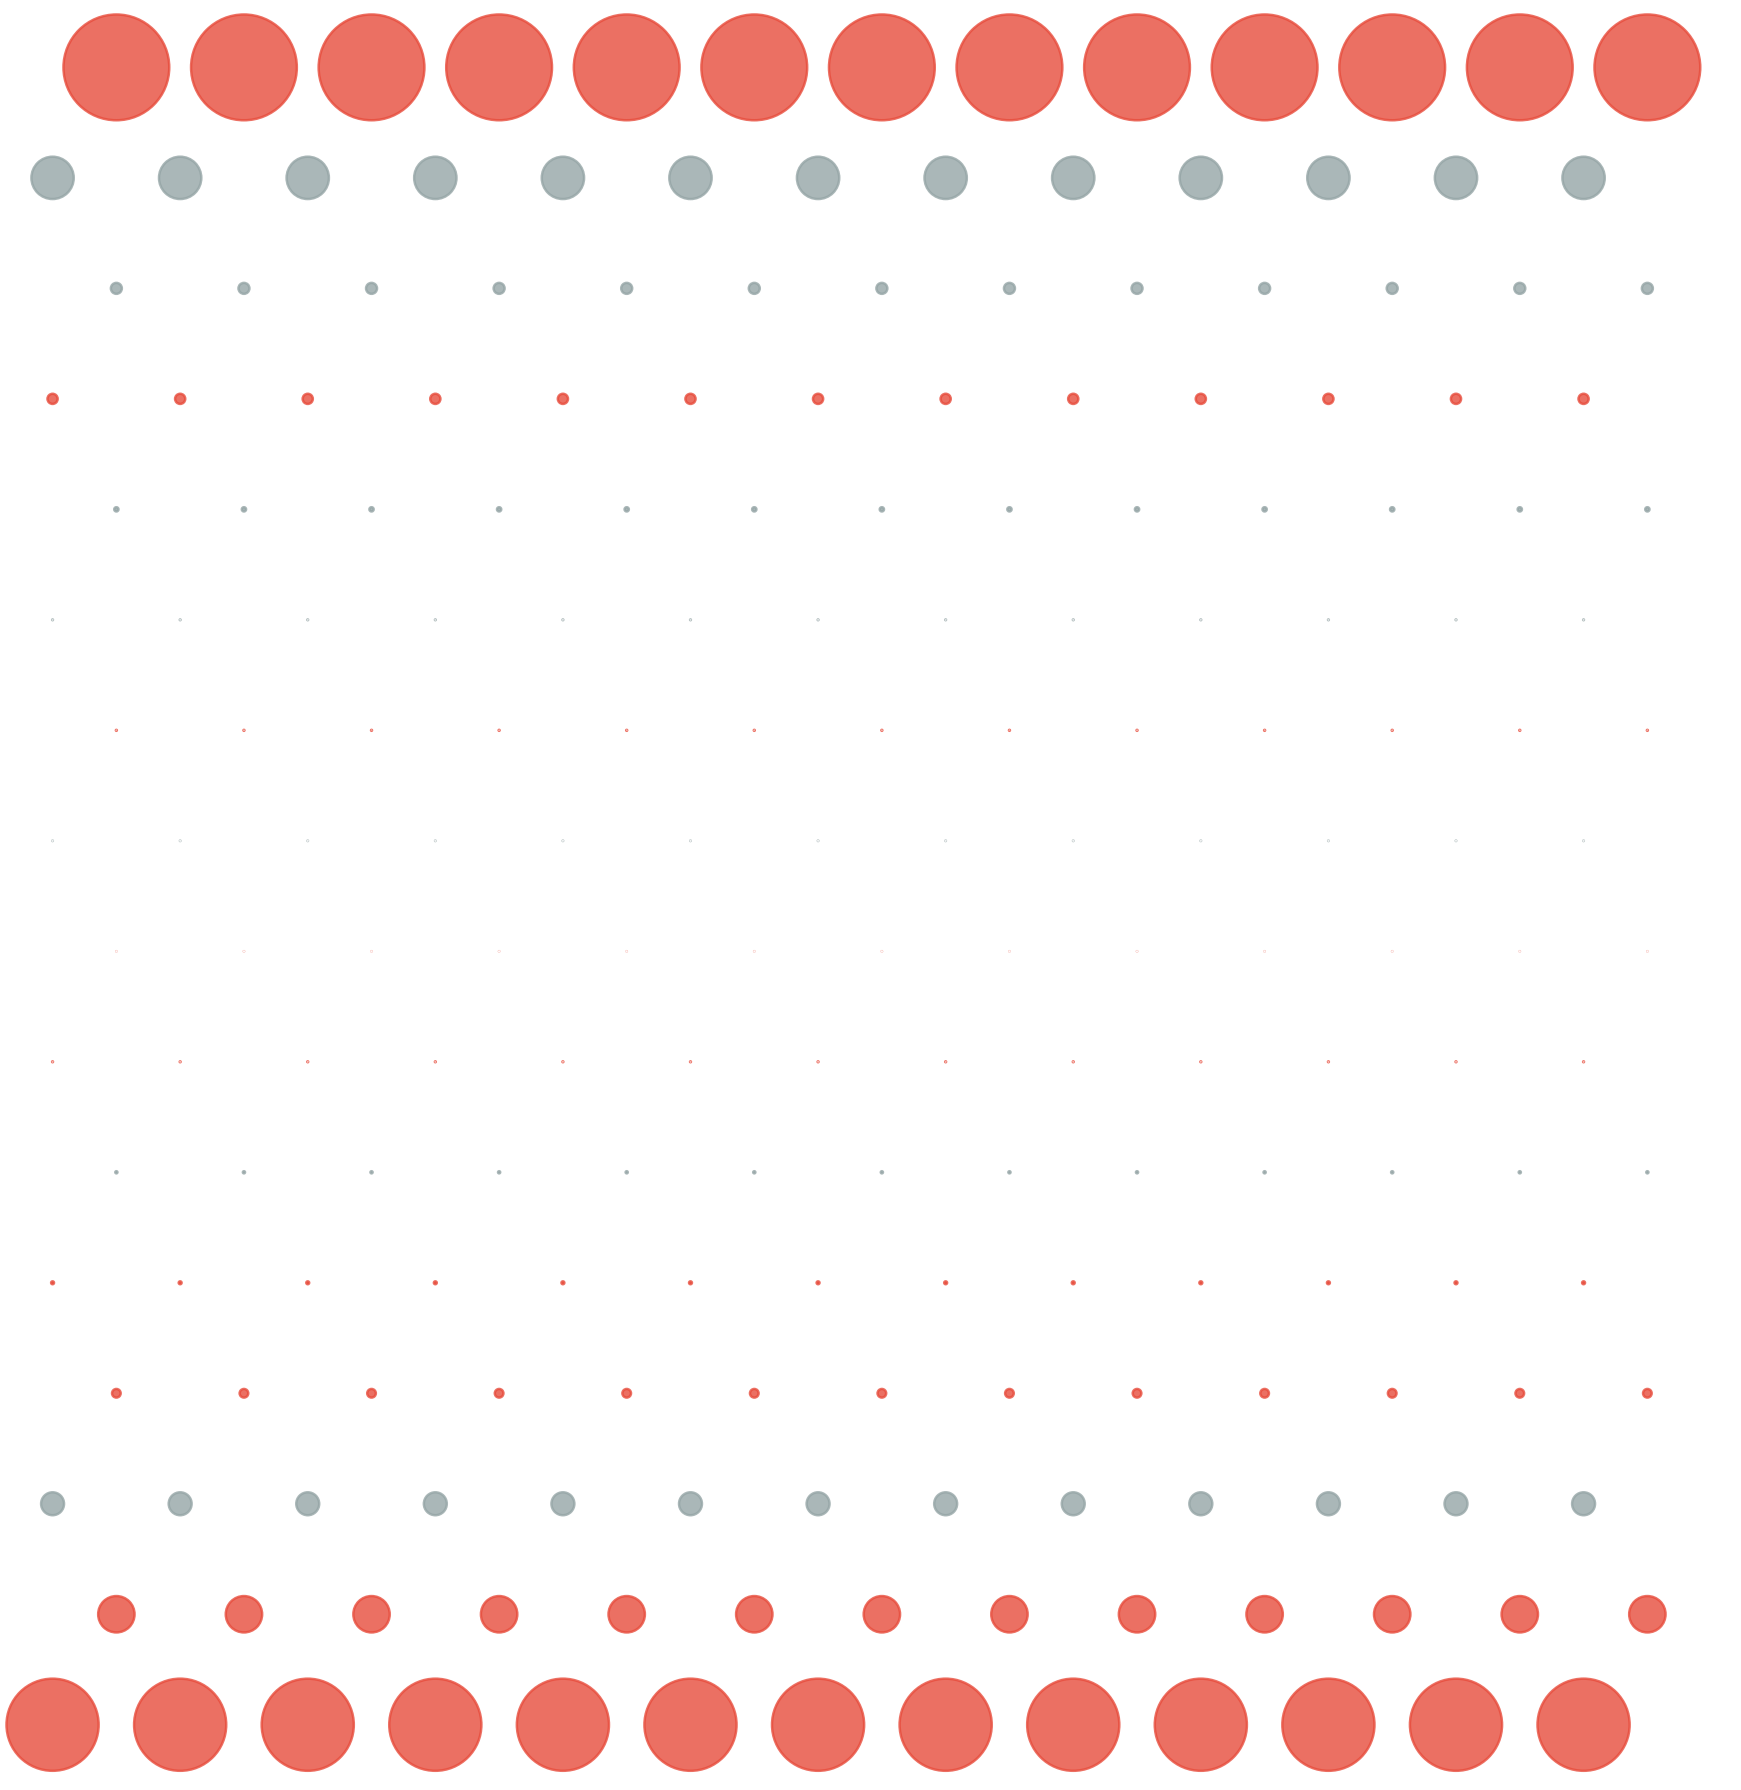
\includegraphics[scale=1.45]{Applications/lattice_Nx=512_Ny=16_U=20_beta=100.png}
	\caption[Comparison between the zero temperature MF solutions of the Hubbard model for a graphene nanoribbon(GNR) and a \acs{TMDNR}]{Comparison between the zero temperature MF solutions of the Hubbard model at half filling ($\left\langle n \right\rangle = 1$) for a $16 \times 8$ graphene nanoribbon (GNR) at $U=1.2t$ (left) and a \acs{TMDNR} with $N_y = 16$ at $U = 20| t_0 |$, and electron density $\left\langle n \right\rangle = 0.66$, the filling that corresponds to charge neutrality.Left: Comparison between the spin density profile along the ribbon's transverse direction $\left\langle m \right\rangle (y)$ (the obtained solution is constant along $x$) for the GNR and the \acs{TMDNR}.
Right: Ordered phases obtained in mean field for graphene and \ac{TMD} nanoribbons. 
The size of the dots corresponds to the magnitude of the spin, and red stands for a positive spin, while blue stands for a negative spin.}
	\label{fig:nanoGraphVsTMD}
\end{figure}
From now on, we take a \acs{TMDNR} with $N_y = 16$, $U = 20| t_0 |$ and $\left\langle n \right\rangle = 0.66$.
By solving the self-consistent equation iteratively, at zero temperature, for varying $U$, we find two phase transitions, with respective critical on-site interactions $U_{c_1} \approx 11.8 |t_0|$, and $U_{c_2} \approx 15.395 |t_0|$.
\begin{figure}[H]
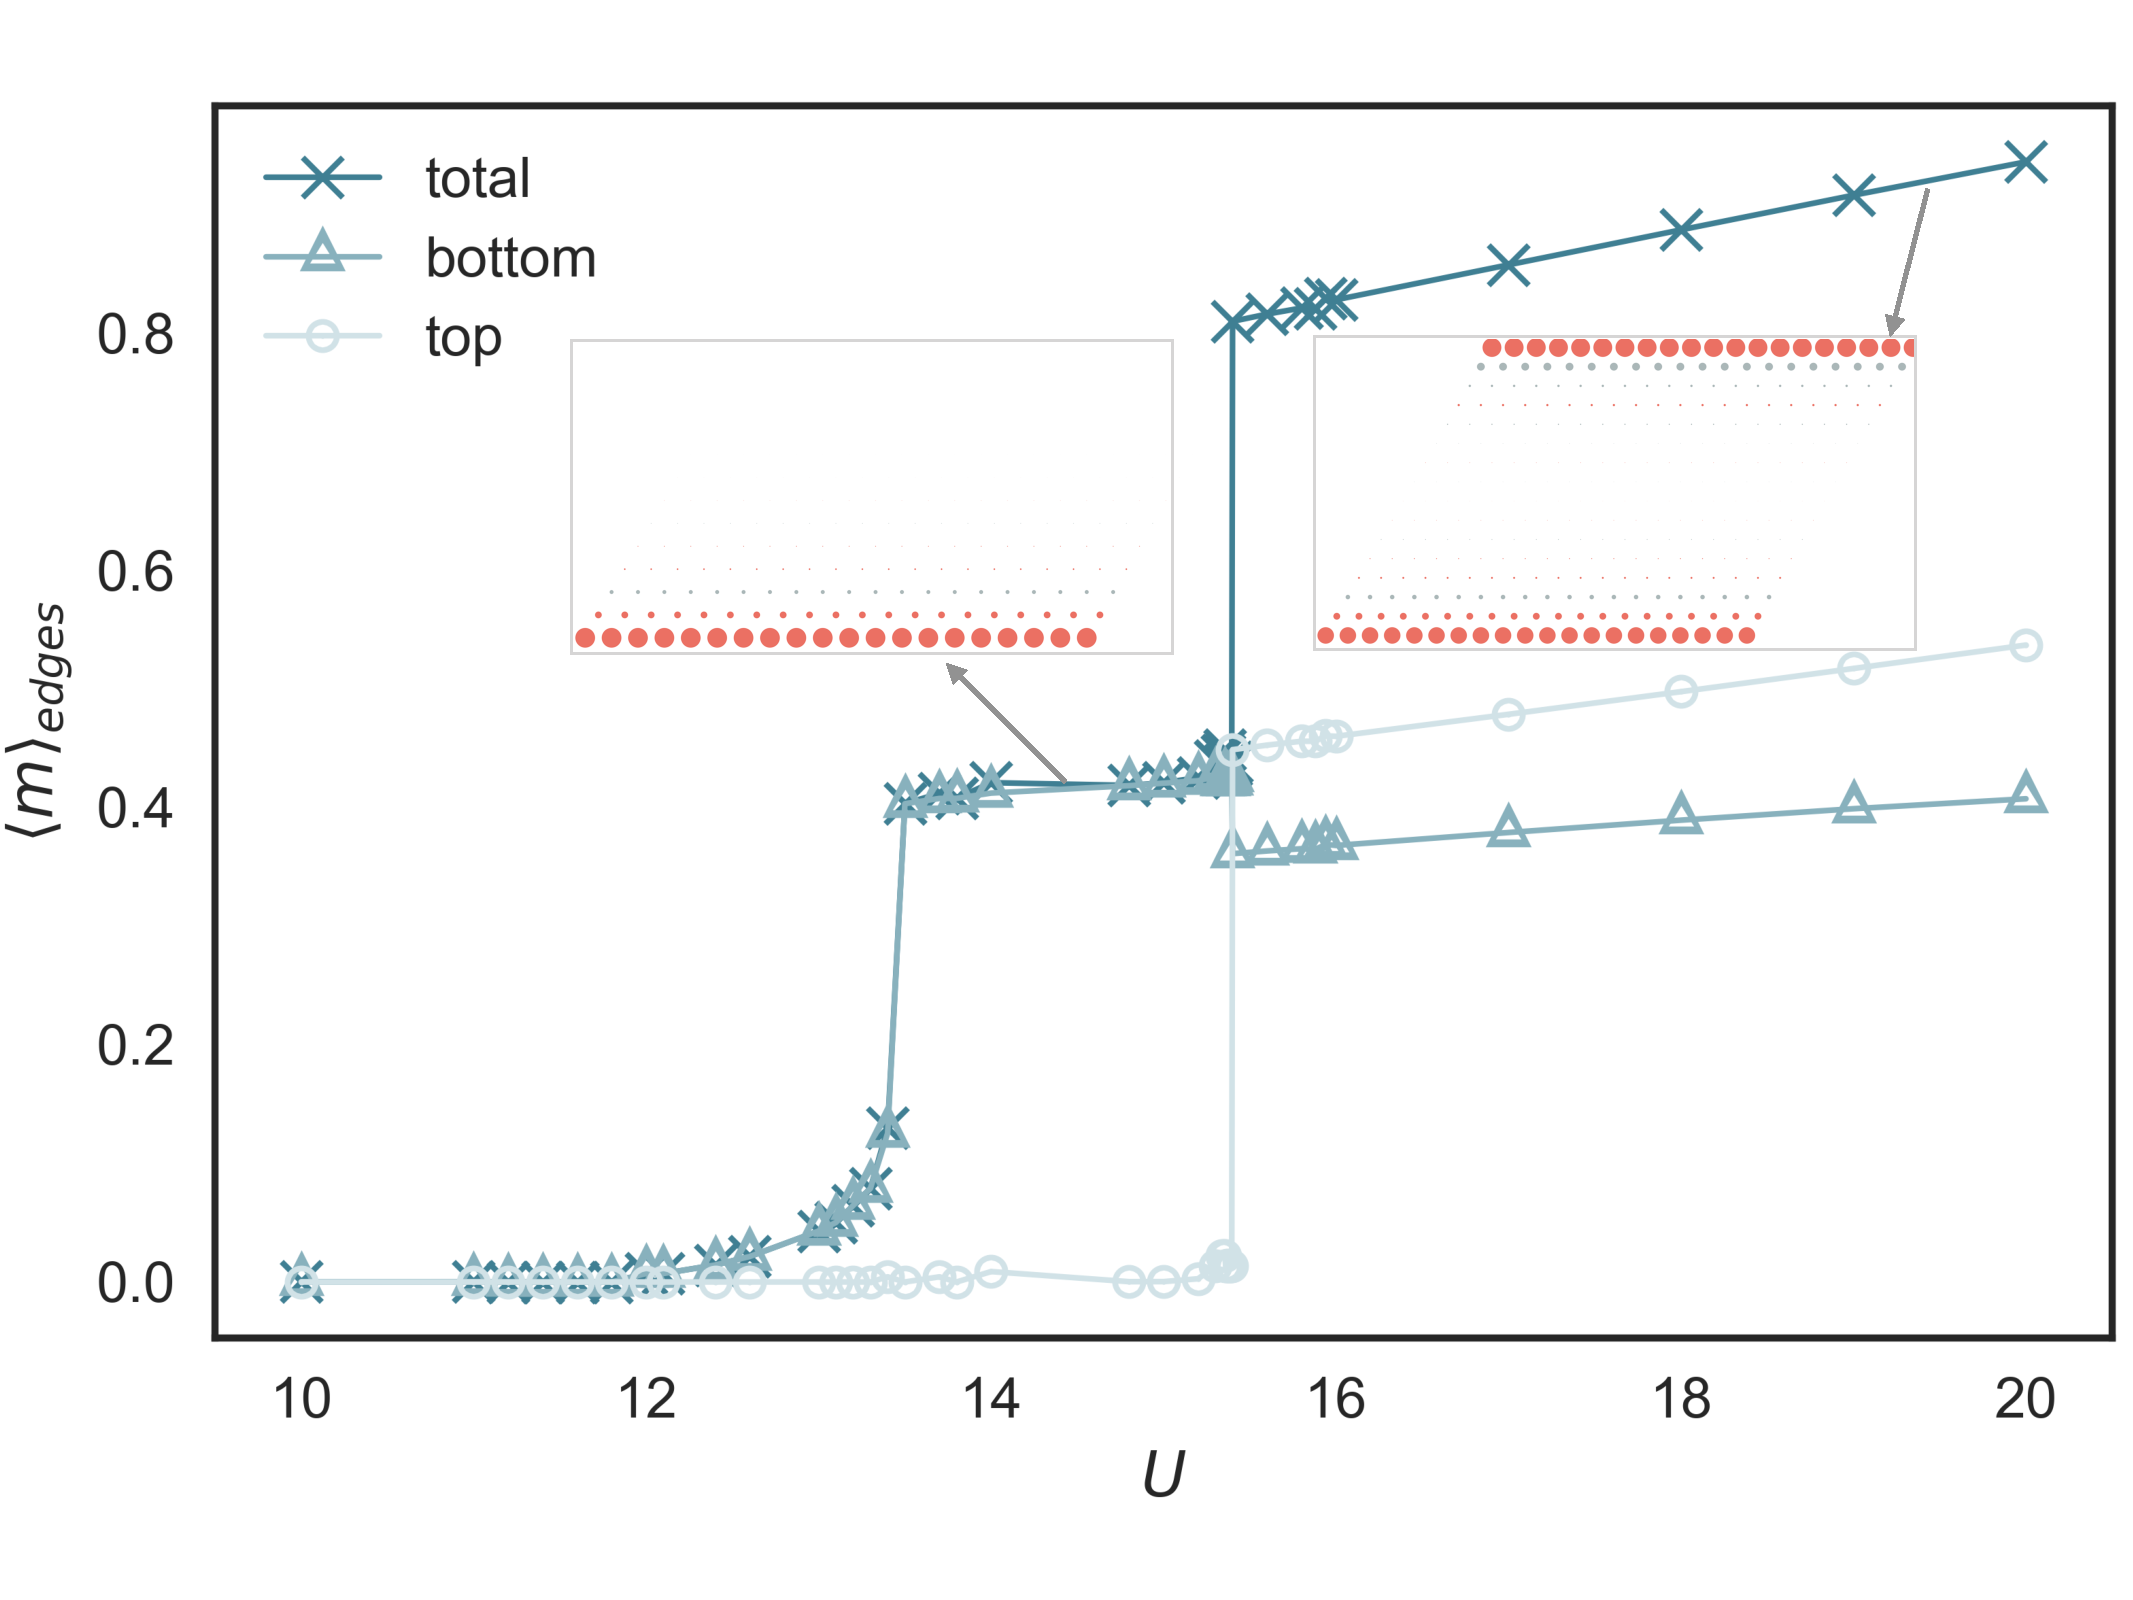
\includegraphics[trim={0cm 1.7cm 0cm 1.7cm},clip, scale =0.21]{Applications/tmd-mf/edge-mag.pdf}
\hspace{0.5cm}
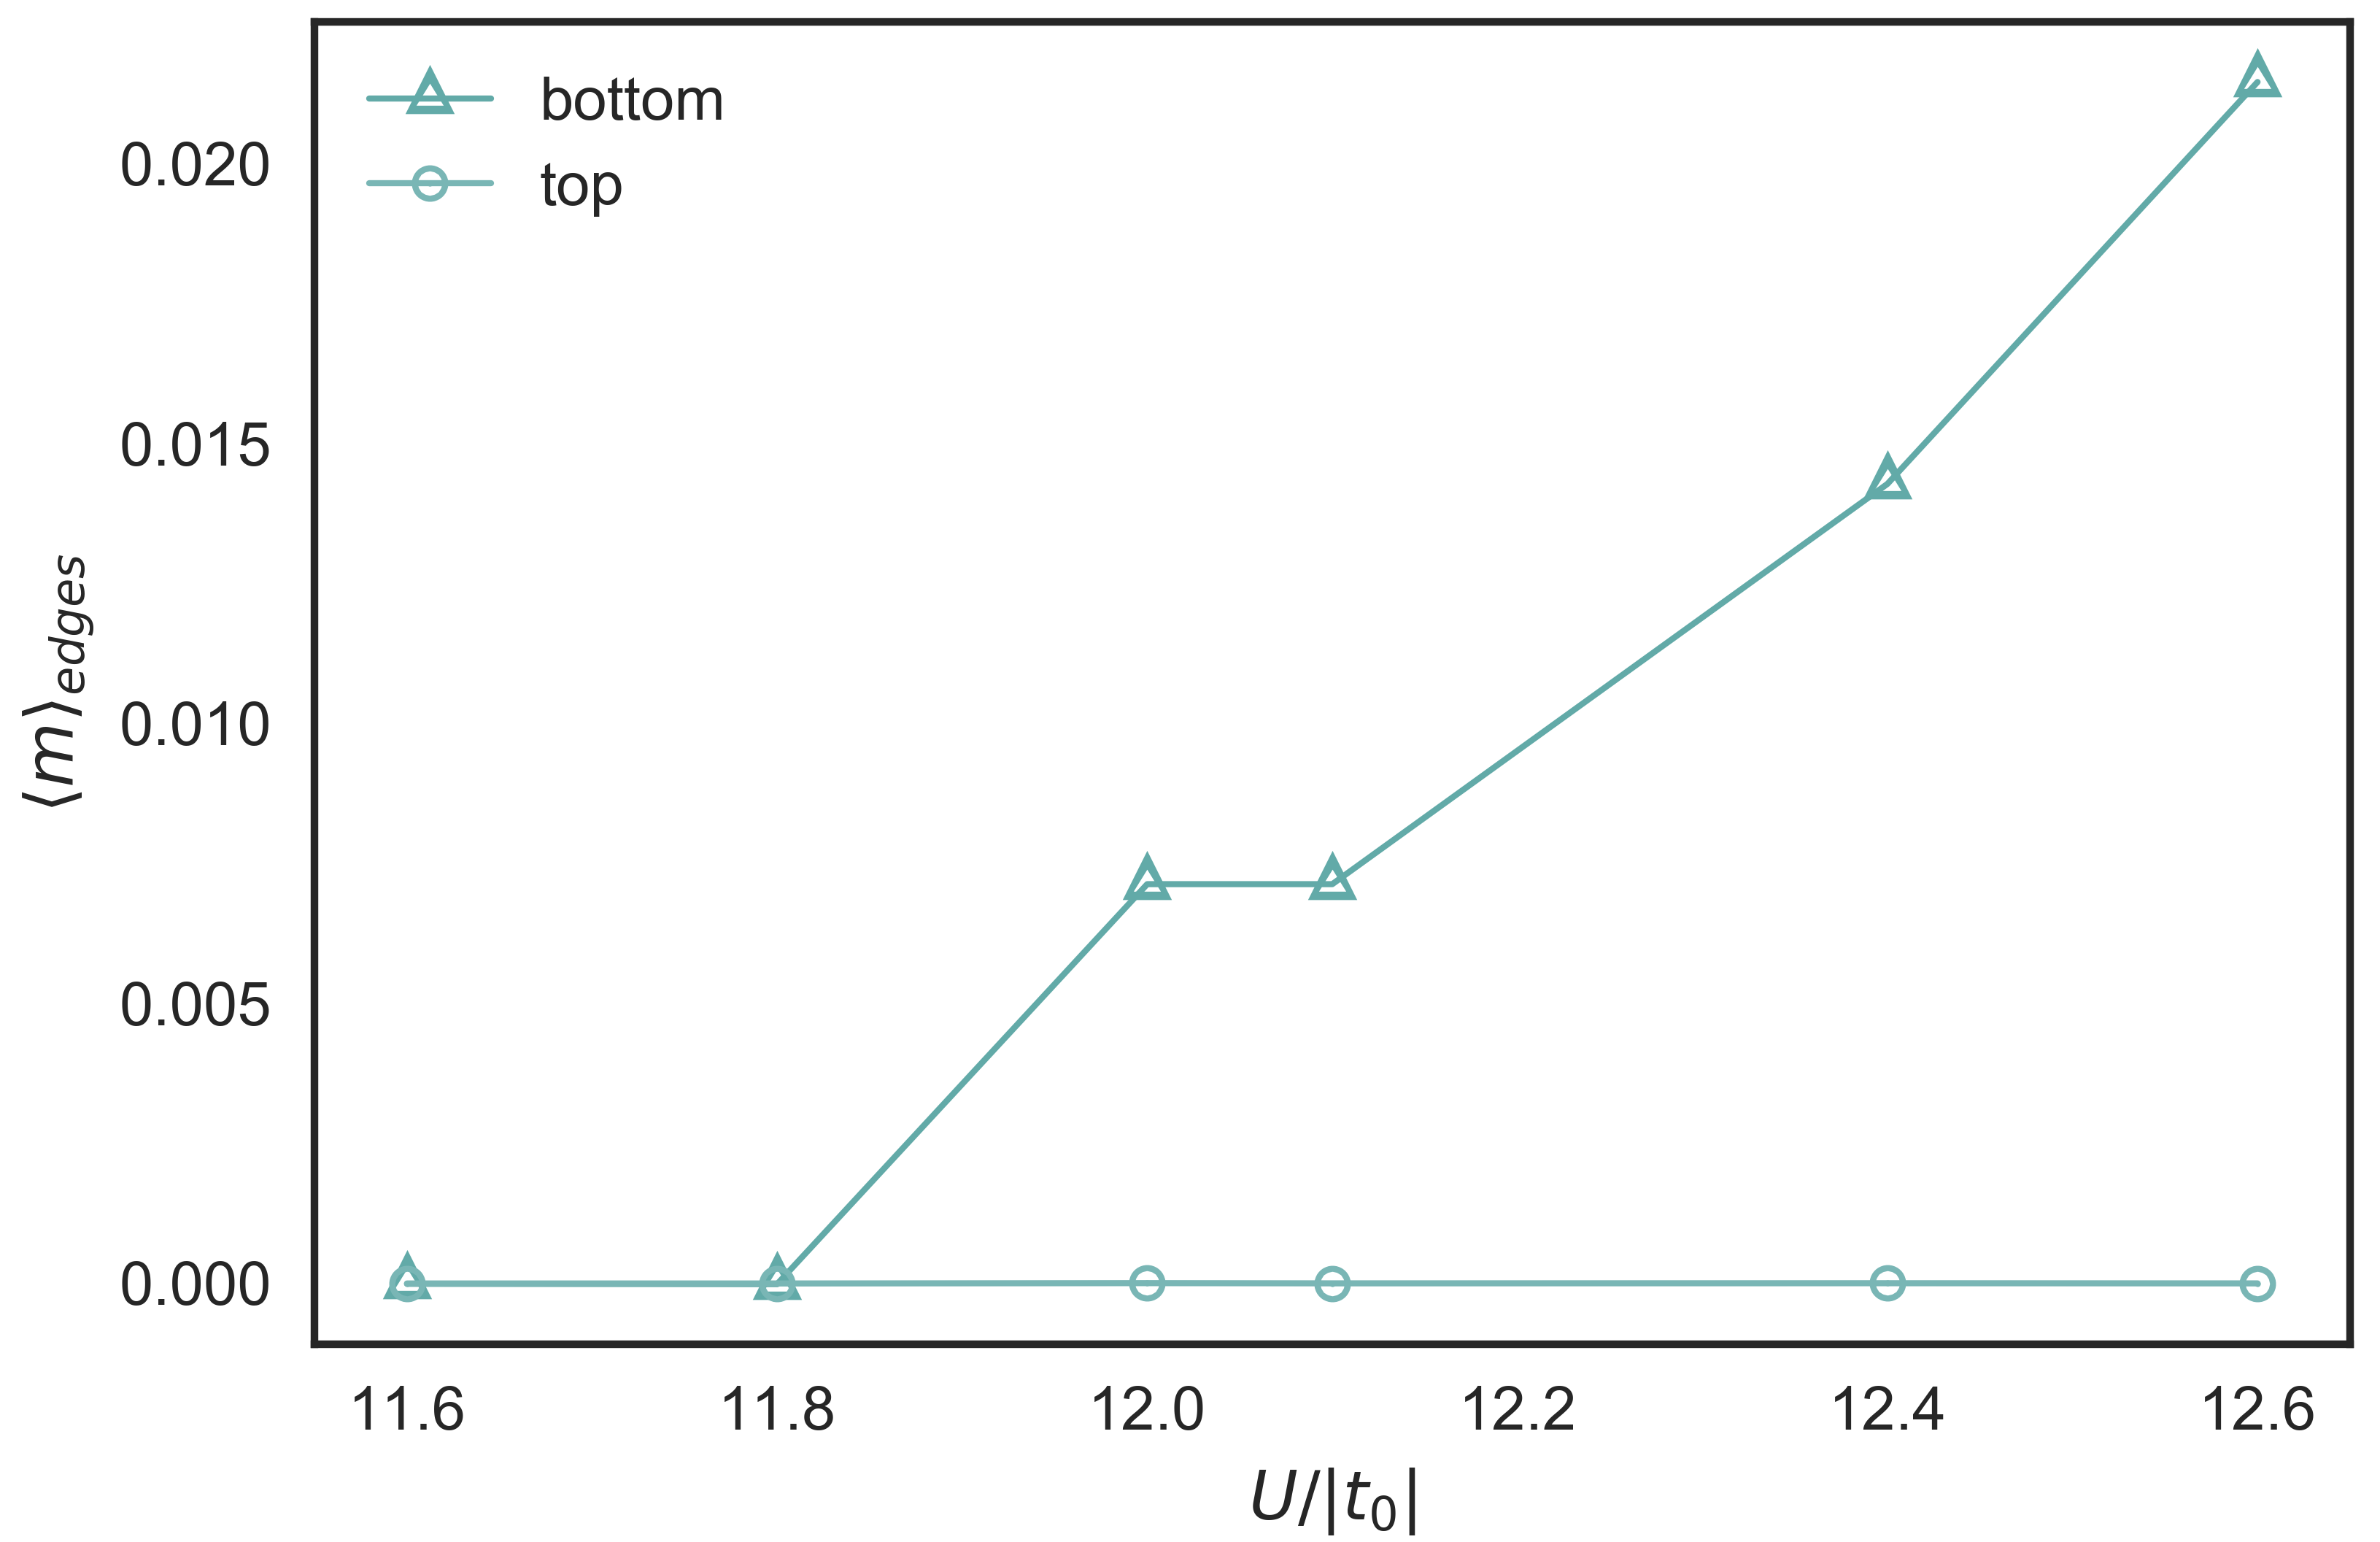
\includegraphics[scale=0.55]{Applications/tmd-mf/edge-magzoom1}
	\caption[Mean field phase diagram at zero temperature. Zoom-in of the first phase transition.]{Mean field phase diagram at zero temperature. Zoom-in of the first phase transition.
	\label{fig:zeroTphaseDiagram}}
\end{figure}
Compare the $y$-scales of Figs.(\ref{fig:zeroTphaseDiagram},\ref{fig:freeBands}).
One sees that the phase transition is much more abrupt in the latter than in the former, so that the first transition at $U_{c_1} \approx 11.8 |t_0|$ appears to be continuous, while the second one at $U_{c_2} \approx 15.395 |t_0|$ appears to be first order.
\begin{figure}[H]
\hspace{0.3cm}
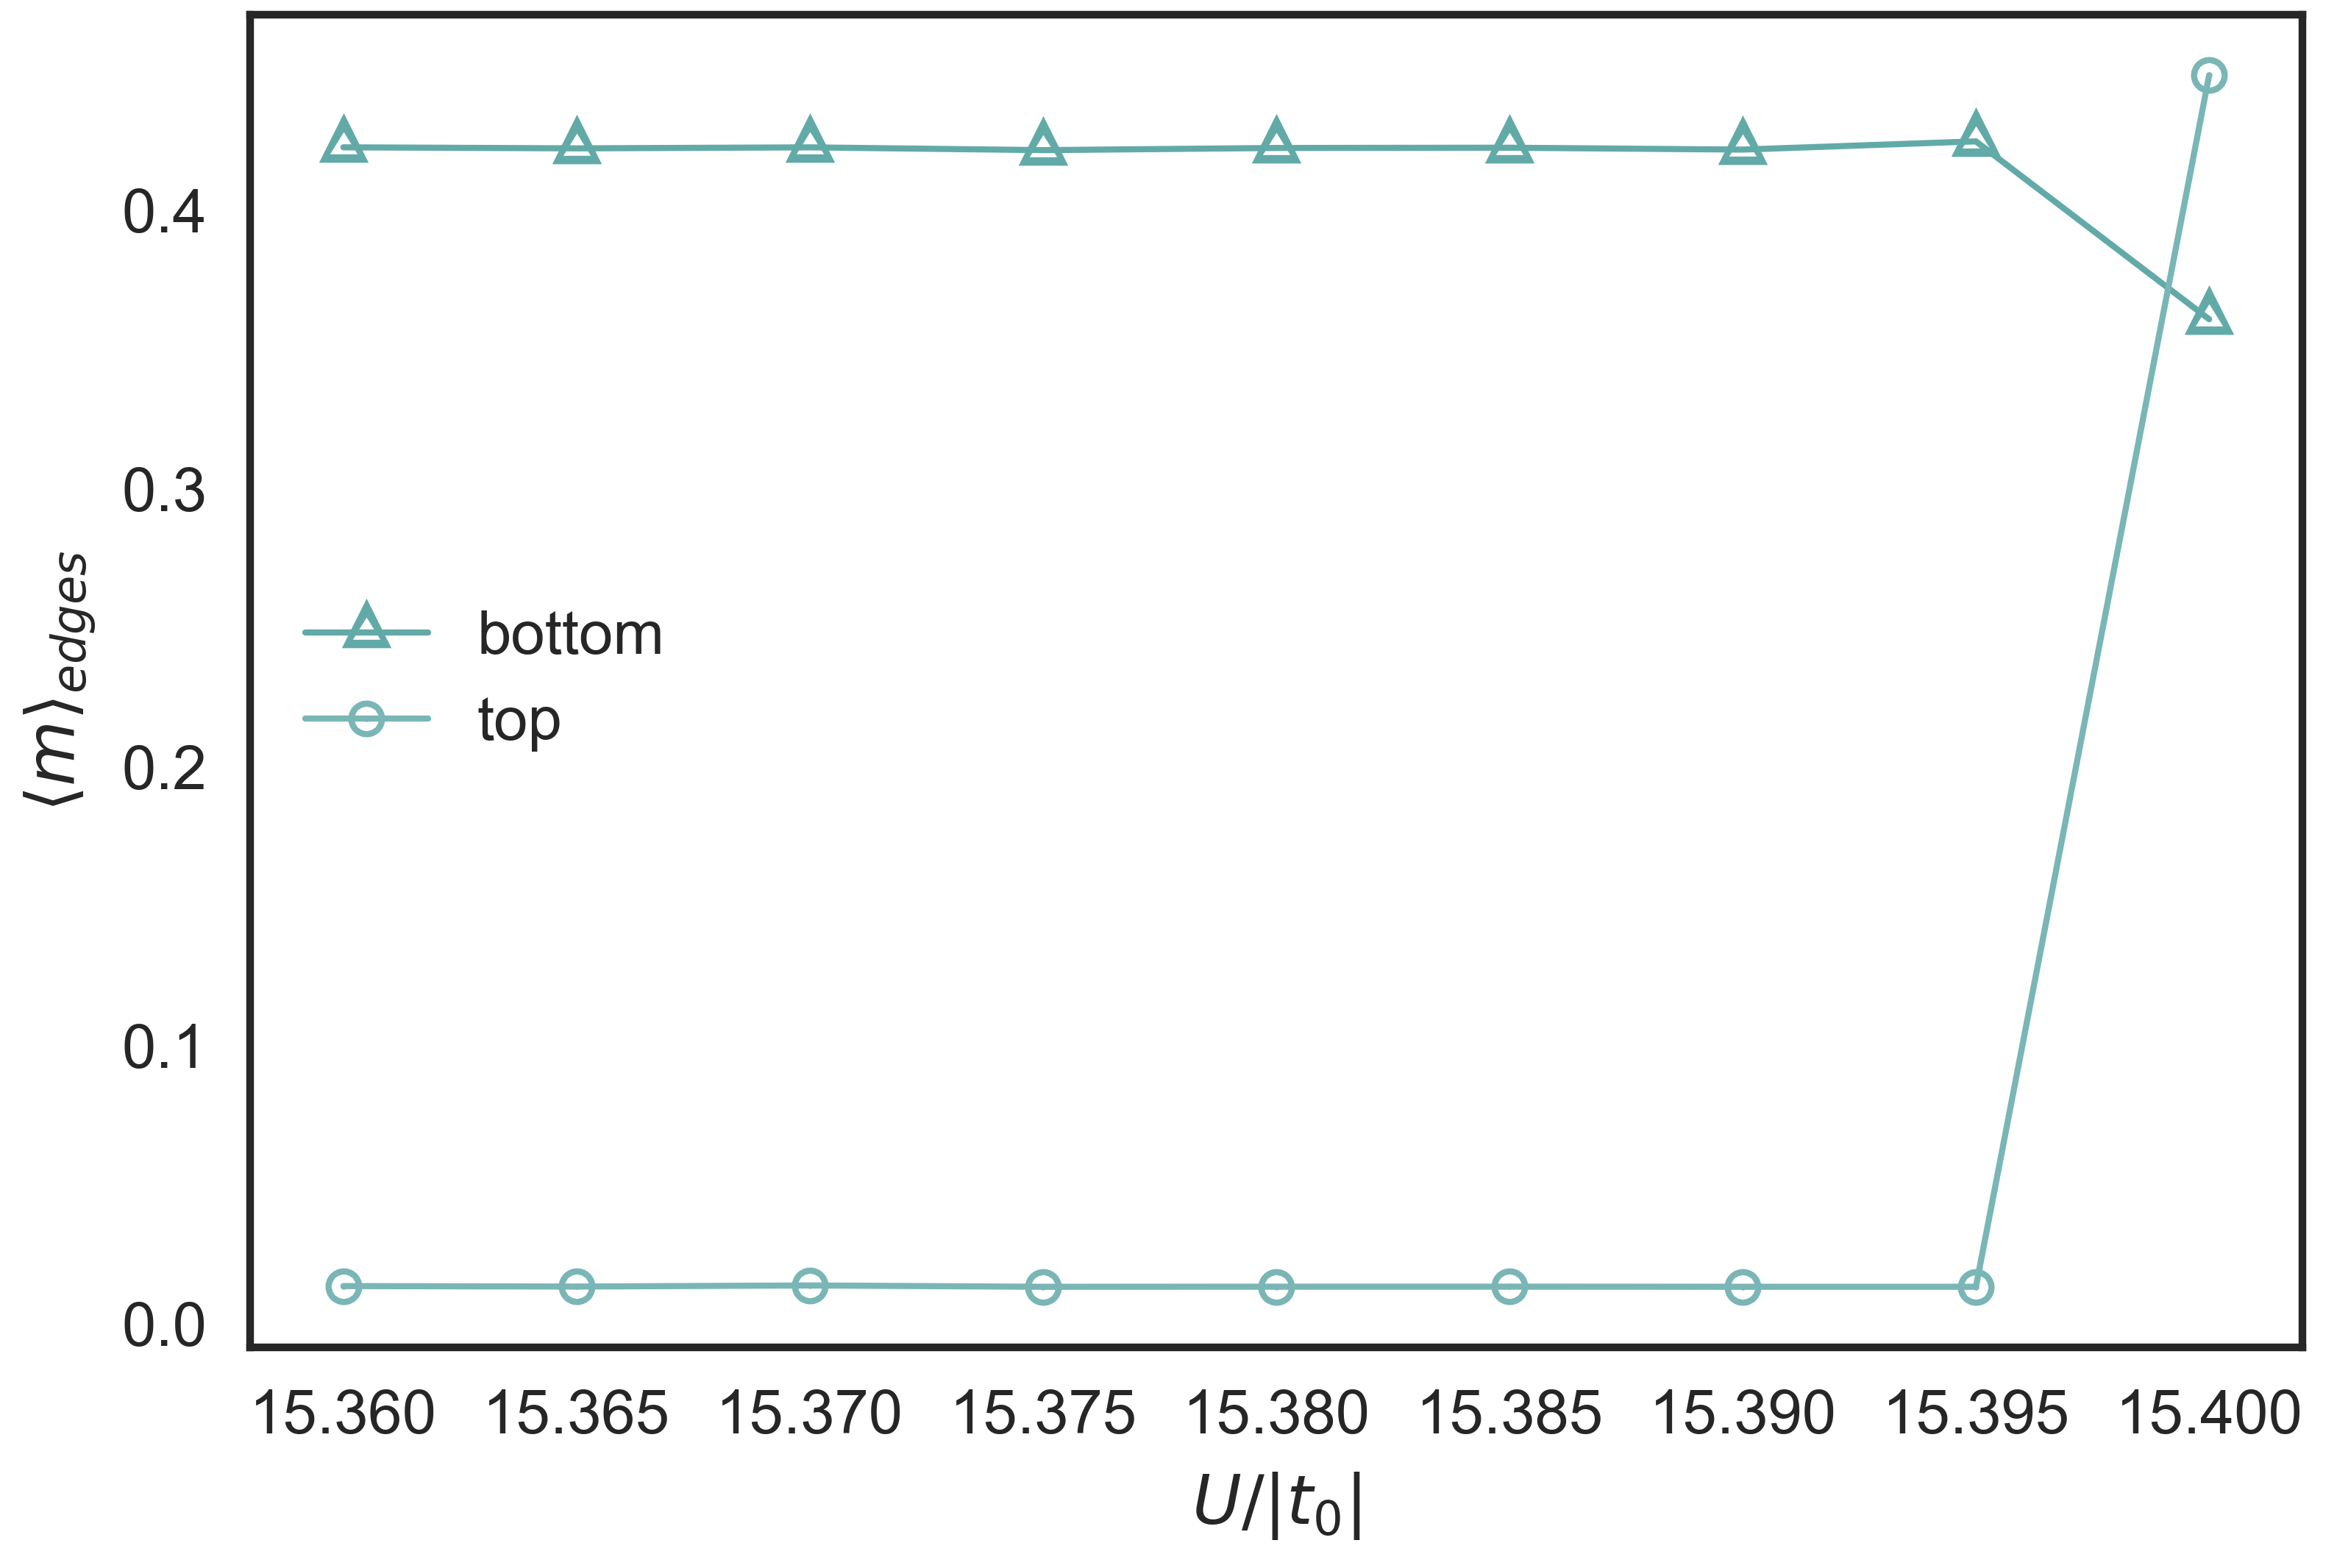
\includegraphics[scale=0.53]{Applications/tmd-mf/edge-magzoom2}
\hspace{0.5cm}
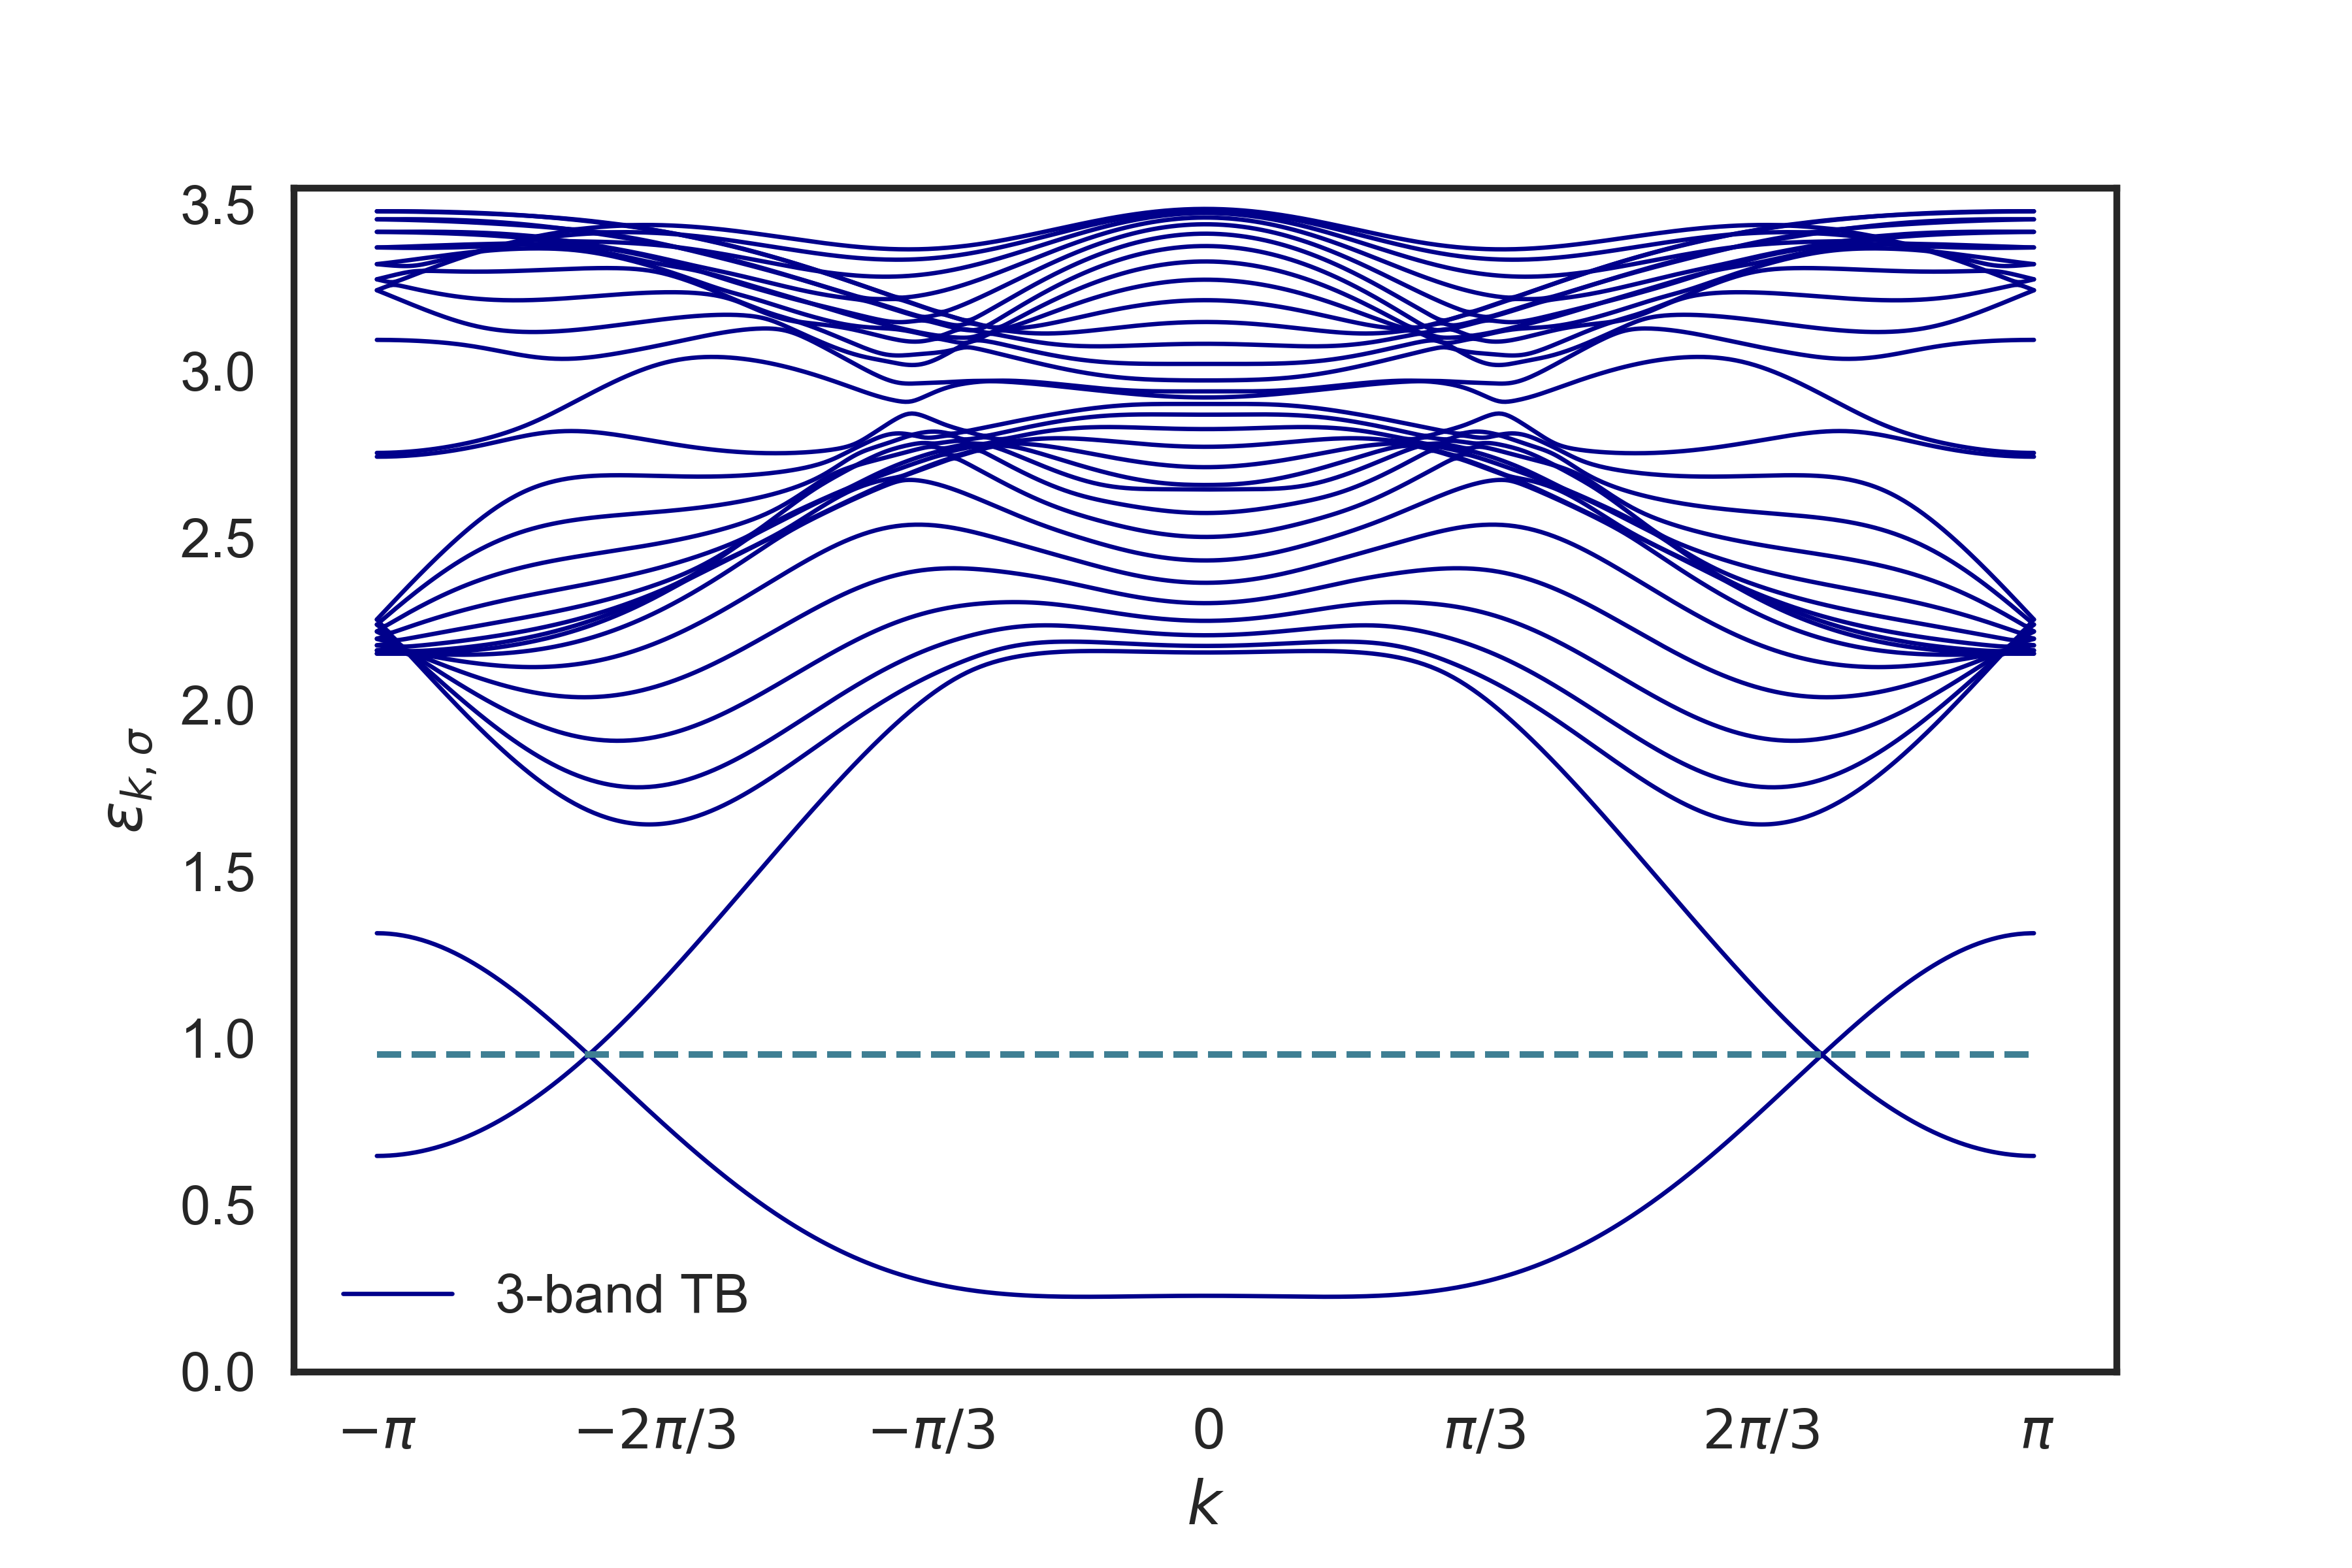
\includegraphics[scale=0.51]{Applications/tmd-mf/freeBands}
	\caption[Zoom-in of the second phase transition (as $U$ is increased). Band structure of the free-fermion problem.]{Left: Zoom-in of the second phase transition $U$ is increased. Right: Band structure of the free-fermion problem.
	\label{fig:freeBands}}
\end{figure}
To understand the effect of the on-site interaction at the mean field level, we start by comparing the band structure of the free problem to the mean field band structure, for $U$ well within the ordered phase.
\begin{figure}[H]
\centering
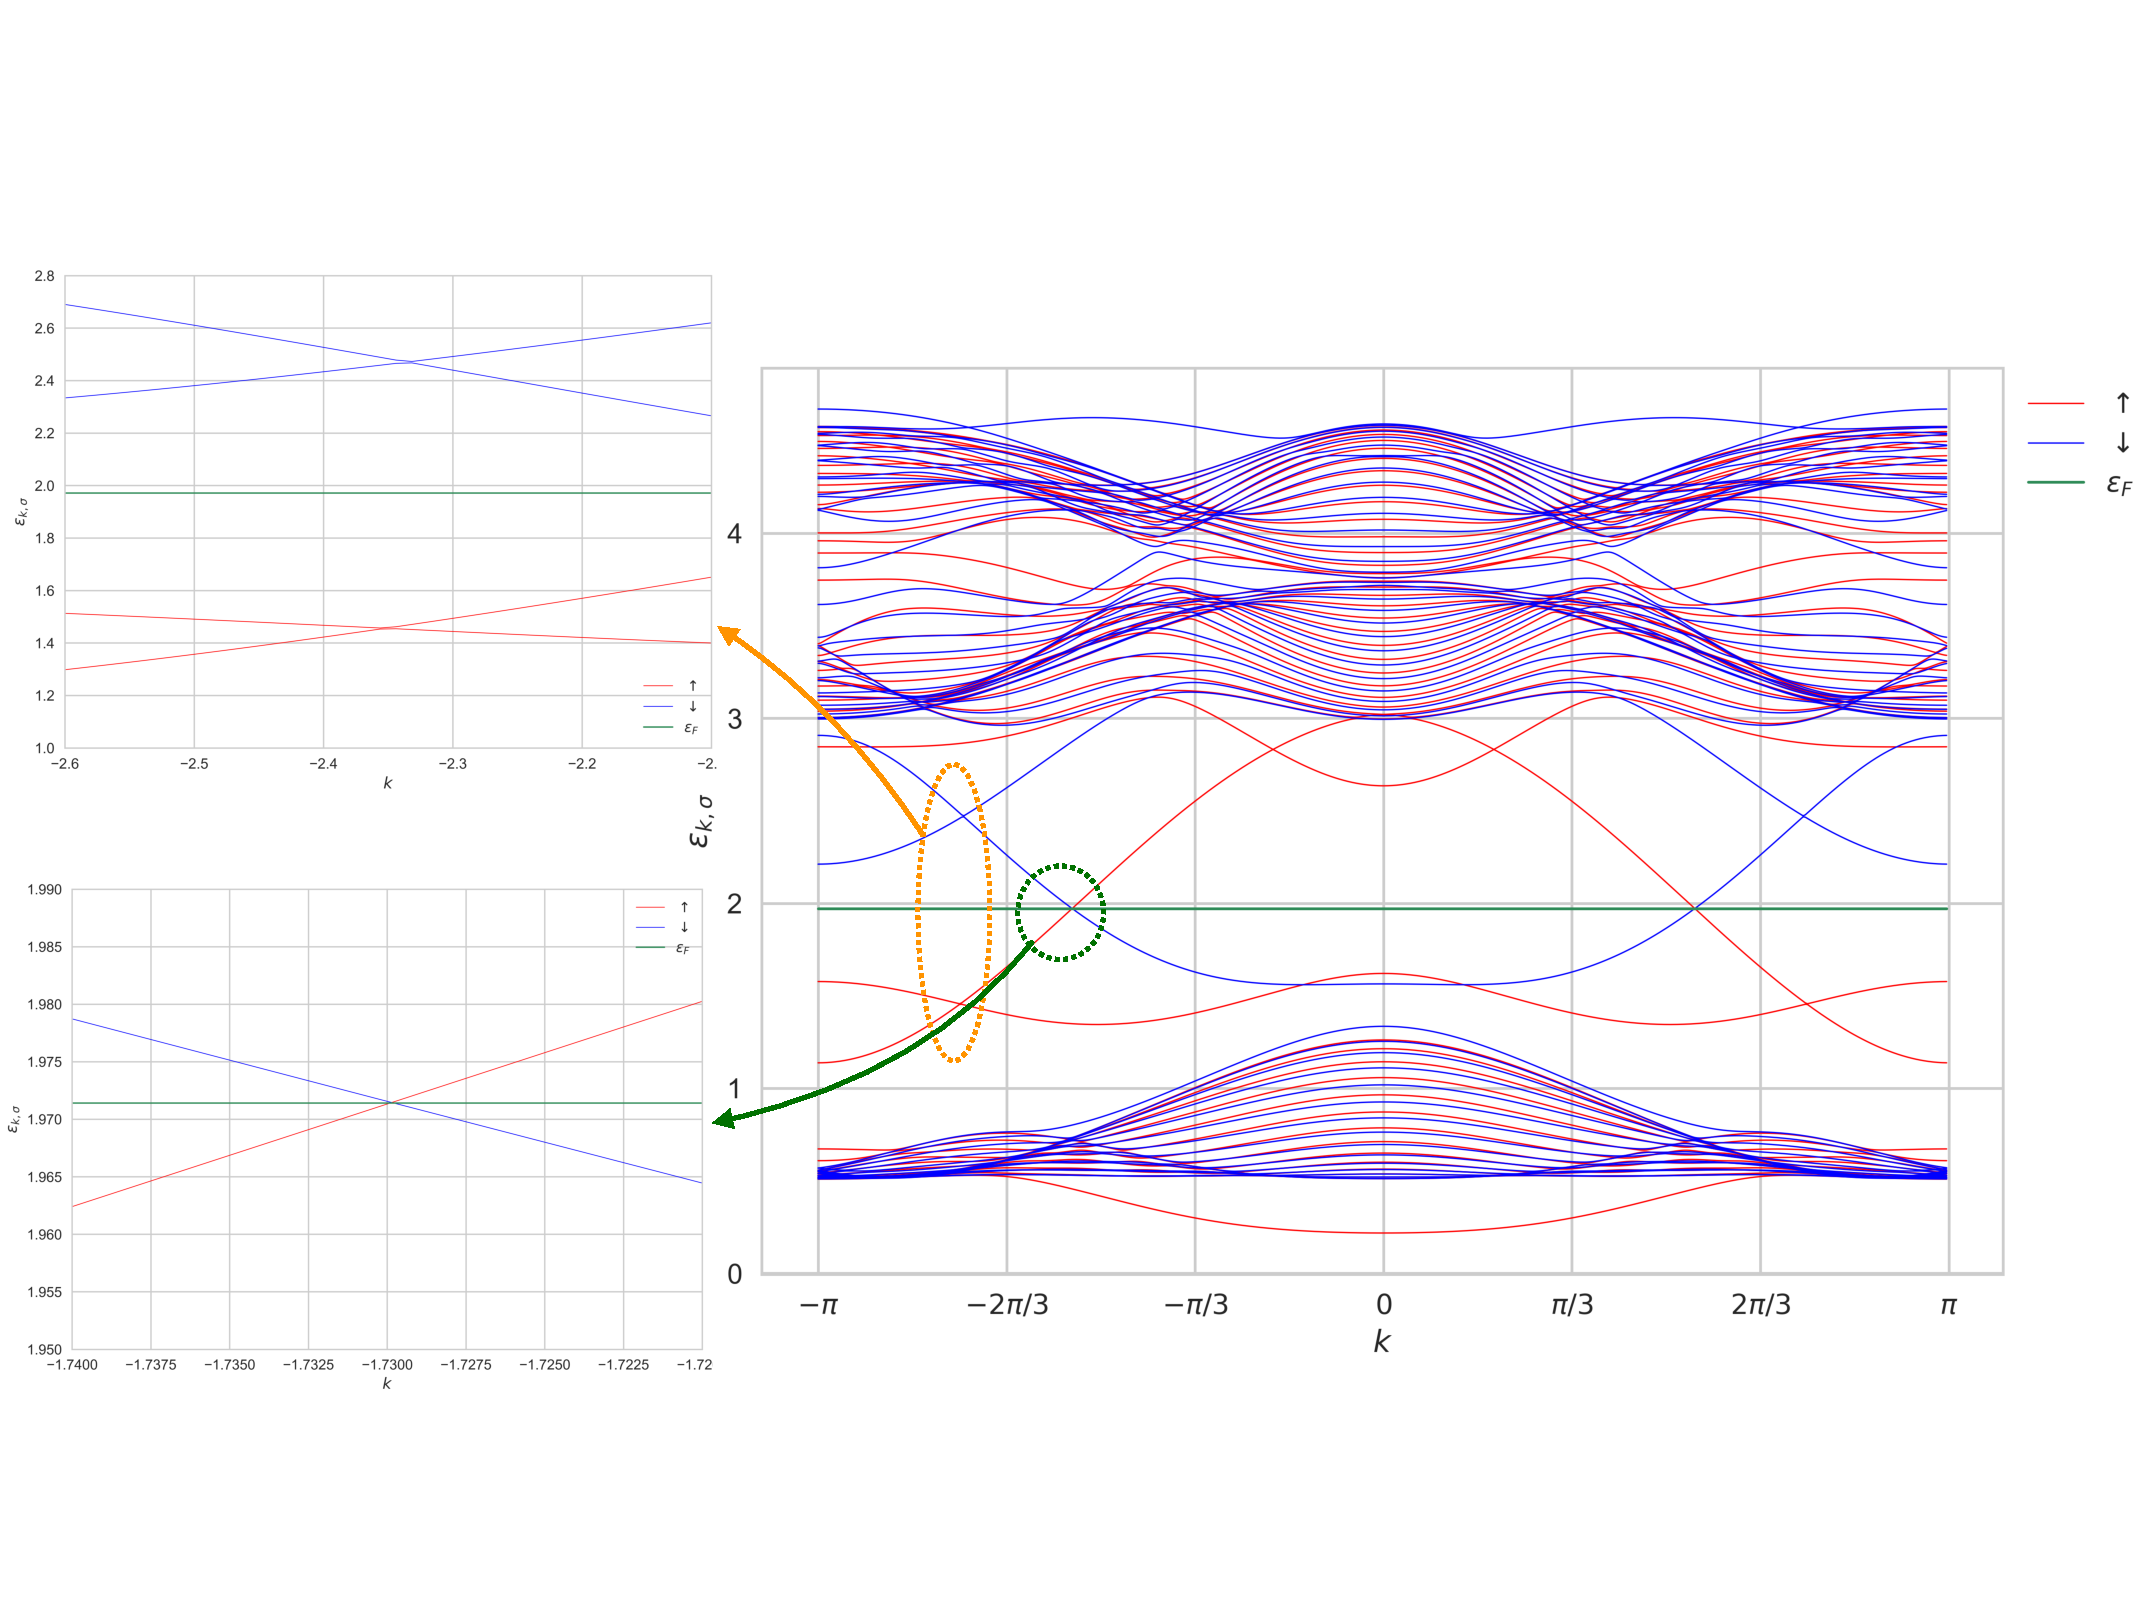
\includegraphics[trim={0cm 3cm 0cm 4cm},clip, scale =0.35]{Applications/tmd-mf/bandsZoomed.pdf}
	\caption[$T=0$ mean field band structure for a \ac{TMDNR} of width $N_y = 16$ in the ordered phase, at $U=20 | t_0 |$.]{$T=0$ mean field band structure for a \ac{TMDNR} of width $N_y = 16$ in the ordered phase ($U=20 | t_0 |$).}
	\label{fig:bandsZoomed}
\end{figure}

The first two aspects to notice are that spin degeneracy has been lifted, and that the shape of the bands has been distorted.
The part of the bands near the Fermi energy $\varepsilon_F$ determines the physics of the phase.
The interplay between the geometry of the tight-binding model, its parameters, the on-site interaction and temperature gives rise to different phases since it determines the shape of the bands and the location of the Fermi energy corresponding to charge neutrality.

In Fig.(\ref{fig:bandsZoomed}), two changes with respect to the free bands of Fig.(\ref{fig:freeBands}) are crucial:
the K-point splitting (circled in yellow), corresponding to a region where one of the bands stays below the Fermi energy, while the other stays above - this leads to spin polarization of the eigenstates associated with these energies; the band crossing (circled in green) - as $U$ varies, and the bands move upward or downward, and eventually distort, the states around this band crossing become either occupied or unoccupied, and since two opposite spin bands meet (\emph{at right angles}) at this point, this will most likely lead to spin polarized states.

\begin{figure}[H]
\centering
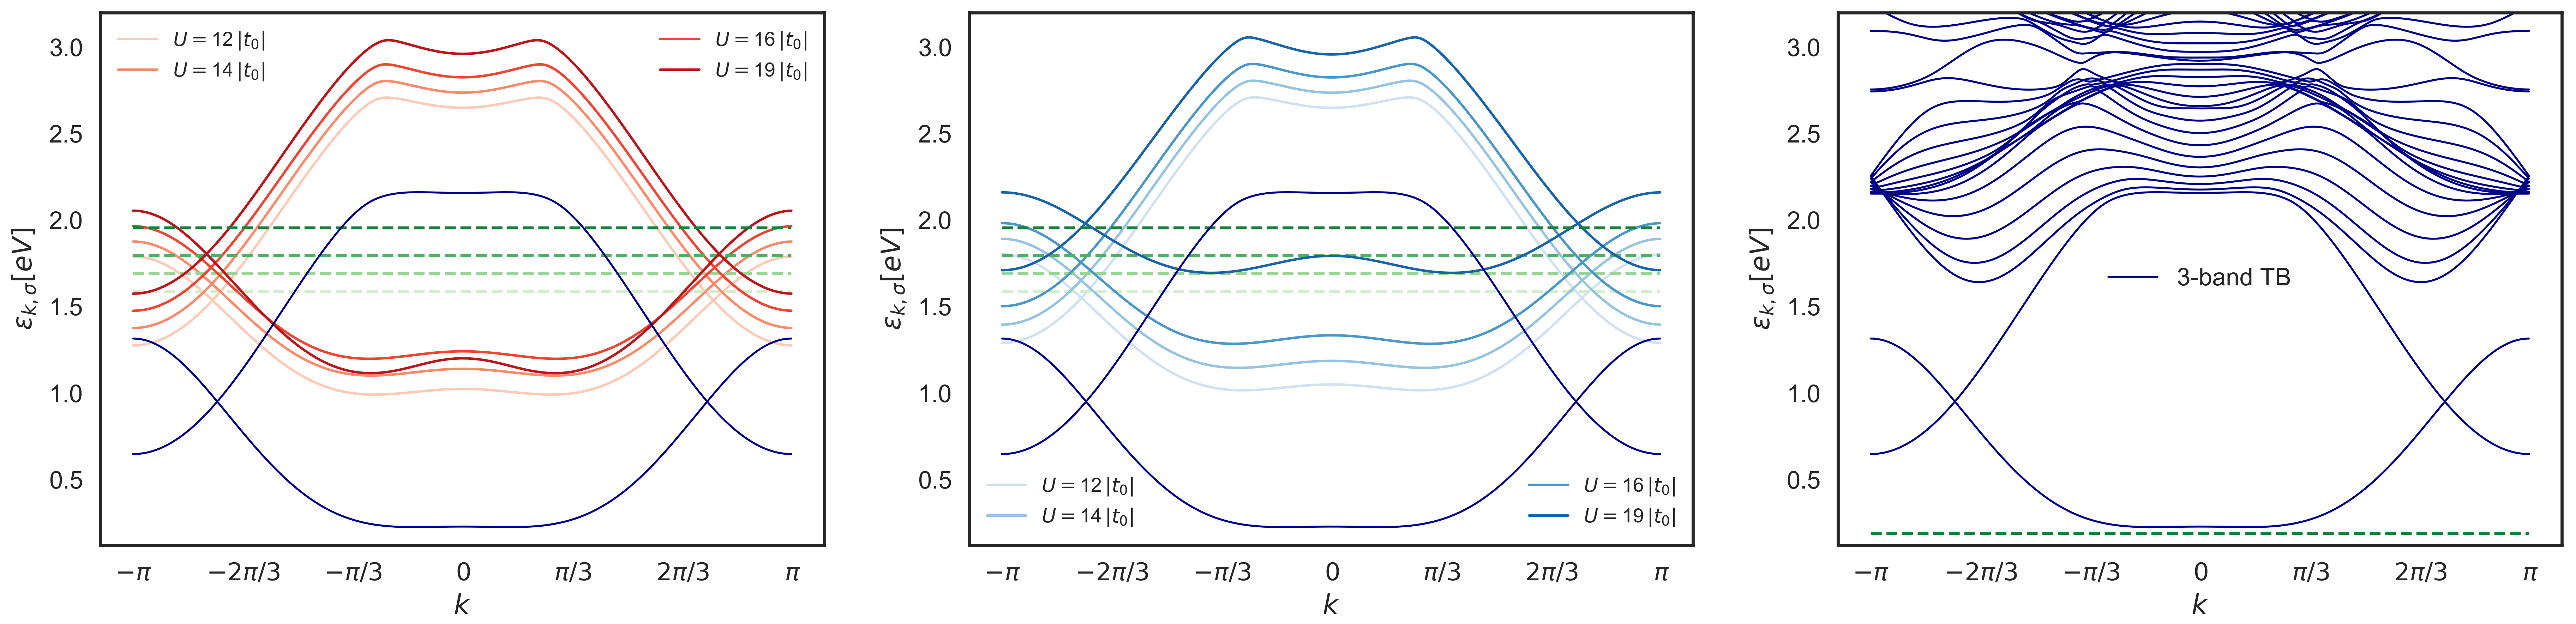
\includegraphics[scale=0.42]{Applications/tmd-mf/superposedBands05} \\
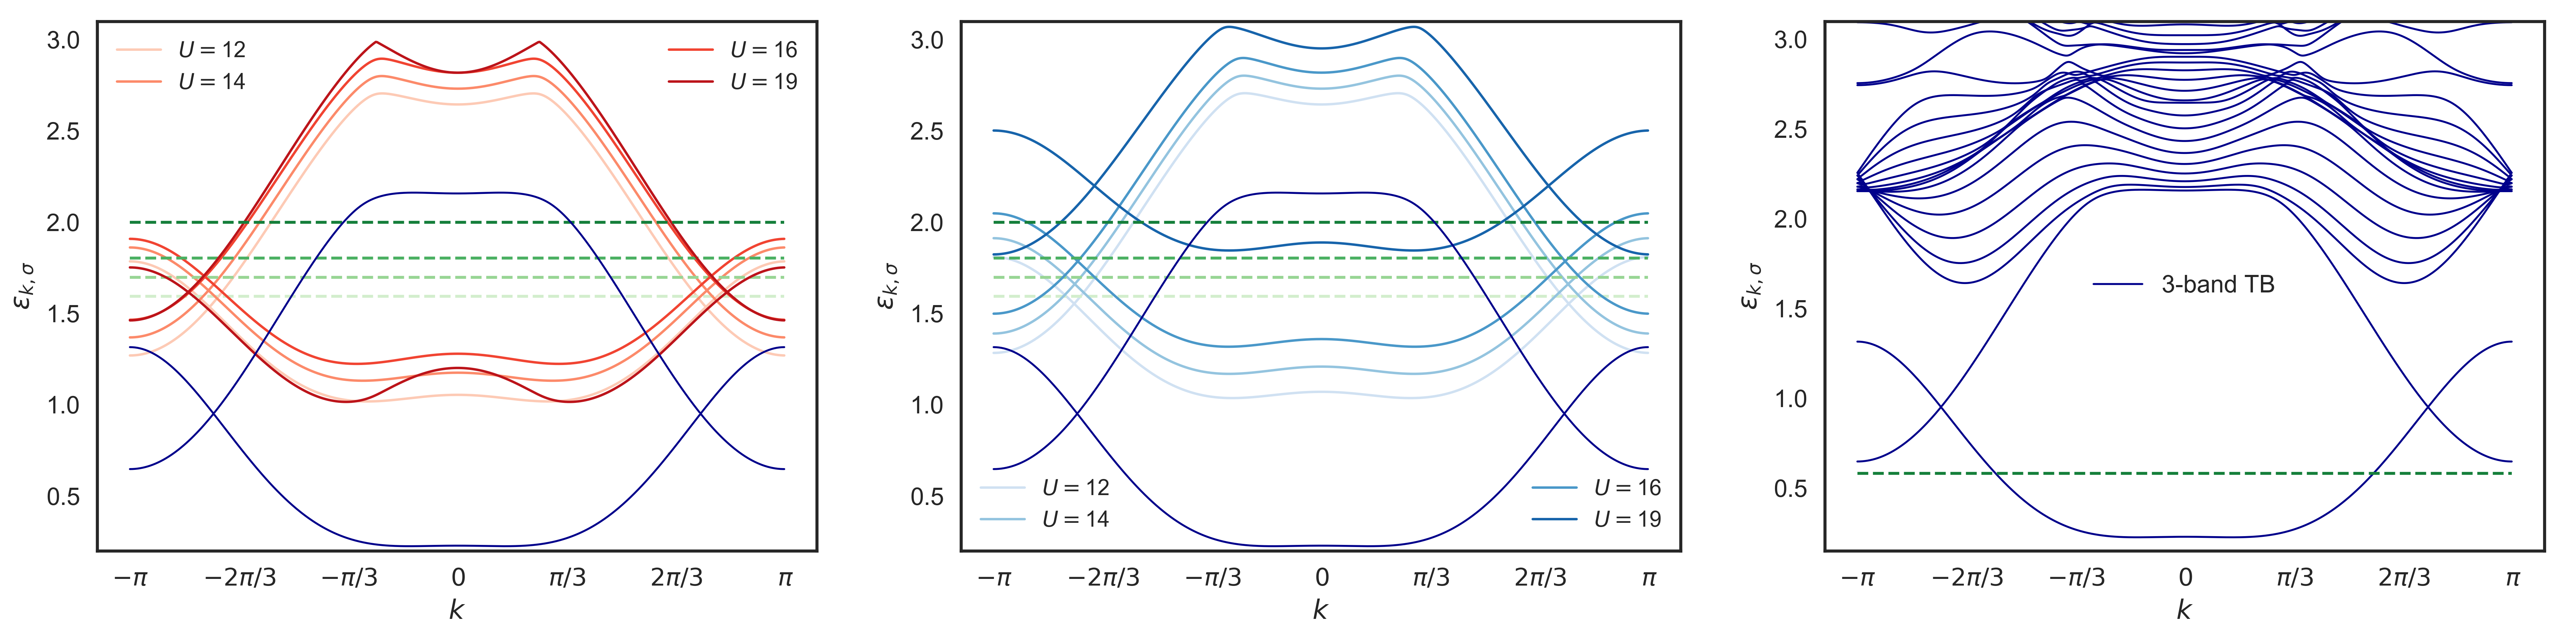
\includegraphics[scale=0.42]{Applications/tmd-mf/superposedBands075} \\
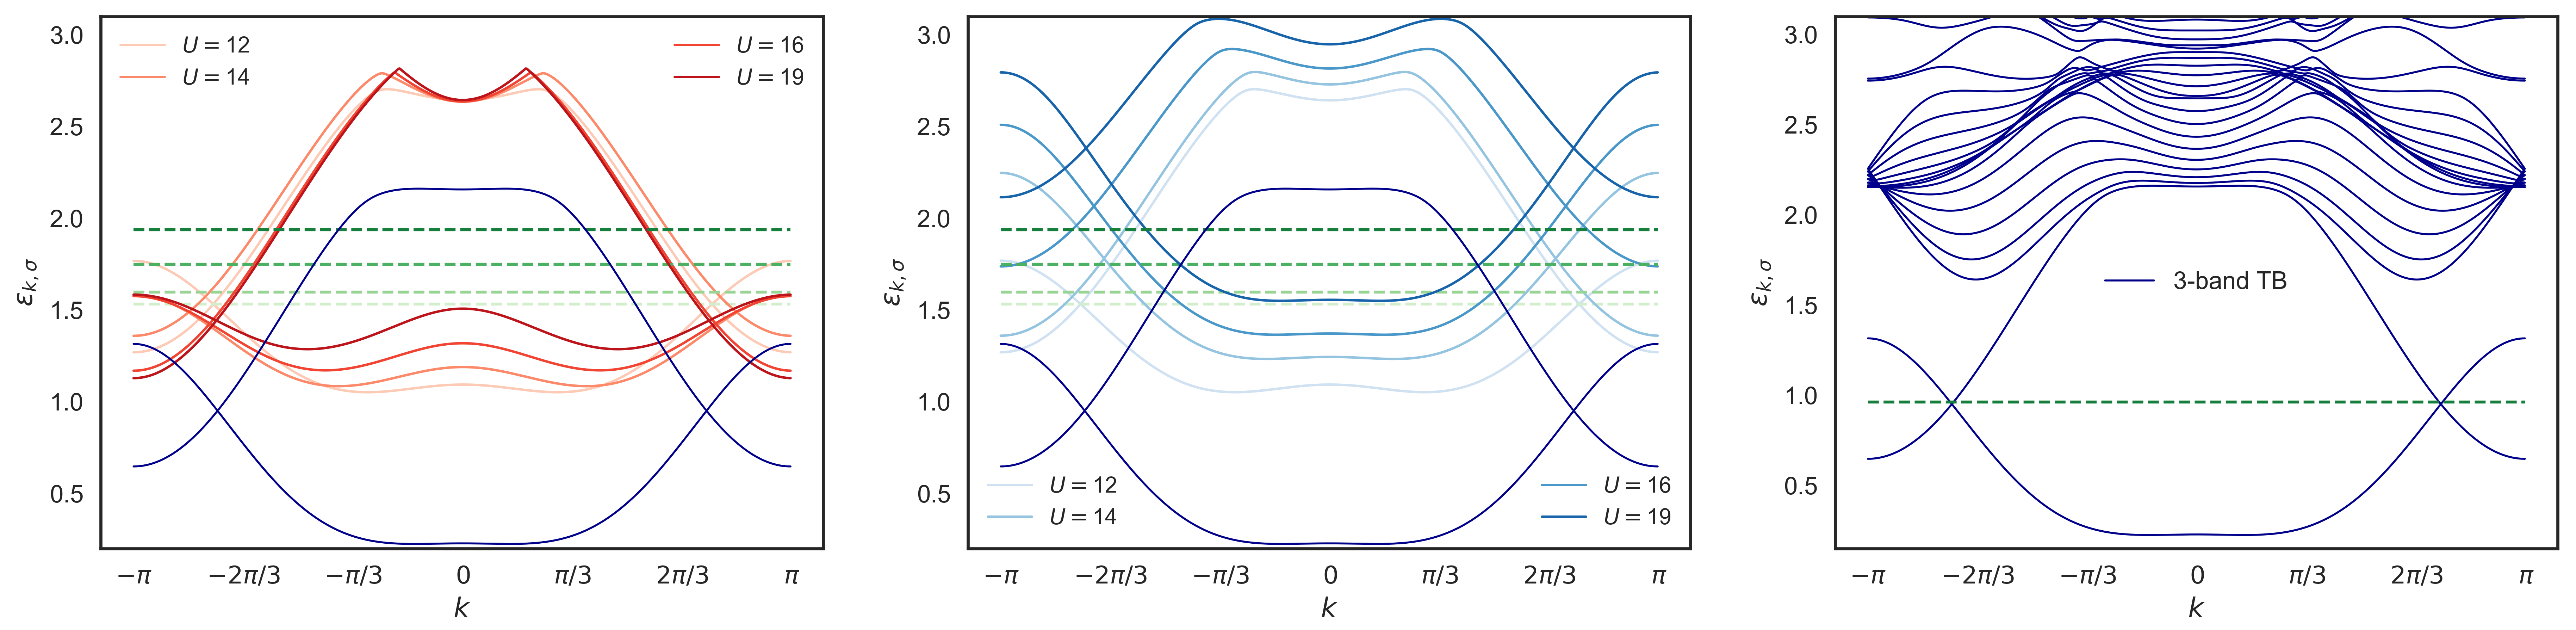
\includegraphics[scale=0.42]{Applications/tmd-mf/superposedBands4} \\
	\caption[Spin-resolved band structures for varying $U$ and $\beta$, compared with the tight-binding bands.]{Spin-resolved band structures for varying $U$ and $\beta$, compared with the tight-binding bands, demonstrating the changes in shape of the bands, and the change of the Fermi energy.
	From top to bottom, we have $\beta = (0.5, 0.75, 4)| t_0 |$.
	We can see that increasing $U$ leads to an increase in the Fermi energy, to compensate for the states that gain more energy, and that must be occupied to ensure charge neutrality.
	On the rightmost figures, we represent the Fermi energy that would correspond to the  considered temperature in the tight-binding case.}
	\label{fig:band-structures}
\end{figure}
The edge magnetization is due to the different occupation of the spin-up (in red) and spin-down bands (in blue).
As the red, spin-up band near the Fermi energy rests completely below it, its electronic states are all occupied, while the corresponding spin-down states are all above $\varepsilon_F$, and thus are unoccupied.
If these states were extended throughout the sample, a magnetization would appear in the bulk as well.
However, as we show later, the wave functions corresponding to the states near the Fermi energy are heavily localized at the edges.
This means that the spin polarization will be restricted to the edges.
Initially, the up and down states are equally occupied.
As we start increasing $U$, one of the bands (say, the up band) becomes more occupied than the other.
The states in this band correspond only to one of the edges.
Suppose it is the top edge.
As we keep increasing $U$, the band structure changes and eventually, the up band corresponding to the bottom edge becomes occupied than the down spin, bottom edge band, and both edges become magnetized.
In what follows, we explain how the two phase transitions we find can be understood in terms of the mean field picture we built.

In Fig.(\ref{fig:wfs1}), we can see that edge-magnetization has appeared on both sides of the ribbon.
An important detail to notice is that when the magnetization of the bottom edge appears at $U_{c_2} \approx 15.395 |t_0|$, the magnetization of the top edge decreases slightly.
This can be understood by looking at Fig.(\ref{fig:bandDegen}).
The band marked "$4$" has now \say{widened} (one can see that there is white space below it), and more down spin states localized at the top edge become occupied, canceling out some of the magnetization induced by their corresponding up spin states.
This effect occurs because, along with the lifting of the degeneracy, the Fermi energy increases slightly.
Finally, in Fig.(\ref{fig:pdMF}), we present a complete phase diagram, containing the behavior of the total edge magnetization $\left\langle m \right\rangle_{\text{edges}} = \left\langle m \right\rangle_{\text{top}} + \left\langle m \right\rangle_{\text{bottom}}$ for varying $U$ at a number of different inverse temperatures $\beta$ (here, $\beta$ is in units of $| t_0 |$).
\begin{figure}[H]
\hspace{0.8cm}
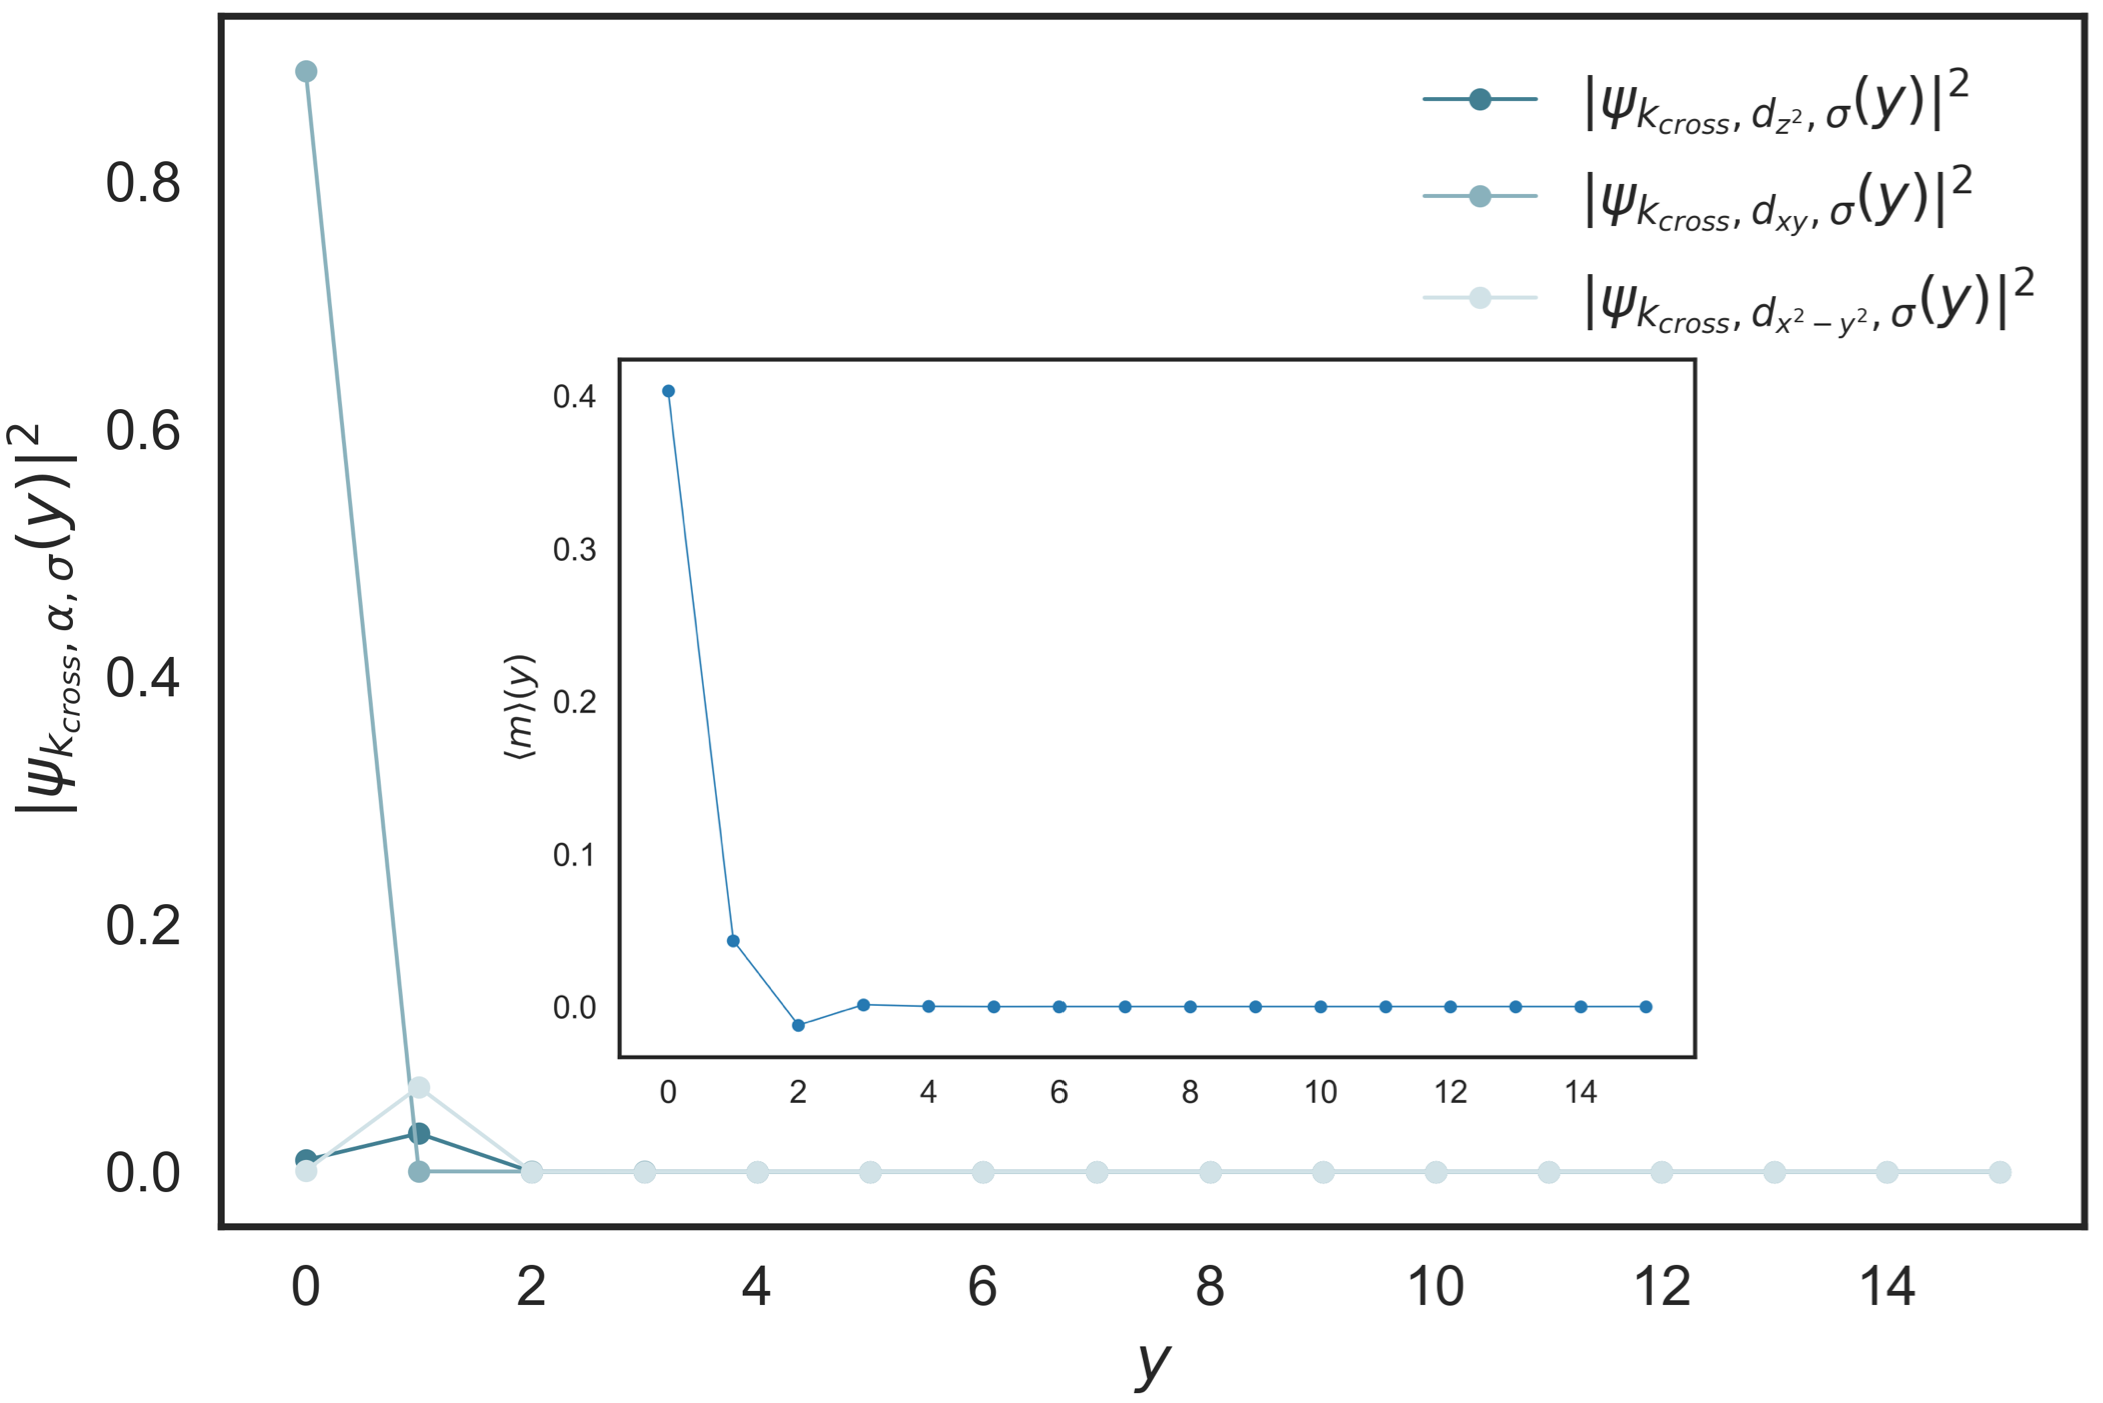
\includegraphics[scale=0.18]{Applications/tmd-mf/topEdgeMagProfU13}
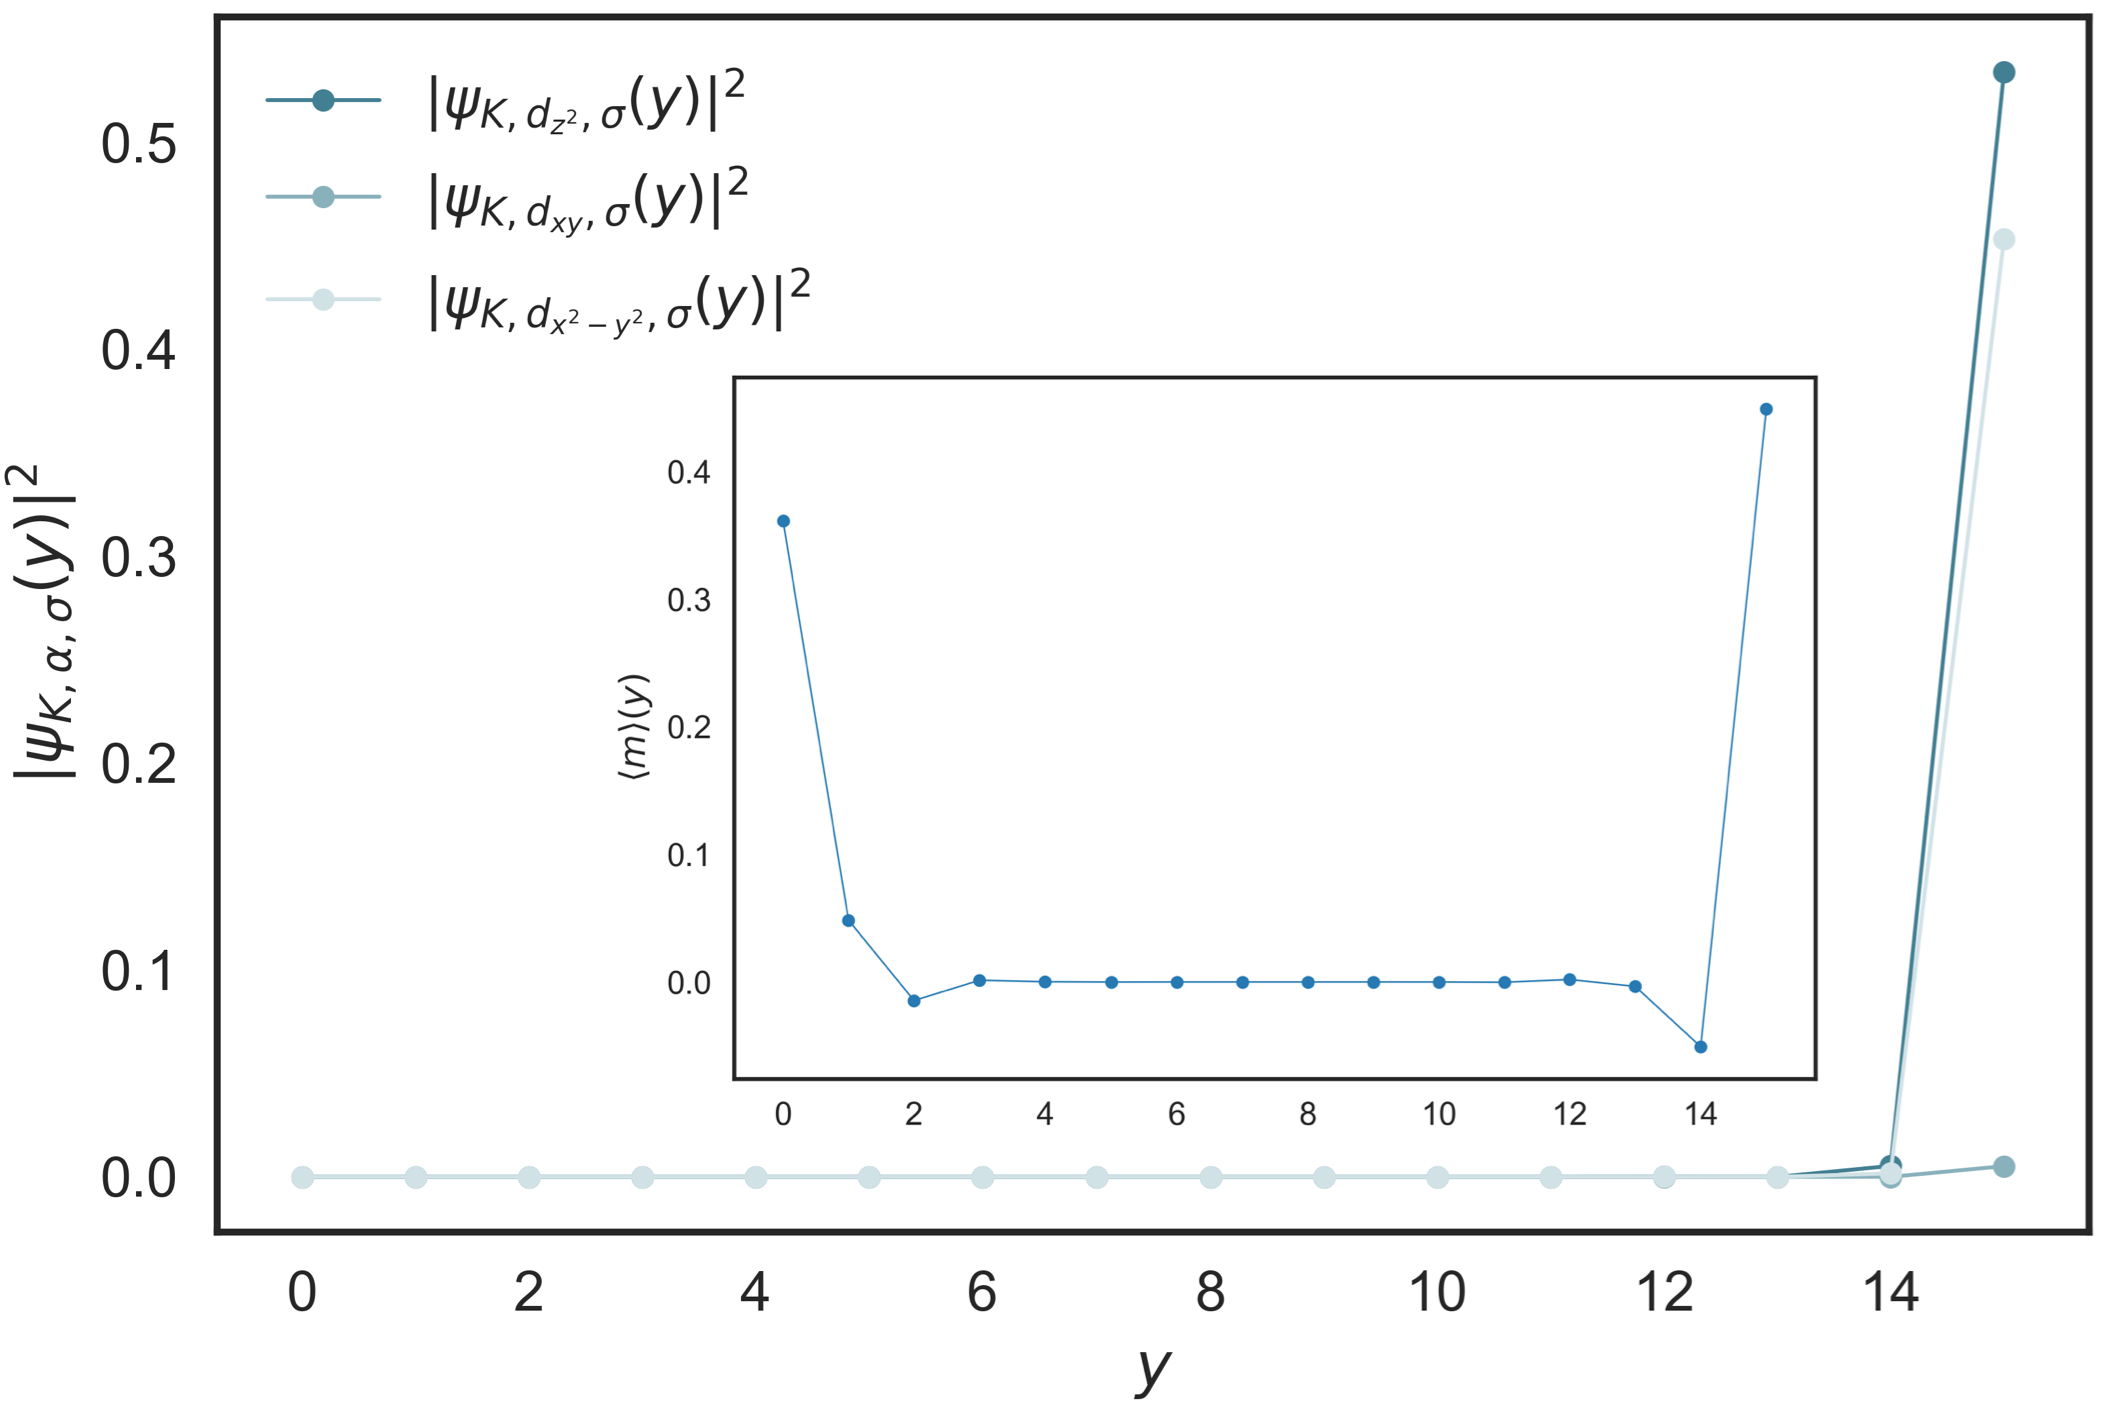
\includegraphics[scale=0.18]{Applications/tmd-mf/bottomEdgeMagProfU154}
	\caption[Localized edge states on the top and on the bottom of the ribbon for the different orbitals. Resulting magnetization profile along the ribbon's transverse direction due to higher spin up than spin down occupation.]{Left: Localized edge states on the top of the ribbon, at $U = 13 |t_0|$ (left) and on the bottom, at $U = 15.4 |t_0|$ (right) for the different orbitals. Insets: Resulting magnetization profiles along the ribbon's transverse direction due to higher spin up than spin down occupation of these states, showing, respectively top, and top-bottom edge magnetization.}
	\label{fig:wfs1}
\end{figure}
\vspace{-0.5cm}
\begin{figure}[H]
\hspace{0.3cm}
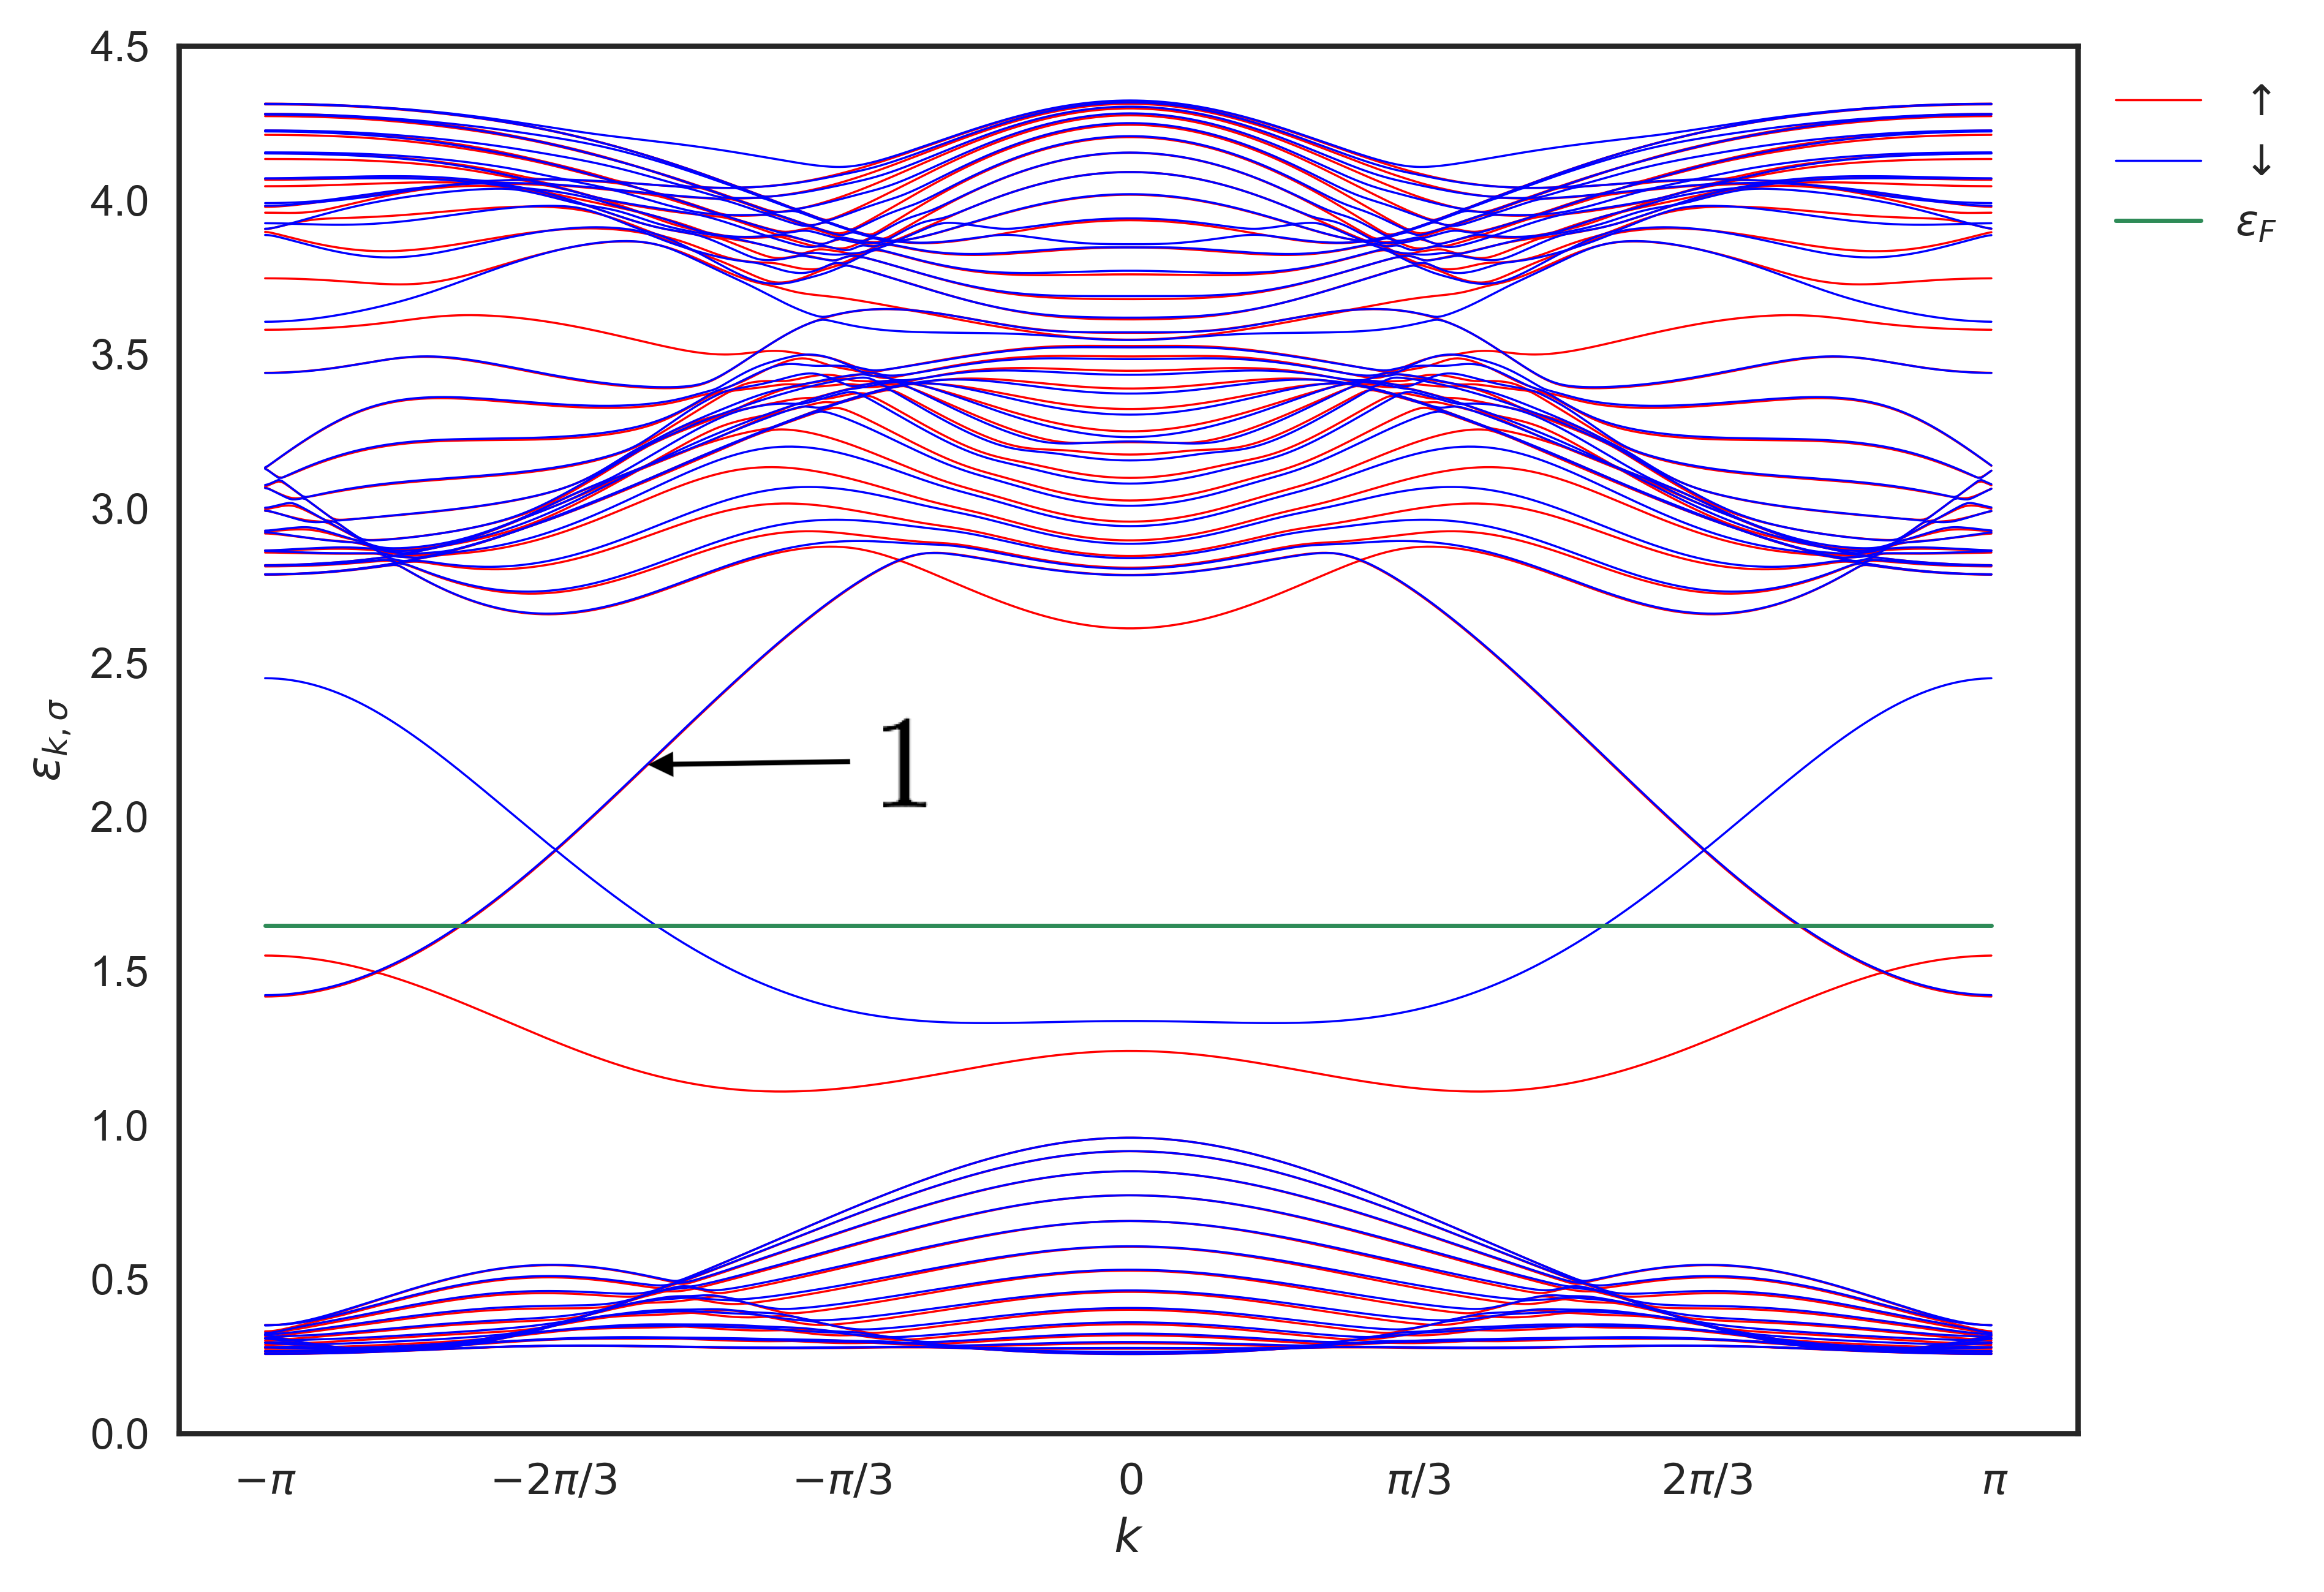
\includegraphics[scale=0.38]{Applications/tmd-mf/bands152.png}
\hspace{8mm}
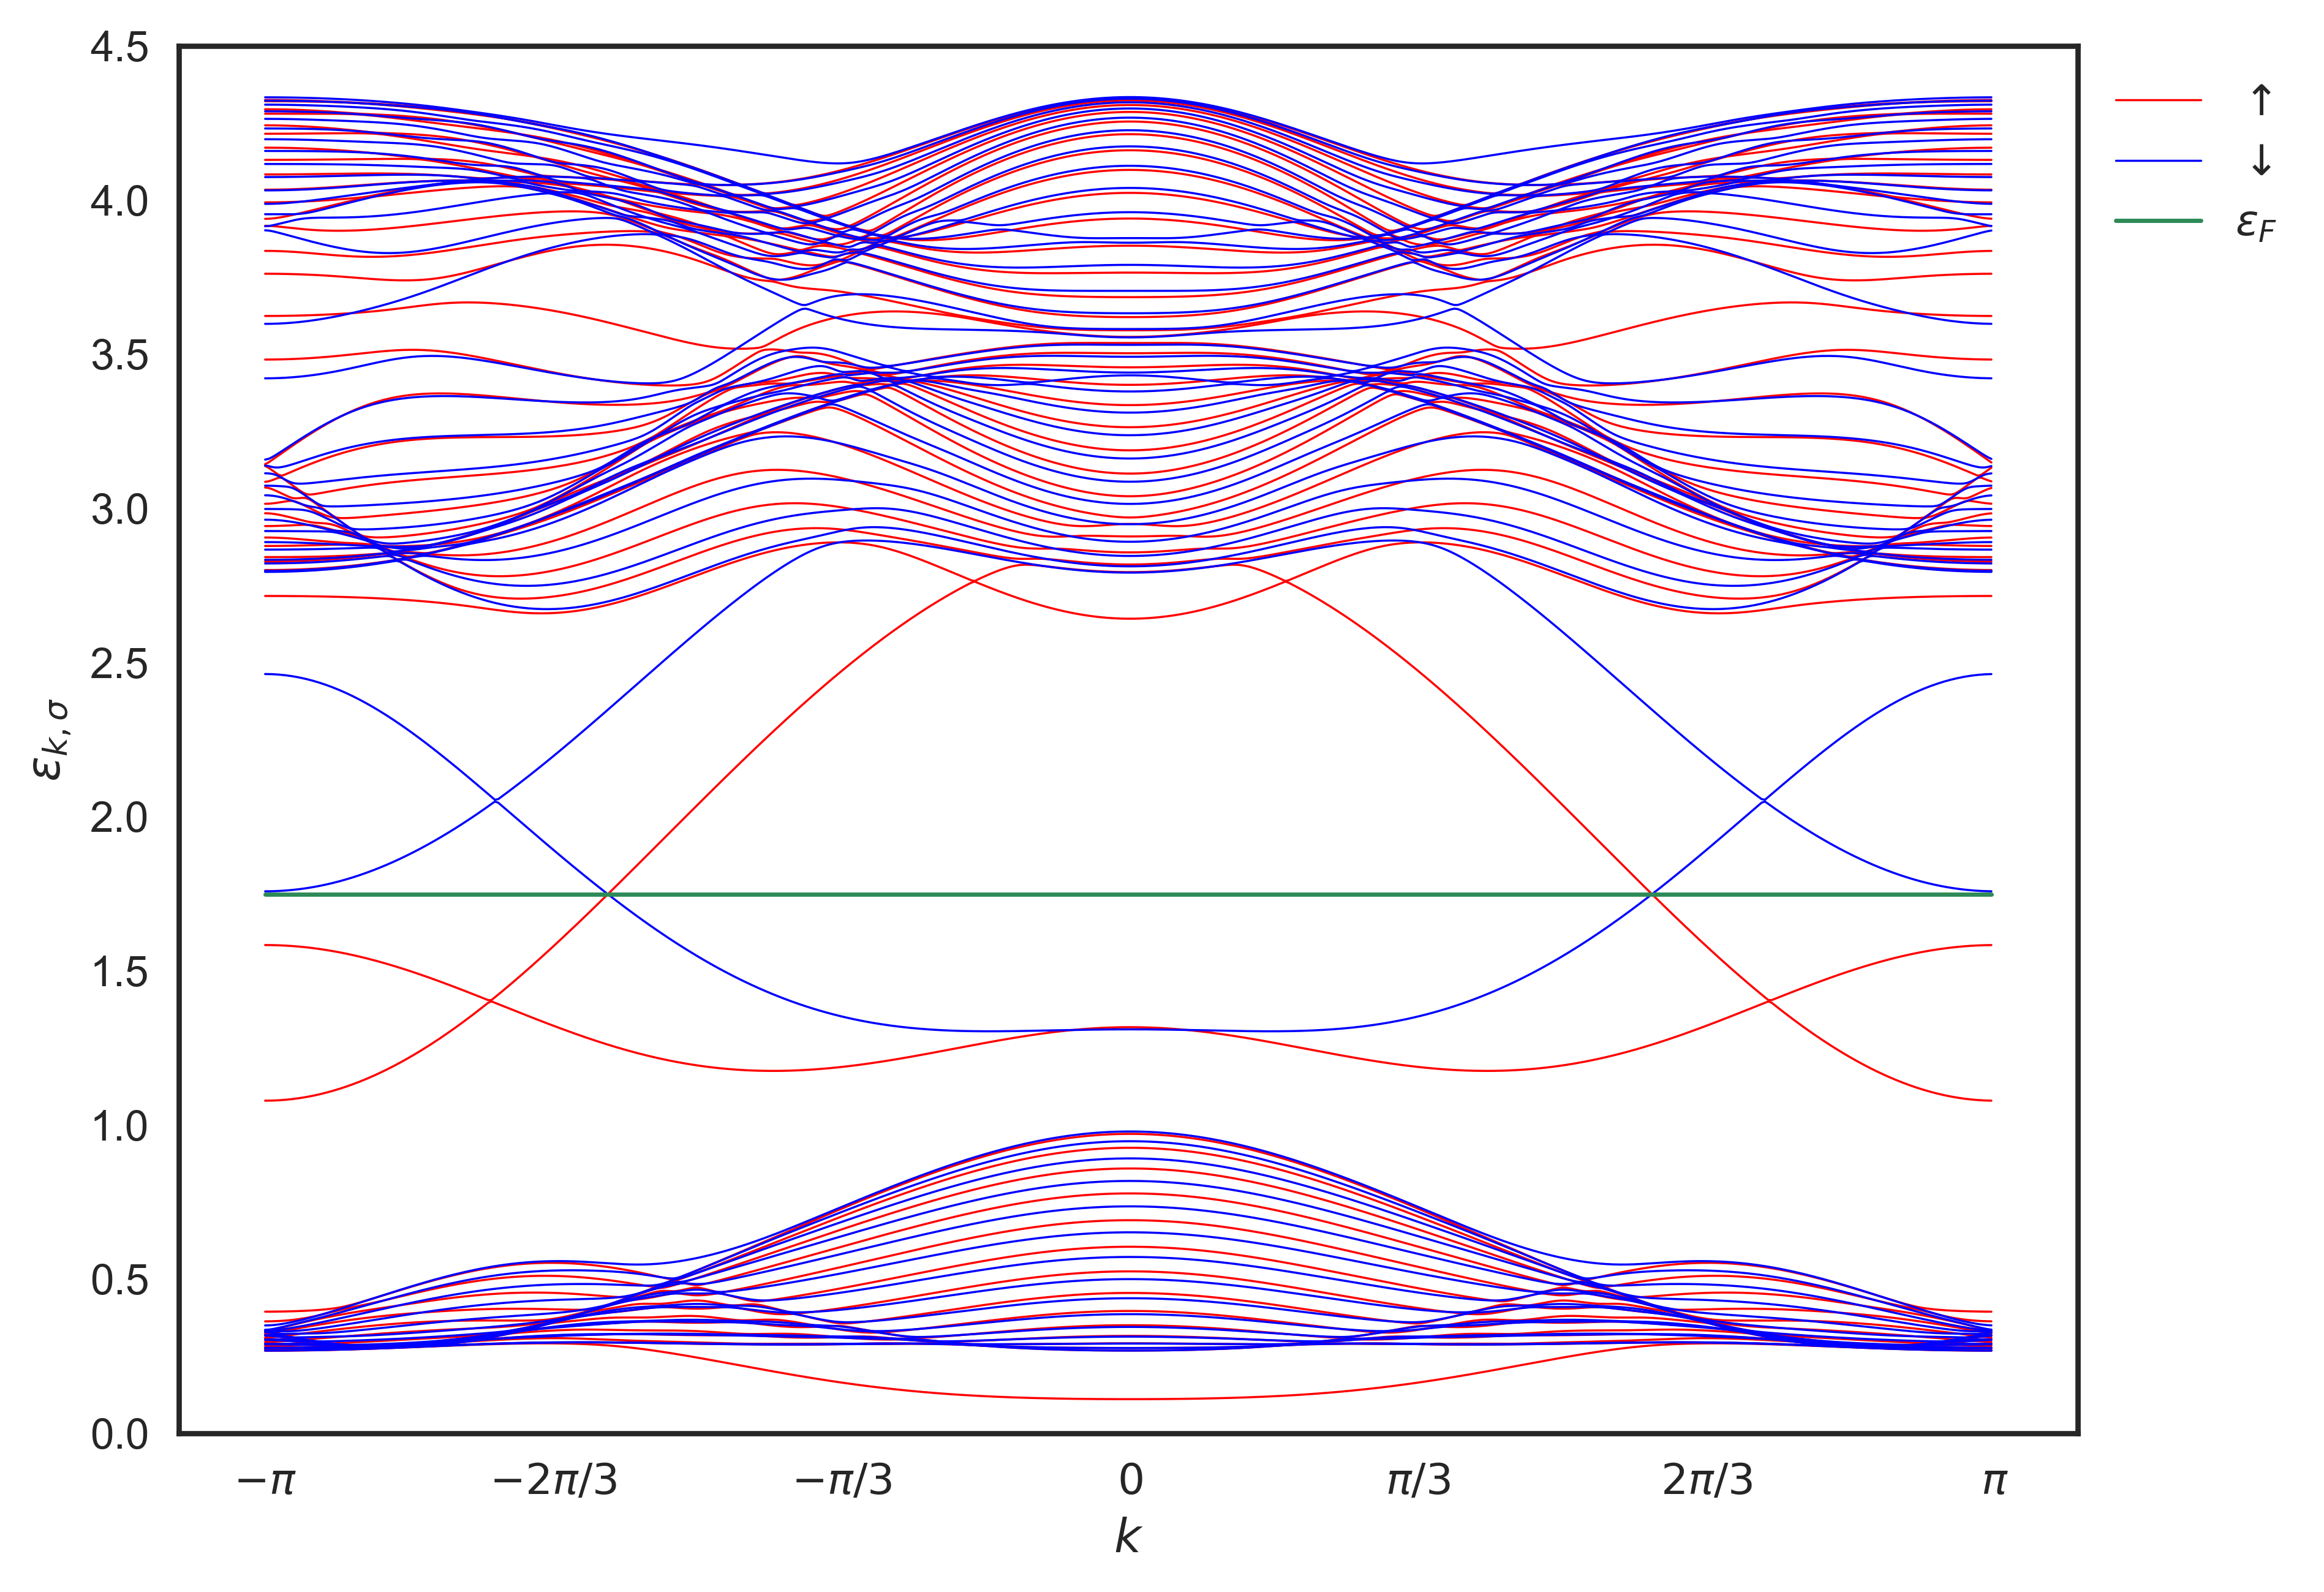
\includegraphics[scale=0.38]{Applications/tmd-mf/bands154.png}
	\caption[Comparison of the band structures at $U = 15.2| t_0 |$, and $U=15.4| t_0 |$.]{Comparison of the band structures at $U = 15.2| t_0 |$ (left), and $U=15.4| t_0 |$ (right). The second phase transition occurs because the degeneracy of the bands marked as "$1$" below $U = 15.395 | t_0 |$ is lifted, leading to the appearance of two bands, marked "$2$", and "$3$". Band 2 stays above the Fermi energy. Thus, it is unoccupied. Part of band 3 becomes occupied, leading to the magnetization of the edge (the states that become occupied are localized at the bottom edge).}
	\label{fig:bandDegen}
\end{figure}
\vspace{-0.6cm}
\begin{figure}[H]
\hspace{0.3cm}
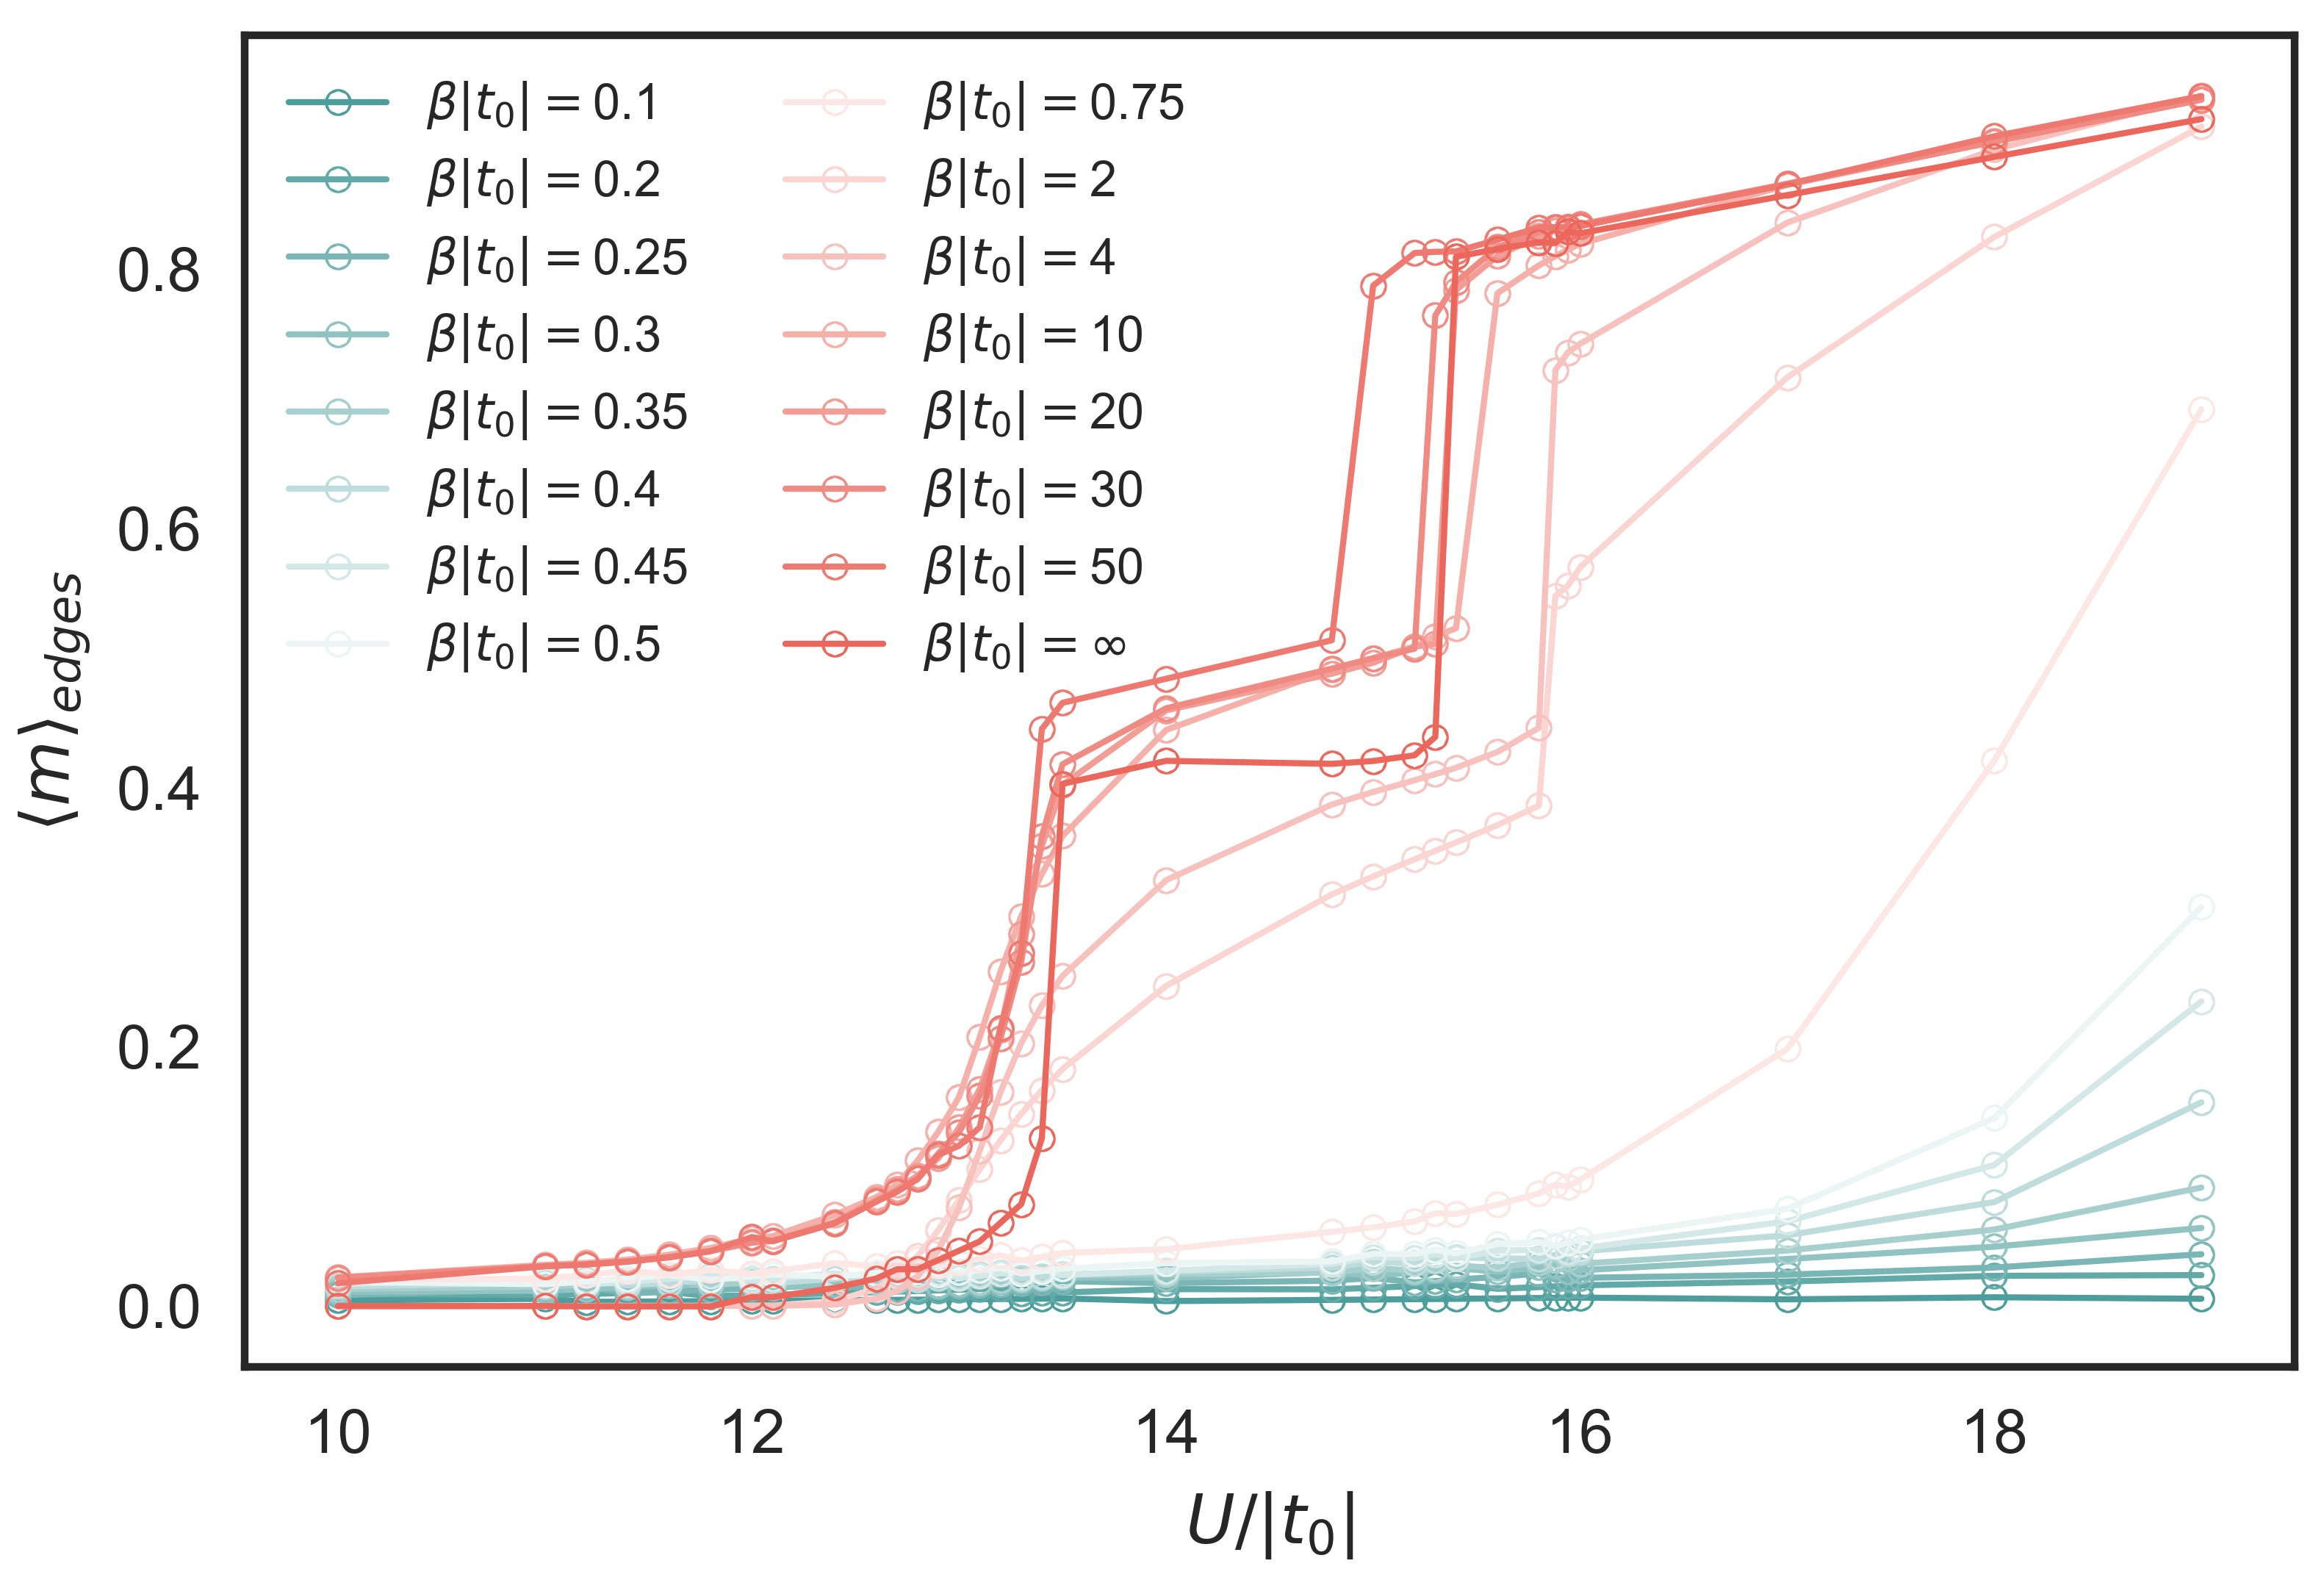
\includegraphics[scale=0.55]{Applications/tmd-mf/edge-mag-phase-diagram}
	\caption[Mean field phase diagram for varying $U$ and $\beta$. Average sign as a function of electron density, obtained by running our determinant \ac{QMC} code for a $9 \times 4$ \acs{TMDNR} at $\beta = 2| t_0 |$, $U = 16| t_0 |$.]{Left: Mean field phase diagram for varying $U$ and $\beta$. Right: Average sign as a function of electron density, obtained by running our determinant \ac{QMC} code for a $9 \times 4$ \acs{TMDNR} at $\beta = 2| t_0 |$, $U = 16| t_0 |$.}
	\label{fig:pdMF}
\end{figure}
\vspace{-0.3cm}
The first phase transition is suppressed at inverse temperature $\beta \lesssim 1 | t_0 |$, and for yet higher temperatures the second transition too is suppressed.
The critical on-site interactions $U_{c_{1, 2}}$ vary with temperature.
As $\beta$ is decreased from $\infty$ to $\beta \sim 10 | t_0 |$, the first transition occurs sooner, at about $U = 10 | t_0 |$, and the center plateau between the two transitions becomes shorter.
By $\beta = 2 | t_0 |$, the plateau has disappeared, $U_{c_1}$ returns to about its original ($\beta = \infty$) value, and the magnetization increases smoothly until $U_{c_2}$ (which is now higher than the original one at $\beta = \infty$ ).
Below $\beta = 0.75 | t_0 |$, the system smoothly increases its edge magnetization starting at $U \sim 12 | t_0 |$, and at about $\beta = 0.1 | t_0 |$, both transitions seem to be completely suppressed (in this range of $U$).

In Fig.(\ref{fig:pdMF}, right), we show an example of a result of our \ac{QMC} code for a \acs{TMDNR}.
On the lattice models considered so far, we took half filling, where (in the cases we had been discussing so far - bipartite lattices and particularly symmetric Hamiltonians) there is no sign problem (see appendix \ref{ap:theoAFQMC}).
In the model we consider, the sign problem severely restricts the range of parameters $U$, $\beta$, $\mu$ (or $\left\langle n \right\rangle$) that we can explore.
In fact, for $\beta > 2 | t_0 |$, the average sign rapidly goes to zero for the range of on-site interactions where mean field predicts the existence of an ordered phase.
Nonetheless, Fig.(\ref{fig:pdMF}, right) gives us a particularly good combination of parameters for which mean field predicts an ordered phase, and at the relevant electron density $\left\langle n \right\rangle = 0.66$, the sign problem is not prohibitive ($\left\langle \text{sign} \right\rangle \sim0.4$), so that our simulations can be used to extract information about the system.
However, the preliminar results of Fig.(\ref{fig:tmd-data}) indicate that the complexity of the problem is much higher than, for example, in the case of graphene.
Furthermore, recent analogous studies for graphene \cite{feldner_dynamical_2011, yang_strain-tuning_2017,raczkowski_interplay_2017} suggest that one needs thicker ribbons to measure long range ordering with enough accuracy, which implies taking larger system sizes.
To be conclusive about the true nature of edge-magnetism in \ac{TMDNR}s, given the increased complexity of our model, this requires an enormous amount of computer time (about 20 times, or possibly more than for the analogous graphene studies), which we shall have access to very soon.
\vspace{-0.25cm}
\begin{figure}[H]
\centering
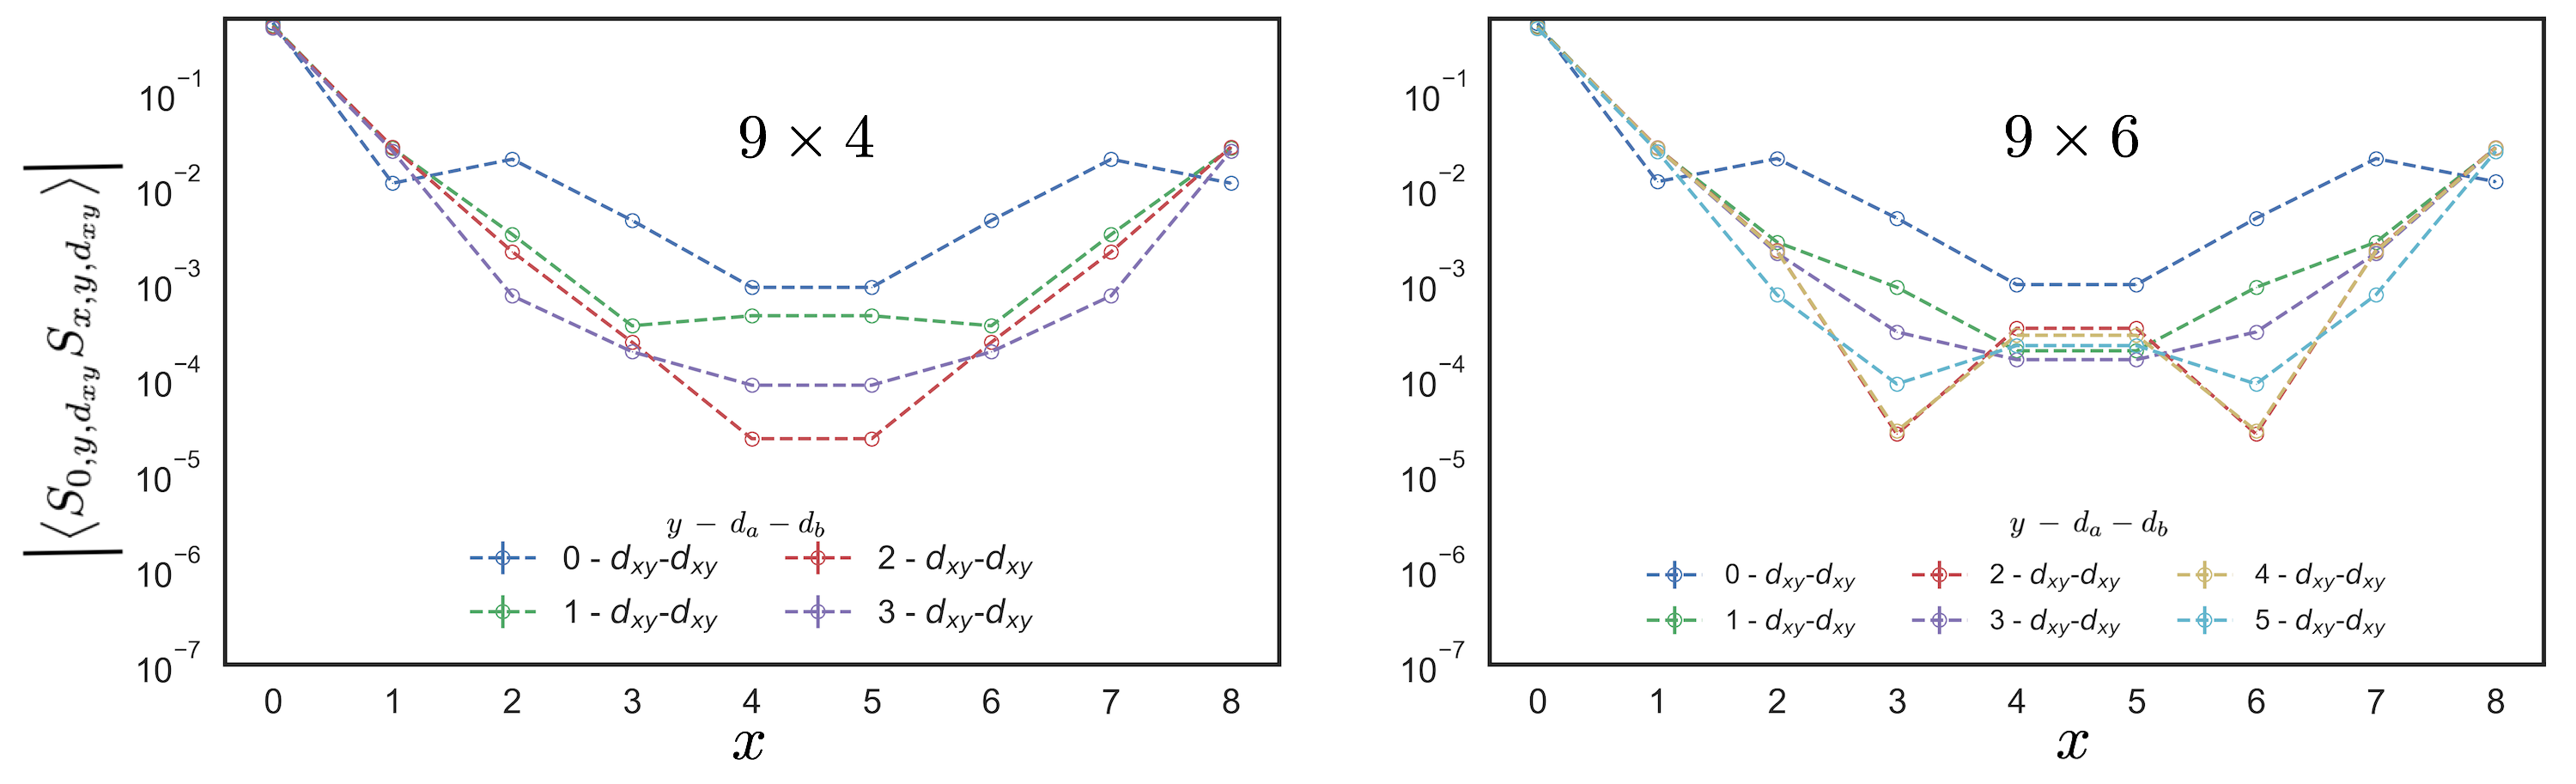
\includegraphics[scale = 1.07]{Applications/tmdFinalxyxy.png} \\
\hspace{-0.5cm}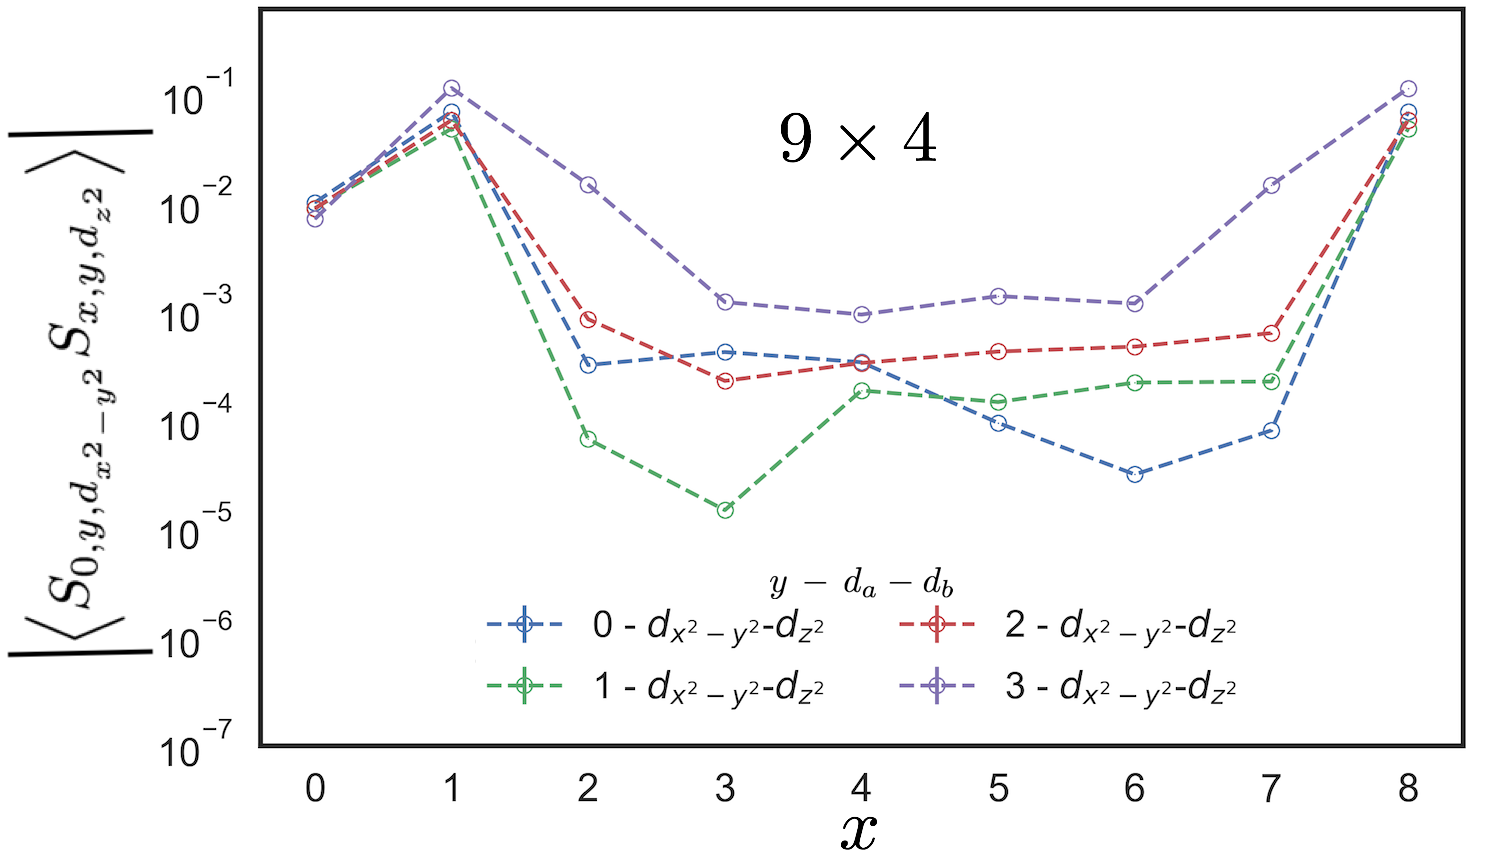
\includegraphics[scale = 1.08]{Applications/tmdFinalx2y2z2.png}
	\caption[Longitudinal profile (along the $x$ direction) of orbital-resolved $S^z$ spin-spin correlation functions we measured, for two lattice sizes: $9 \times 4$ and $9 \times 6$.]{Longitudinal profile (along the $x$ direction) of some of the orbital-resolved $S^z$ spin-spin correlation functions for two lattice sizes $9 \times 4$ and $9 \times 6$ ($d_{x^2-y^2} d_{z^2}$ and $d_{xy} - d_{xy}$).
	We use translational invariance along the $x$ direction to average these correlations to improve the statistical properties of the estimator.
	On the left, curves 0, and 3 show correlations along the edge rows, while on the right, curves 0 and 5 correspond to the edges.}
	\label{fig:tmd-data}
\end{figure}

